% =========================================================================
% CivicWorkOS -- Frontiers in Artificial Intelligence
% Article type: HYPOTHESIS AND THEORY
%
% The evaluation protocol this article specifies has NOT been executed. The
% evidentiary load is carried by Section 6 (the worked bridge-inspection
% allocation, its sensitivity frontier and two parameter shocks) and by the
% closed-form debt model of Section 9.1. Every number either article prints
% is exact arithmetic on stated inputs, a value of eq:cadmodel, or an
% explicitly labelled unexecuted target. Before adding a quantity here, add
% it to audit_numbers.py and confirm the gate passes; see
% REVISION-PROGRAMME.md.
% =========================================================================
\documentclass[utf8]{FrontiersinHarvard}

% ---------------------------------
% FRONTIERS-SAFE PACKAGES
% ---------------------------------

\usepackage[hyphens]{url}

\usepackage[nopatch=footnote]{microtype}

\usepackage{lineno}

\usepackage[singlespacing]{setspace}

\usepackage{subcaption}
\usepackage{array}
\usepackage{tabularx}
\usepackage{booktabs}
\usepackage{siunitx}
\sisetup{detect-all}
\usepackage{float}
\usepackage[dvipsnames]{xcolor}

\usepackage{tikz}
\usetikzlibrary{arrows.meta,positioning}

\usepackage{pgfplots}
\pgfplotsset{compat=1.18}

\usepackage{threeparttable}
\usepackage{multirow}
%\usepackage{enumitem}
\usepackage{etoolbox}

\usepackage{pifont}
\usepackage{placeins}
\usepackage{algorithm}
\usepackage{algorithmicx}
\usepackage{algpseudocode}
\usepackage{xr}
\externaldocument{CivicWorkOS_supplementary}

\definecolor{civicgray}{RGB}{88,96,105}
\definecolor{civicblue}{RGB}{45,91,150}
\definecolor{civicteal}{RGB}{38,132,130}
\definecolor{civicamber}{RGB}{220,150,45}

\newcolumntype{Y}{>{\centering\arraybackslash}X}
\newcolumntype{C}[1]{>{\centering\arraybackslash}p{#1}}

\newtheorem{Proposition}{Proposition}

\providecommand{\descriptionlabel}[1]{\hspace\labelsep\normalfont\bfseries #1}
\newenvironment{description}
  {\list{}{\labelwidth=0pt \itemindent=-\leftmargin \let\makelabel\descriptionlabel}}
  {\endlist}

\AtBeginEnvironment{tikzpicture}{\nolinenumbers}
\AtEndEnvironment{tikzpicture}{\linenumbers}

\linenumbers

% ---------------------------------
% FRONTIERS META
% ---------------------------------
\def\firstAuthorLast{Syed et~al.} % for running header


\def\Authors{
	Toqeer Ali Syed$^{1}$,
	Ali Akarma$^{1,2}$,
	Raghda M. Alqurashi$^{3,*}$,
	Muhammad Tayyab Naqash$^{4}$,
	Abdulaziz Alqurashi$^{4}$
}

\def\Address{
	$^{1}$AI Center, Faculty of Computer and Information Systems, Islamic University of Madinah, Madinah, Saudi Arabia\\
	$^{2}$AI V\&V Lab, King Fahd University of Petroleum and Minerals, Dhahran, Saudi Arabia\\
	$^{3}$Department of Computer Science, Umm Al-Qura University, Jumum, Saudi Arabia\\
	$^{4}$Civil Engineering Department, Islamic University of Madinah, Madinah, Saudi Arabia
}

\def\corrAuthor{Raghda M. Alqurashi}
\def\corrEmail{rmqurashi@uqu.edu.sa}



\begin{document}
	\onecolumn
	\firstpage{1}

	\title[CivicWorkOS]{CivicWorkOS: Capability-Preserving Allocation of Municipal Work Among Humans, AI Agents and Robots}

	\author[\firstAuthorLast]{\Authors}
	\address{}
	\correspondance{}
	\extraAuth{
		\textbf{Article type:} Hypothesis and Theory \\
		\textbf{Word count:} approx.\ 18,500 \\
		\textbf{Number of figures:} 3 \\
		\textbf{Number of tables:} 13
	}

	\maketitle
	\footnotetext{$\dagger$ These authors contributed equally to this work and share first authorship.}


	\begin{abstract}
		Cities are moving from sensing infrastructure to agentic operation, in which AI agents perform administrative work and robots perform physical work. Allocation research optimizes fit, throughput, and ergonomics; labor research examines displacement; neither prices the developmental practice through which cities form their future practitioners. We present CivicWorkOS, which makes municipal allocation a governed decision over \textit{staffed modes} --- pairings of an execution mode with a named roster at declared career stages --- rather than a human-versus-machine choice. Civic Automation Debt prices five deferred liabilities, and four constraints bind the objective: a Human Capability Preservation Budget denominated in qualified-practice hours accruing only to practitioners below independent competence, a Capability Access Constraint governing who receives protected practice, a Just Transition Constraint, and an N$-$1/N$-$2 resilience reserve. We give the city-wide program, an online Lagrangian rule with bounded between-rebalance violation, a feasibility condition, and an intake requirement for when the budget is unattainable. An exact bridge-inspection instance, reproducible by direct arithmetic from the reported values, prices protected practice at 0.0454 objective units per hour, costs 4.34\% of annual objective value (0.33--9.60\% across the swept parameter frontier), and yields 3.46 competent-equivalents a year against attrition of 2.88. The same arithmetic produces a result no headcount plan surfaces: machine-assisted supervised practice stretches time to competence by a factor of 3.38, from 1.2 to 4.05 years, so a city sizing intake from certification hours provisions four trainee posts where fourteen are required.
	\end{abstract}


	\section{Introduction}
	\label{sec:intro}
	
	Urban automation has changed character. Traditional smart-city systems sensed, connected, and analyzed urban data. Agentic systems additionally plan, decide, negotiate, invoke tools, and act, while autonomous robots physically execute those decisions in public space. Choi and Yoon~\cite{Choi2025} demonstrate AI-agent-based urban digital twins operating over live municipal data, and Shariatpour et al.~\cite{Shariatpour2026} describe the resulting shift toward ``agentic cities'' in which urban infrastructures sense, learn, predict, and act.
	
	This creates a distributional question that no existing allocation mechanism answers. A bridge inspection may be performed by a licensed inspector, a computer-vision agent, an autonomous robot, or a mixed team. A citizen service request may be handled by a public employee, an AI agent, or a human supervised by one. Sanitation, maintenance, transport, logistics, emergency response, and administration decompose the same way. Every such decision has a winner and a loser, and cities currently make them without any mechanism that records who lost what.
	
	The policy problem is not whether AI and robots will replace municipal workers. It is how a city should continuously decide which tasks are automated, augmented, reserved for humans, or performed by hybrid teams, and, having decided, who performs the work that remains.
	
	We treat that second half as constitutive. Automation exposure is not distributed evenly across occupational class, gender, contract status, or district~\cite{AcemogluRestrepo2020,Eloundou2024}, and neither is the developmental work that turns a novice into an expert. A municipality that automates its junior inspection, triage, and casework tasks is not only reducing headcount. It is closing the route by which its next generation of senior practitioners would have been formed, closing it first for whoever was next in line, and doing so invisibly both to a productivity objective and to an equity audit conducted after deployment, because it operates one locally defensible task at a time.
	
	\subsection{Contributions}
	\label{sec:contributions}
	
	This article contributes the following.
	
	\begin{itemize}
		\item A city-scale allocation formalism whose decision variable is a \textit{staffed mode}, a pairing of an execution mode with a roster of named practitioners at declared career stages. This is what makes the distributional questions answerable: mode selection alone cannot express who receives the work.
		\item \textit{Civic Automation Debt}, pricing the deferred liability created by skill-formation loss, fallback erosion, accountability dilution, vendor dependency, and labor-transition burden. We claim no novelty for the underlying concern, which Bainbridge~\cite{Bainbridge1983} stated for the individual operator. The contribution is its aggregation to a municipal workforce, its formal separation from the immediate-outcome terms with which it is routinely confused, and its entry into a decision as a priced quantity with a computable flip threshold.
		\item A \textit{Human Capability Preservation Budget} in qualified-practice hours that accrues only to practitioners below independent competence, with a stated unit conversion from raw certification hours, an explicit feasibility condition, and a \textit{capability intake requirement} that tells a city how many developing practitioners the budget implies when the constraint cannot otherwise be met.
		\item A \textit{Capability Access Constraint} governing who receives protected practice, so a budget sized from the incumbent workforce does not reproduce its composition for a replacement cycle, together with the equality-law and data-protection analysis that a mechanism allocating work by protected characteristic requires.
		\item A \textit{Policy Digital Twin} with a defeasible rule language, a status lattice, a conflict-resolution order, and a worked encoding of an EU AI Act oversight obligation, plus \textit{Adaptive Oversight Zones} with specified transition predicates and a zone-to-mode mapping.
		\item The city-wide assignment program the coupled constraints require, an online Lagrangian approximation with duals for every coupling constraint and a bounded between-rebalance violation, and a bridge-inspection allocation carried through end to end: a six-way sensitivity sweep, a stated feasibility frontier, and two parameter shocks on either side of it, all by exact arithmetic on the reported values.
		\item An evaluation protocol for the framework, specified in full with ten hypotheses and explicit refutation criteria calibrated against that allocation. The protocol has not been executed, and no claim in this article rests on an outcome of it. We state it so the evaluation the framework requires is fixed in advance and auditable rather than reconstructed once results are in hand.
	\end{itemize}
	
	Section~\ref{sec:relatedwork} reviews related work and states the gap and research questions. Section~\ref{sec:framework} defines Civic Automation Debt and the framework's layers. Section~\ref{sec:architecture} gives the architecture, optimization program, algorithm, and formal results. Section~\ref{sec:governance} covers governance, contestability, lawfulness, and data protection. Section~\ref{sec:worked} works the bridge-inspection allocation end to end, with its sensitivity frontier and two parameter shocks. Section~\ref{sec:discussion} interprets what that establishes and what it does not, specifies the evaluation protocol the framework requires and has not undergone, and states the limitations. Section~\ref{sec:conclusion} concludes.
	
	\section{Related Work and Research Gap}
	\label{sec:relatedwork}
	
	\subsection{Human--Robot and Human--AI Task Allocation}
	\label{sec:rw-hrta}
	
	Ranz et al.~\cite{Ranz2017} proposed capability-based task allocation by matching task requirements to human and robot capabilities, establishing that allocation should depend on task--agent fit rather than on automation for its own sake, and Dorri et al.~\cite{Dorri2018} situate this within multi-agent systems theory, surveying the coordination and negotiation mechanisms that later allocation-market designs, including ours, build upon. Subsequent work expanded the criteria. El Makrini et al.~\cite{Makrini2019} considered ergonomics in collaborative assembly. Merlo et al.~\cite{Merlo2023} proposed dynamic role allocation using AND/OR graphs and ergonomic risk estimation, redirecting high-risk actions away from humans. Noormohammadi-Asl et al.~\cite{Noormohammadi2025} incorporated human leading and following preferences into adaptive robot planning, and Ali et al.~\cite{Ali2022} model artificial trust explicitly, re-optimizing allocation as measured trust evolves. Meseguer-Valenzuela and Blanes Noguera~\cite{MeseguerValenzuela2025} review allocation for mobile robot fleets, close to the sanitation, inspection, and logistics fleets a city must coordinate, and Hady et al.~\cite{Hady2025} survey multi-agent reinforcement learning for resource allocation. At city scale, Zhao et al.~\cite{Zhao2023} allocate spatio-temporal sensing tasks across a mobile crowd using a knowledge graph, which is the closest published treatment of municipal task allocation as a graph-structured assignment problem.
	
	These contributions target an operational team and optimize performance, productivity, ergonomics, preferences, or trust. They do not ask whether repeated local decisions erode the human experience needed to sustain future expertise, emergency substitution capacity, or resilience, nor, when that erosion occurs, whose expertise is eroded first.
	
	\subsection{Workforce Scheduling with Skill and Training Constraints}
	\label{sec:rw-sched}
	
	The operations-research literature has treated constrained training-hour allocation for fifty years, and the capability budget of Section~\ref{sec:hcpb} is a member of that family rather than a departure from it. Burke et al.~\cite{Burke2004} survey nurse rostering, where skill mix, supervision ratios, and qualification maintenance appear as hard constraints on a staffing decision, and Van den Bergh et al.~\cite{VandenBergh2013} review personnel scheduling more broadly, including the cross-training and skill-acquisition variants that decide how many staff reach a given competence by a given date.
	
	Two differences matter for a municipal allocation mechanism. Rostering assumes the work exists and asks who covers it. Our decision is prior: whether the work is performed by a human at all, and therefore whether the developmental content exists to be allocated. And rostering optimizes coverage subject to skill constraints, whereas the objective here prices the future value of the practice itself. What we take from this literature is its discipline about supervision ratios and qualification accounting, which is exactly what Section~\ref{sec:hcpb} repairs relative to earlier presentations of this framework.
	
	\subsection{Automation, Skill Erosion, and Capability Formation}
	\label{sec:rw-skill}
	
	The concern at the center of this paper is not new, and we want its lineage on the record before claiming anything. Bainbridge~\cite{Bainbridge1983} identified the ironies of automation: automating the easy parts of a task degrades operator skill through disuse and leaves the human unable to intervene competently at exactly the moment intervention is required. Endsley and Kiris~\cite{EndsleyKiris1995} formalized the resulting out-of-the-loop performance problem, and Parasuraman and Riley~\cite{ParasuramanRiley1997} organized the failure modes into use, misuse, disuse, and abuse. Sheridan and Verplank~\cite{SheridanVerplank1978} supplied the levels-of-automation scale, generalized by Parasuraman et al.~\cite{Parasuraman2000} across information acquisition, analysis, decision, and action. Shneiderman~\cite{Shneiderman2020} recasts the trade-off as two independent axes of automation and human control, and Zuboff~\cite{Zuboff1988} draws the organizational distinction between automating and informating work, which is the distinction between a task that displaces a practitioner and one that develops them.
	
	The quantitative basis for calibrating skill loss also exists. Arthur et al.~\cite{Arthur1998} meta-analyzed skill decay over non-use intervals across task types, and Tatel and Ackerman~\cite{TatelAckerman2025} update that estimate for procedural skills specifically, reporting retention as a function of retention interval, task closed-loop character, and rehearsal. These are the instruments a city would use to calibrate $D^{skill}$ against observed practice gaps rather than against expert judgment alone.
	
	Three consequences follow. The mechanism of skill erosion is established, so CivicWorkOS must not claim to have discovered it. That literature is written at the scale of the individual operator, whereas the municipal question, whether a city's whole expertise pipeline is drawn down across thousands of independent decisions in dozens of services, is what we address. And it warrants treating fallback capacity as distinct from present competence, which is why $D^{fall}$ is separated from $D^{skill}$ in Section~\ref{sec:problem}.
	
	The debt framing likewise has a source. Cunningham~\cite{Cunningham1992} introduced technical debt as the deferred cost of an expedient implementation choice, and Sculley et al.~\cite{Sculley2015} extended it to machine-learning systems, where the accumulating liability is configuration, data dependency, and entanglement rather than code. Civic Automation Debt is the same accounting move applied to a public workforce: a locally optimal allocation creates a liability settled later, by someone else, invisible on the ledger that authorized it. Rashidi~\cite{Rashidi2026} carries the concern into the agentic-AI era, arguing that AI is the first technology capable of automating the entry-level cognitive work through which expertise and professional judgment are formed.
	
	\subsection{Fair Division and the Distribution of Scarce Opportunities}
	\label{sec:rw-fair}
	
	Protected developmental practice is a scarce, valuable, and unequally distributed good, which places the Capability Access Constraint of Section~\ref{sec:access} inside the fair-division literature. Bouveret et al.~\cite{Bouveret2016} survey fair allocation of indivisible goods and the standard solution concepts, proportionality, envy-freeness, and their relaxations, and Caragiannis et al.~\cite{Caragiannis2019} show that maximizing Nash social welfare achieves envy-freeness up to one good together with Pareto optimality.
	
	We use a share constraint against a policy-set target rather than an envy-based criterion, and the reason is institutional rather than technical. Envy-freeness is defined over agents' own valuations of the bundles they receive, whereas a municipal panel must defend a distribution against a statutory equality duty and a published labor-pool composition, which are external standards. A Nash-welfare objective over practitioner valuations would also make the allocation depend on elicited worker preferences that no city currently records and that would be strategically reported if it did. The cost of this choice is that our constraint offers no envy guarantee, which we state plainly in Section~\ref{sec:limitations}.
	
	\subsection{Contestability and Algorithmic Due Process}
	\label{sec:rw-contest}
	
	A framework that prices civic costs must show its working, or the pricing is unfalsifiable in the way Eubanks~\cite{Eubanks2018} documents for opaque public-sector scoring. Citron~\cite{Citron2008} established the technological-due-process argument that automated administrative decisions require notice, a record, and a route to challenge, and Citron and Pasquale~\cite{CitronPasquale2014} extended it to scoring systems whose inputs the subject cannot inspect. Almada~\cite{Almada2019} shows that a right to human intervention is empty unless the system is designed so a human can actually alter the outcome, and Vaccaro et al.~\cite{Vaccaro2019} document how contestability functions in deployed systems. Alfrink et al.~\cite{Alfrink2023} synthesize this into a design framework of five system features and six development practices, of which the evidentiary record, the intervention request, and the ability to challenge the system's rules rather than one decision are the ones Section~\ref{sec:contest} implements. Moon and Guha~\cite{MoonGuha2026} show that formally fair public-sector prioritization rules can still produce outcomes citizens and caseworkers experience as unjust, which is why the procedure includes a systemic trigger and not only an individual remedy. Article 22 of the General Data Protection Regulation~\cite{GDPR2016} gives the legal floor in EU jurisdictions: a right to obtain human intervention, to express a point of view, and to contest a decision based solely on automated processing.
	
	\subsection{Human--AI Teams, Algorithmic Management, and Ethics}
	\label{sec:rw-hat}
	
	AI is increasingly a collaborator and a manager rather than an analytical tool. A systematic review of human--AI teams identifies task allocation, communication, interaction, and cognitive augmentation as the major enablers of effective collaboration~\cite{HAT2026}, and algorithmic management already allocates work, issues instructions, monitors performance, and supports managerial decisions~\cite{syed2026fedagent,OECDAM2025}. The OECD notes benefits in consistency, productivity, and decision support alongside concerns about autonomy, privacy, transparency, accountability, discrimination, and safety~\cite{OECD2026Policy}, and Wischnewski et al.~\cite{Wischnewski2023} show these persist even where automation performs well, because miscalibrated operator trust degrades team performance independently of system accuracy. Lipsky~\cite{Lipsky2010} supplies the reason a municipal setting differs: public services are constituted in practice by the discretionary judgments of street-level bureaucrats, so a mechanism that removes discretion does not merely change throughput, it changes what the service is.
	
	Callari et al.~\cite{Callari2024} developed an ethical framework for human--robot collaboration emphasizing autonomy, decision authority, dignity, liability, safety, privacy, and worker resilience. Binding regulation is beginning to formalize parts of this agenda. The EU AI Act~\cite{EUAIAct2024} requires high-risk systems to allow meaningful human oversight by competent, authorized personnel, and the revised ISO~10218 series specifies safety requirements wherever a robot shares space or a task with a human, with Part~1 covering the robot itself~\cite{ISO2025} and Part~2 covering integration, applications, and cells~\cite{ISO2025b}, which is the level at which municipal fleet middleware operates. Such frameworks specify principles or hard physical constraints for designers to respect. They do not supply a computational mechanism translating those principles into real-time decisions about who performs a task.
	
	\subsection{AI, Employment, and Who Bears the Cost}
	\label{sec:rw-labor}
	
	The employment effect of AI mixes automation, augmentation, task transformation, and organizational change. Autor et al.~\cite{AutorLevyMurnane2003} established the task-based framework on which most estimates rest, and Autor~\cite{Autor2015} argues that displacement is routinely overstated because it ignores the complementarities that create new work. Frey and Osborne~\cite{FreyOsborne2017} estimate occupation-level computerization susceptibility from task composition, and Arntz et al.~\cite{Arntz2016} show that the same evidence analyzed at task rather than occupation level cuts the headline exposure figure by roughly a factor of five. We cite the two together deliberately, because the distance between them is the distance between a policy of pre-emptive displacement management and one of task redesign, and only the second is actionable by an allocation mechanism. Eloundou et al.~\cite{Eloundou2024} extend the task-based approach to large language models, finding far more occupations with at least half their tasks exposed to LLM-enabled automation than to robotics alone, and Acemoglu and Restrepo~\cite{AcemogluRestrepo2020} provide causal rather than exposure-based evidence that robot adoption reduces employment and wages in the most exposed US commuting zones, concentrated among lower-skilled workers.
	
	Exposure is not only occupational. Wood et al.~\cite{Wood2019} document how algorithmic control in the gig economy produces autonomy and precarity simultaneously and unevenly. De Stefano~\cite{DeStefano2016} shows that on-demand and crowdwork arrangements sit largely outside the labor protections municipal employment presumes, and Eubanks~\cite{Eubanks2018} documents how automated public-service decision systems concentrate their errors on the poorest residents. The ILO just-transition guidelines~\cite{ILO2015} set out what an institutional response must contain, namely social dialogue, active labor-market policy, skills anticipation, and social protection, while the OECD~\cite{OECD2026Policy} organizes the same agenda for AI, the World Economic Forum~\cite{WEF2025} finds most employers expecting substantial reskilling needs within five years, and the ILO alongside the United Nations Economic and Social Commission for Western Asia (ESCWA)~\cite{ILOESCWA2026} model Arab-region labor-market transformation to 2035.
	
	Two normative literatures supply our vocabulary for what is preserved. Sen~\cite{Sen1999} and Nussbaum~\cite{Nussbaum2011} define capability as the real freedom to do and to be, which is what a developmental task confers and an automated one withholds. We use the word in that sense, not as a synonym for skill inventory. Ostrom~\cite{Ostrom1990} shows that renewable but depletable shared resources are sustained by monitored, boundary-defined, locally governed appropriation rules rather than by privatization or prohibition, which is the institutional form the budget of Section~\ref{sec:hcpb} takes. What none of these supplies is a decision procedure a city can run on Tuesday morning, for one task, that prices exposure before the allocation is made rather than compensating for it afterwards.
	
	\subsection{Robots, Public Space, and Agentic-City Governance}
	\label{sec:rw-govern}
	
	Mintrom et al.~\cite{Mintrom2025} find that policies for public-space robots concentrate on safety and privacy while broader social and economic wellbeing receives less attention, motivating anticipatory governance and citizen co-design. Phothong et al.~\cite{Phothong2026} and Nechesov and Ruponen~\cite{NechesovRuponen2024} provide early evidence that structured co-creation and transparent civic-intelligence platforms raise measured trust in AI-enabled municipal decisions, and Aldhi et al.~\cite{Aldhi2025} show that the managerial digital readiness of the municipal workforce itself mediates whether smart-city governance reforms take effect, which is a workforce precondition our framework assumes rather than establishes.
	
	Digital twins are the emerging technical substrate. Temple et al.~\cite{Temple2024} review how city digital twins already assist policy decisions, and D\'iaz-Sarachaga~\cite{DiazSarachaga2025} proposes a governance-assessment framework for them, arguing that institutional and accountability questions have received less attention than technical ones. That is the closest antecedent to the Policy Digital Twin of Section~\ref{sec:policytwin}, and the relationship is worth stating precisely: D\'iaz-Sarachaga~\cite{DiazSarachaga2025} asks whether a deployed urban digital twin is well governed and supplies criteria for assessing it, whereas we ask the converse, whether governance can itself be represented inside the twin as an executable constraint on the decisions the twin makes. Those criteria apply to our Policy Digital Twin as forcefully as to any other component. Ben-Daya et al.~\cite{BenDaya2026} press the same point for critical infrastructure, arguing that a twin used in governance must be able to challenge the assumptions of its own model. Qanazi et al.~\cite{Qanazi2025} review the social dimensions urban twins omit, and the Civic Capability Ledger of Section~\ref{sec:layer2} is one such dimension made computable. On the standards side, the ISO~23247 series supplies a reference architecture for digital twins of production systems and the observable-element modeling it depends on~\cite{Shao2023}, which is the closest published standard for the Urban Task Digital Twin, though it does not cover the policy or workforce elements.
	
	Resilience is related but distinct. Mentges et al.~\cite{Mentges2023} show the term is used inconsistently across the critical-infrastructure literature, while Lian et al.~\cite{Lian2025} show that emergency-response networks recover faster when reassignment after a failure is planned in advance.
	
	\subsection{Research Gap and Research Questions}
	\label{sec:gap}
	
	Eight streams remain insufficiently integrated: capability-based allocation, workforce scheduling with skill constraints, human--AI teaming and algorithmic management, human-factors work on skill erosion, fair division, contestability and algorithmic due process, labor-market exposure and just-transition policy, and agentic-city governance. Table~\ref{tab:comparison} positions CivicWorkOS against the closest published frameworks on the dimensions that matter for a distributional claim.
	
	\begin{table}[!htbp]
		\caption{Positioning of CivicWorkOS against the closest published allocation and governance frameworks. Columns: task--agent fit; multi-objective objective; deferred cost priced; mechanism decides who receives the work; policy enters as an executable constraint; contestability procedure specified; primary scale of application. \ding{51} present and specified; \ding{115} partially present or asserted without mechanism; \ding{55} absent.}
		\label{tab:comparison}
		\footnotesize
		\setlength{\tabcolsep}{2.5pt}
		\begin{tabular}{@{}p{2.20cm}C{0.90cm}C{1.10cm}C{1.20cm}C{1.10cm}C{1.00cm}C{1.20cm}p{1.70cm}@{}}
			\toprule
			\textbf{Framework} & \textbf{Fit} & \textbf{Multi-obj.} & \textbf{Debt priced} & \textbf{Who works} & \textbf{Policy} & \textbf{Contest.} & \textbf{Scale}\\
			\midrule
			Ranz et al.~\cite{Ranz2017} & \ding{51} & \ding{55} & \ding{55} & \ding{55} & \ding{55} & \ding{55} & Workcell\\
			El Makrini et al.~\cite{Makrini2019} & \ding{51} & \ding{115} & \ding{55} & \ding{55} & \ding{55} & \ding{55} & Workcell\\
			Merlo et al.~\cite{Merlo2023} & \ding{51} & \ding{51} & \ding{55} & \ding{55} & \ding{55} & \ding{55} & Workcell\\
			Ali et al.~\cite{Ali2022} & \ding{51} & \ding{115} & \ding{55} & \ding{55} & \ding{55} & \ding{55} & Team\\
			Zhao et al.~\cite{Zhao2023} & \ding{51} & \ding{51} & \ding{55} & \ding{55} & \ding{55} & \ding{55} & City sensing\\
			Nurse rostering~\cite{Burke2004} & \ding{51} & \ding{51} & \ding{115} & \ding{51} & \ding{115} & \ding{55} & Department\\
			D\'iaz-Sarachaga~\cite{DiazSarachaga2025} & \ding{55} & \ding{55} & \ding{55} & \ding{55} & \ding{115} & \ding{115} & City\\
			Alfrink et al.~\cite{Alfrink2023} & \ding{55} & \ding{55} & \ding{55} & \ding{55} & \ding{115} & \ding{51} & System\\
			\textbf{CivicWorkOS} & \ding{51} & \ding{51} & \ding{51} & \ding{51} & \ding{51} & \ding{51} & City\\
			\bottomrule
		\end{tabular}
	\end{table}
	
	Five gaps follow. Existing allocation models can determine that a robot is faster, an AI agent cheaper, or a human more trustworthy, and existing policy frameworks can separately recommend fairness, accountability, privacy, transparency, and human-centered design. What is missing is a city-scale computational mechanism making policy itself an active constraint and objective of task allocation. Second, the operational literature optimizes the present and does not price the future civic capability lost when developmental work is repeatedly automated. Section~\ref{sec:rw-skill} establishes that mechanism for a single operator, and nothing aggregates it to a municipal workforce.
	
	Third, and most consequentially for who wins and who loses, no existing mechanism asks who receives the work that is preserved. A preservation rule calibrated on the current workforce faithfully reproduces that workforce's composition, including its gender balance, credentialing routes, neighborhoods of origin, and ratio of permanent staff to contractors, under the honorable name of preserving expertise. This is the default behavior of any headcount-proportional rule, and it converts a protective mechanism into an exclusionary one. Rostering models allocate shifts to named people and could in principle answer this, but they take the existence of the human work as given, which is precisely the decision at issue here.
	
	Fourth, highly automated cities may be efficient under normal conditions yet fragile when AI services, platforms, communications, or robots fail, so allocation needs a measure of whether enough human and alternative capability remains to recover essential services. Fifth, automation rules are often static compliance checks, yet the acceptable degree of automation varies by sector, risk, neighborhood, labor conditions, emergency state, and observed performance. These gaps motivate seven research questions, addressed by Sections~\ref{sec:framework} through~\ref{sec:discussion}.
	
	\begin{description}
		\item[RQ1] How can heterogeneous urban tasks be dynamically allocated among humans, AI agents, robots, and hybrid teams using both operational and civic objectives?
		\item[RQ2] Can Civic Automation Debt price long-term capability and resilience losses that productivity-based models leave unpriced, without double-counting the immediate outcomes those models already measure?
		\item[RQ3] Can a Human Capability Preservation Budget maintain expertise pipelines without fixed human-work quotas, and at what measurable cost in objective value?
		\item[RQ4] Who receives budget-protected developmental work, and can an access constraint stop a preservation rule from reproducing the incumbent workforce's composition?
		\item[RQ5] How can a Policy Digital Twin translate changing legal, ethical, labor, and municipal requirements into machine-checkable constraints and an operable contestability procedure?
		\item[RQ6] Does a Reversibility and Resilience Reserve improve continuity of critical services under AI, robotic, cyber, or communication failure?
		\item[RQ7] How should Adaptive Oversight Zones change in response to performance, incidents, workforce capability, and public feedback?
	\end{description}
	
	\section{The CivicWorkOS Framework}
	\label{sec:framework}
	
	\subsection{Problem Statement, Staffed Modes, and Civic Automation Debt}
	\label{sec:problem}
	
	Consider a city containing urban tasks $\mathcal{T}=\{T_1,\ldots,T_n\}$ and a heterogeneous workforce of humans ($H$), software AI agents ($A$), physical robots ($R$), and their hybrid combinations, giving the execution-mode set $\mathcal{M}$ defined in equation~\eqref{eq:modeset}:
	\begin{equation}
		\mathcal{M}=\{H,\,A,\,R,\,H\!+\!A,\,H\!+\!R,\,A\!+\!R,\,H\!+\!A\!+\!R\}.
		\label{eq:modeset}
	\end{equation}
	Each task belongs to exactly one critical service $\sigma(i)\in\mathcal{S}$ and one capability domain $\kappa(i)\in\mathcal{K}$. Both mappings come from the municipal service catalog and are inputs, not decisions.
	
	\subsubsection*{Practitioners, Career Stage, and Staffed Modes}
	
	Earlier presentations of this framework selected a mode and stopped, which left the distributional apparatus indexing an object the decision variable could not express. We therefore make the human staffing explicit. Let $\mathcal{W}_k$ be the practitioners qualified to work in domain $k$. Each $w\in\mathcal{W}_k$ carries an accumulated qualified-practice total $c_w(t)$ and a competence threshold $h_k$, giving the \textit{career stage} defined in equation~\eqref{eq:stage}:
	\begin{equation}
		\mathrm{stage}_k(w,t)=
		\begin{cases}
			\textit{developing}, & c_w(t) < h_k,\\
			\textit{competent}, & c_w(t) \geq h_k .
		\end{cases}
		\label{eq:stage}
	\end{equation}
	Only competent practitioners may hold roles that carry statutory sign-off. $N_k(t)=|\{w: \mathrm{stage}_k(w,t)=\textit{competent}\}|$ counts competent practitioners, and $N^{dev}_k(t)$ counts developing ones.
	
	A mode $m$ specifies $n_m \geq 0$ human slots. A \textit{roster} $a$ for mode $m$ on task $i$ assigns those slots to distinct available practitioners and fixes a work split $\omega_{a,w}\geq 0$ with $\sum_{w\in a}\omega_{a,w}=1$. Modes with no human slot admit only the null roster. The pair $(m,a)$ is a \textit{staffed mode}, and the decision variable is defined in equation~\eqref{eq:decisionvar}:
	\begin{equation}
		x_{i,m,a}\in\{0,1\},\qquad
		\sum_{m\in\mathcal{M}}\ \sum_{a\in\mathcal{A}_{i,m}} x_{i,m,a}=1 \quad \forall i,
		\label{eq:decisionvar}
	\end{equation}
	where $\mathcal{A}_{i,m}$ is the set of feasible rosters. Two derived quantities carry the rest of the framework. The \textit{developmental eligibility} of a roster is defined in equation~\eqref{eq:psi}:
	\begin{equation}
		\psi_a(t)=\sum_{w\in a}\omega_{a,w}\,\mathbb{1}\!\left[\mathrm{stage}_{\kappa(i)}(w,t)=\textit{developing}\right] \in [0,1],
		\label{eq:psi}
	\end{equation}
	is the share of the human work performed by practitioners who are still being formed. The \textit{group share} of a roster is given by equation~\eqref{eq:groupshare}:
	\begin{equation}
		\pi_{a,g}=\sum_{w\in a}\omega_{a,w}\,\mathbb{1}[\,w \in g\,],\qquad \sum_{g\in\mathcal{G}}\pi_{a,g}=1,
		\label{eq:groupshare}
	\end{equation}
	replaces the single-assignee indicator of earlier presentations, is well defined for a hybrid team drawn from several groups, and makes the protected-practice shares of Section~\ref{sec:access} sum to one by construction.
	
	\subsubsection*{Worker Groups}
	
	Worker groups $\mathcal{G}$ are not the Cartesian product of the protected attributes. That construction yields hundreds of intersectional cells for a mid-size city, nearly all of them empty in a single domain, each carrying a constraint. Instead the Weight Review Panel of Section~\ref{sec:feedback} declares an attribute set $\mathcal{J}$ (occupational class, gender, contract status, district of residence) and a \textit{coarsening} that produces $\mathcal{G}$ subject to a minimum cell size $n^{min}$, with a default of $n^{min}=30$ practitioners per cell per domain. Where the full intersection does not meet $n^{min}$, the panel declares marginal groups, one partition per attribute, which yields $\sum_{j\in\mathcal{J}}|A_j|$ constraints rather than $\prod_{j\in\mathcal{J}}|A_j|$. Attributes may be intersected only where the resulting cells meet $n^{min}$ in the domain concerned. Cells below $n^{min}$ are reported descriptively with their sample size and are not the subject of a binding constraint, both to avoid statistically meaningless targets and because disclosing per-cell allocation statistics for a handful of identifiable people is itself a data-protection harm (Section~\ref{sec:dpia}). The worked example of Section~\ref{sec:worked} therefore uses a single marginal partition, which is the correct treatment for a domain of 24 practitioners rather than a simplification of a richer one.
	
	\subsubsection*{Civic Automation Debt}
	
	Conventional optimization selects the allocation with the best combination of time, cost, accuracy, or safety. That is incomplete, because the same allocation generates externalities invisible at the task level: repeated automation removes entry-level learning opportunities, concentrates operational knowledge inside proprietary systems, reduces human fallback capacity, shifts accountability, and imposes transition costs on identifiable groups of workers. The research problem is therefore how a city can dynamically allocate work among humans, AI agents, robots, and hybrid teams so that it maximizes immediate urban performance while preserving future human capability, accountability, social inclusion, policy compliance, democratic contestability, and resilience against automation failure, and while remaining answerable for which groups of workers and residents bear the resulting costs.
	
	We introduce \textit{Civic Automation Debt} (CAD): the accumulated future liability created when automation removes human practice, concentrates knowledge, reduces fallback capacity, increases dependency, or displaces workers faster than the city develops alternatives. For task $T_i$ under staffed mode $(m,a)$, Civic Automation Debt is quantified by equation~\eqref{eq:cad}:
	\begin{equation}
		CAD_{i,m,a} =
		\alpha\,D^{skill}_{i,m,a}
		+\beta\,D^{fall}_{i,m}
		+\gamma\,D^{acct}_{i,m}
		+\delta\,D^{dep}_{i,m}
		+\epsilon\,D^{trans}_{i,m},
		\label{eq:cad}
	\end{equation}
	where $D^{skill}$ is skill-formation loss, $D^{fall}$ loss of human fallback capability, $D^{acct}$ accountability dilution, $D^{dep}$ technological dependency, and $D^{trans}$ labor-transition burden. The weights satisfy $\alpha+\beta+\gamma+\delta+\epsilon=1$ and are given defaults in Section~\ref{sec:weights}. Throughout this article CAD denotes Civic Automation Debt and never computer-aided design.
	
	\subsubsection*{Why CAD Is Not a Relabeling of the Immediate Terms}
	
	An objection we take seriously is that these components restate quantities an allocation objective already contains: that $D^{skill}$ is capability formation sign-flipped, $D^{fall}$ resilience, $D^{acct}$ accountability, $D^{trans}$ equity. Where an objective contains both, the objection holds and the model double-counts. We separate them by measurement domain. The terms entering~\eqref{eq:scv} are \textit{flows measured on task $T_i$'s own execution window}: the quality of this inspection, the safety of this shift, the cost of this dispatch. The five CAD components are \textit{changes in municipal stocks} recorded in the Ledger and the accountability register and integrated over the horizon in which they settle: the pipeline $E_k$, the fallback capacity $F_k$, the count of decision steps lacking an accountable human, the vendor-concentration index, and the count of affected workers without a reskilling pathway. Consequently the objective in Section~\ref{sec:math} contains no capability-formation, resilience-contribution, or accountability term. Equity appears twice, but as two different objects: $Eq^{srv}_{i,m,a}$ is the equity of \textit{service delivery to residents} in this window, whereas $D^{trans}_{i,m}$ is the transition burden falling on \textit{workers} over the settlement horizon. A city can deliver perfectly uniform service while displacing one group of workers entirely, so collapsing the two would hide exactly the outcome we are trying to expose.
	
	We should be equally precise about what this separation does \textit{not} claim. Developmental content reaches the decision through four distinct channels: the priced term $w_9\alpha D^{skill}$, the hard budget constraint~\eqref{eq:hcpb}, the capability dual $\lambda_k$ in~\eqref{eq:aug}, and the access dual $\nu_{k,g}$ in the same equation. These are not redundant, because they answer different questions (how much is it worth, how much must be delivered, what does the marginal hour cost, and who receives it), but they are certainly not one channel, and the Lagrangian channel is numerically the largest. Section~\ref{sec:pricediag} makes that comparison explicit rather than leaving it for a reader to discover.
	
	\subsubsection*{Operationalizing the Components}
	
	Each $D$ term is normalized to $[0,1]$ and estimable from signals a city already tracks. Skill-formation loss is formulated in equation~\eqref{eq:dskill}:
	\begin{equation}
		D^{skill}_{i,m,a} = 1 - \phi_m\,\psi_a ,
		\label{eq:dskill}
	\end{equation}
	where $\phi_m$ is the share of the task's developmental content experienced by a human under mode $m$ (Section~\ref{sec:hcpb}) and $\psi_a$ is the developmental eligibility of~\eqref{eq:psi}. Both factors are needed. A task performed entirely by machine forms nobody, and so does a task performed entirely by an already-competent practitioner working alone. Only the product measures developmental content actually converted into formation, and pricing the product rather than $1-\phi_m$ is the substantive correction relative to earlier presentations of this framework.
	
	$D^{fall}_{i,m}$ is the fractional reduction in the fallback capacity $F_{\kappa(i)}$ of~\eqref{eq:fallback} that mode $m$ would cause if generalized across the domain. $D^{acct}_{i,m}$ is the share of decision steps lacking a designated accountable human, weighted by $crit_i$. $D^{dep}_{i,m}$ is the share of automated inputs from a single vendor with no qualified alternative, following the reasoning by which Sculley et al.~\cite{Sculley2015} treat undeclared dependencies as the dominant hidden liability of deployed ML systems. $D^{trans}_{i,m}$ is the evaluated share of affected workers without an identified reskilling pathway, computed per group before aggregation. Like $w_1,\ldots,w_9$, the weights $\alpha,\ldots,\epsilon$ encode normative trade-offs and are subject to the calibration of Section~\ref{sec:feedback}. An allocation that maximizes current productivity while continuously increasing CAD is unsustainable in a precise sense: it draws down stocks no term in its own objective replenishes.
	
	\subsection{Layer 1: Urban Task Digital Twin}
	\label{sec:layer1}
	
	Every urban service is decomposed into tasks represented by a dynamic task twin carrying a requirement vector and a duration as specified in equation~\eqref{eq:task}:
	\begin{equation}
		T_i =
		\{cog_i, phy_i, emp_i, risk_i, auth_i, priv_i,
		urg_i, learn_i, crit_i;\, d_i\},
		\label{eq:task}
	\end{equation}
	where $cog$ is cognitive demand, $phy$ physical demand, $emp$ empathy or social demand, $risk$ safety risk, $auth$ legal-authority requirement, $priv$ privacy sensitivity, $urg$ urgency, $learn$ human learning value, $crit$ criticality, and $d_i$ expected execution time in hours. This differs from conventional capability matching by representing the task's value for developing future human competence, and by carrying the duration needed to turn that value into a budgetable quantity. The nine dimensions are normalized to $[0,1]$ and populated from sources already used in human--robot collaboration task profiling: $cog_i$, $phy_i$, $emp_i$ from standardized task-demand instruments or expert ergonomic rating~\cite{Makrini2019,Merlo2023}, $risk_i$ from incident history or hazard classification, $auth_i$ and $priv_i$ from the Policy Digital Twin's rule encoding for the sector, $urg_i$ from service-level targets, $learn_i$ from a structured judgment of developmental value for a junior practitioner elicited by the protocol of Appendix~\ref{app:elicit}, and $crit_i$ from the service's criticality tier in continuity planning. The task's \textit{developmental content} $\ell_i$ is given by equation~\eqref{eq:ell}:
	\begin{equation}
		\ell_i = learn_i \cdot d_i \quad [\text{qualified-practice hours}],
		\label{eq:ell}
	\end{equation}
	the unit in which the capability budget is denominated. The observable-element modeling of the ISO~23247 digital-twin reference architecture~\cite{Shao2023} covers the sensing and asset half of~\eqref{eq:task}. It does not cover $learn_i$ or $crit_i$, which are municipal policy judgments rather than measurements.
	
	\subsection{Layer 2: Civic Capability Ledger}
	\label{sec:layer2}
	
	The Civic Capability Ledger maintains a continuously updated representation of what the city can do through humans, AI agents, robots, and hybrid teams. For each capability domain $k$, the ledger state $L_k(t)$ records the elements in equation~\eqref{eq:ledger}:
	\begin{equation}
		L_k(t)=
		\bigl\{H_k(t),A_k(t),R_k(t),F_k(t),E_k(t),\,\{E_{k,g}(t)\}_{g\in\mathcal{G}},\,
		\{c_w(t)\}_{w\in\mathcal{W}_k}\bigr\},
		\label{eq:ledger}
	\end{equation}
	where $H_k$, $A_k$, $R_k$ denote available human, AI, and robotic capability, $F_k$ fallback capacity, $E_k$ the human expertise pipeline, $E_{k,g}$ that pipeline decomposed by worker group, and $c_w$ the per-practitioner practice totals that~\eqref{eq:stage} reads. The group decomposition is not optional reporting: without it the framework cannot evaluate the access constraint of Section~\ref{sec:access}. Fallback capacity is defined explicitly in equation~\eqref{eq:fallback} as
	\begin{equation}
		F_k(t) = \sum_{w\in\mathcal{W}_k} \zeta_w(t)\,\mathbb{1}\!\left[\mathrm{stage}_k(w,t)=\textit{competent}\right],
		\label{eq:fallback}
	\end{equation}
	the qualified human hours in domain $k$ deployable to a service under surge within its recovery window, where $\zeta_w(t)$ is practitioner $w$'s surge-deployable hours net of committed work. Equation~\eqref{eq:fallback} is what enters the resilience reserve of~\eqref{eq:res-def}, and stating it removes an inconsistency in earlier presentations, where $F_k$ was declared in the ledger and then appeared in no equation. Because $\zeta_w$ is conditioned on competence, a domain that stops forming practitioners watches $F_k$ decay on the same clock as its pipeline.
	
	\subsection{Layer 3: Policy Digital Twin}
	\label{sec:policytwin}
	
	A Policy Digital Twin converts laws, municipal rules, professional requirements, public-service obligations, collective agreements, ethical constraints, and local priorities into machine-checkable constraints. A declaring a four-valued signature is not a specification, so we give the rule form, the composition rule, the conflict order, and a worked encoding.
	
	\subsubsection*{Rule Form and Status Lattice}
	
	A policy rule is defined as the tuple in equation~\eqref{eq:rule}:
	\begin{equation}
		\rho = \langle\, \mathrm{scope},\ \mathrm{guard},\ \mathrm{status},\ \mathrm{authority},\ \mathrm{validity},\ \mathrm{provenance} \,\rangle,
		\label{eq:rule}
	\end{equation}
	where $\mathrm{scope}$ is a conjunction of catalog predicates over service, domain, district, and mode family, $\mathrm{guard}$ is a decidable predicate over the task vector~\eqref{eq:task}, the roster, and ledger state, $\mathrm{authority}$ ranks the source as statute, regulation, collective agreement, municipal policy, or operational guidance, $\mathrm{validity}$ is a half-open time interval, and $\mathrm{provenance}$ identifies the instrument and the panel decision that encoded it. Statuses form the totally ordered lattice shown in equation~\eqref{eq:lattice}:
	\begin{equation}
		\textit{allow} \prec \textit{allow-with-oversight} \prec \textit{restrict} \prec \textit{prohibit},
		\label{eq:lattice}
	\end{equation}
	and the twin returns the join of every rule whose scope, guard, and validity interval all hold, as given in equation~\eqref{eq:policy}:
	\begin{equation}
		\mathcal{P}(T_i,m,a,t) \;=\; \bigsqcup_{\rho\, \in\, \mathrm{fires}(T_i,m,a,t)} \mathrm{status}(\rho)
		\;\in\;\{\textit{allow},\textit{allow-with-oversight},\textit{restrict},\textit{prohibit}\}.
		\label{eq:policy}
	\end{equation}
	Taking the join means the most restrictive applicable rule wins, which is the correct default for a public body. Two rules conflict only when a municipality wishes a lower-ranked rule to \textit{relax} a higher-ranked one, which the twin refuses: a rule may be overridden only by a rule of strictly higher $\mathrm{authority}$, and among equal authority by the later $\mathrm{validity}$ start, with any remaining tie raised to the panel rather than resolved silently. A nightly consistency check reports every scope for which the join is \textit{prohibit} across all modes, since such a scope has no executable allocation and must resolve to Zone Z4 human-reserved execution or be corrected.
	
	\subsubsection*{What the Intermediate Statuses Do}
	
	The two intermediate statuses are executable, not descriptive. \textit{allow-with-oversight} binds the staffed mode to a named reviewer, adds that reviewer's time to $Cost_{i,m,a}$, and raises $\phi_m$ by the reviewer's assessed share of retained judgment. \textit{restrict} narrows the roster set $\mathcal{A}_{i,m}$ to rosters meeting the guard's stated minimum human share or stage requirement, which is how a supervision ratio enters the model. Algorithm~\ref{alg:scv} implements both.
	
	\subsubsection*{Worked Encoding}
	
	Article 14 of the EU AI Act~\cite{EUAIAct2024} requires that high-risk systems be effectively overseen by natural persons with the competence, training, and authority to intervene. For a municipal structural-inspection determination the encoding is
	\begin{center}
		\small
		\begin{tabularx}{\textwidth}{@{}lX@{}}
			\toprule
			\textbf{Field} & \textbf{Value}\\
			\midrule
			scope & $\sigma(i)=\textit{structural-inspection} \ \wedge\ m \in \{A,R,A{+}R,H{+}A,H{+}A{+}R\}$\\
			guard & $auth_i \geq 0.8 \ \wedge\ crit_i \geq 0.7$\\
			status & \textit{restrict}, with roster guard $\exists w\in a:\ \mathrm{stage}_k(w,t)=\textit{competent} \wedge \mathrm{license}(w)$\\
			authority & regulation (EU AI Act Art.~14) with national implementing instrument\\
			validity & $[\,2026\text{-}08\text{-}02,\ \infty\,)$\\
			provenance & Panel decision WRP-2026-014 (Workforce Review Panel), encoding reference AIA-14-STRUCT-01 (EU AI Act Art.~14)\\
			\bottomrule
		\end{tabularx}
	\end{center}
	Under this rule a fully autonomous mode is not prohibited outright. It is restricted to rosters carrying a licensed competent practitioner, which is exactly the difference between a prohibition and an oversight obligation, and is why the two statuses are kept distinct. Contestability is a design requirement of this layer rather than a stated value, and Section~\ref{sec:contest} specifies the procedure that makes it operable.
	
	\subsection{Layer 4: Human Capability Preservation Budget}
	\label{sec:hcpb}
	
	The Human Capability Preservation Budget (HCPB) reserves a minimum volume of meaningful human participation in work that matters for learning, expertise formation, emergency competence, or public accountability. Everything here is denominated in \textit{qualified-practice hours per budget period}, and we state the unit at each step because a capability budget whose units do not close cannot be audited. Let $\Delta T$ be the budget period, fixed by policy and taken as one year throughout, and $\mathcal{T}_k(\Delta T)$ the tasks in domain $k$ arriving within it. Define the \textit{human developmental share} of mode $m$ in equation~\eqref{eq:phi}:
	\begin{equation}
		\phi_m \in [0,1], \qquad
		\phi_H = 1,\quad \phi_A = \phi_R = \phi_{A+R} = 0,
		\label{eq:phi}
	\end{equation}
	with the hybrid values $\phi_{H+A}$, $\phi_{H+R}$, $\phi_{H+A+R}$ set per domain by the Workforce Development Agent from an assessment of how much of the task's judgment a human still exercises, and raised when an \textit{allow-with-oversight} ruling adds a supervisory human. The single HCPB constraint is formulated in equation~\eqref{eq:hcpb}:
	\begin{equation}
		\Lambda_k(\Delta T)\;=\;\sum_{i \in \mathcal{T}_k(\Delta T)}\ \sum_{m \in \mathcal{M}}\ \sum_{a\in\mathcal{A}_{i,m}}
		x_{i,m,a}\,\ell_i\,\phi_m\,\psi_a \;\geq\; B_k(t),
		\label{eq:hcpb}
	\end{equation}
	whose left side is a sum of hours delivered to practitioners below competence and whose right side is a budget in the same hours. The factor $\psi_a$ is the substantive repair. Without it the constraint accrues practice regardless of who performs it, so a domain in which every task goes to its incumbents satisfies a budget sized from novice formation while forming nobody, and reports a capability-formation index above one over an empty pipeline.
	
	\subsubsection*{The Budget and Its Unit Conversion}
	
	The budget $B_k(t)$ is estimated in equation~\eqref{eq:hcpb-estimator} as
	\begin{equation}
		B_k(t) = \max\!\Big(B_k^{min},\ \eta_k \, N_k(t)\, r_k(t)\, h_k\Big),
		\label{eq:hcpb-estimator}
	\end{equation}
	where $N_k(t)$ is the number of \textit{competent} practitioners in domain $k$ (people), $r_k(t)\in[0,1]$ the fraction lost to retirement or attrition per budget period (period$^{-1}$), $h_k$ the qualified-practice hours required to bring one developing practitioner to independent competence (hours per person), $\eta_k>0$ a policy-set replacement-generation factor with $\eta_k>1$ building margin and $\eta_k<1$ deliberately allowing a domain to shrink, and $B_k^{min}$ an hours floor keeping practice flowing when projected attrition is low.
	
	Certification schemes count \textit{raw supervised clock hours}, not developmental-value-weighted hours, so $h_k$ cannot be read off a licensing rule directly. Let $h^{raw}_k$ be the supervised clock hours the certification requires and $\overline{learn}_k$ the mean learning value of the domain's task stream. A trainee performing solo unassisted practice, the reference condition certification schemes assume, accrues $\overline{learn}_k$ qualified-practice hours per clock hour, giving equation~\eqref{eq:hconv}:
	\begin{equation}
		h_k \;=\; \overline{learn}_k \cdot h^{raw}_k .
		\label{eq:hconv}
	\end{equation}
	Both sides of~\eqref{eq:hcpb} are now in qualified-practice hours, and the conversion is a stated modeling assumption rather than an implicit one. A practitioner working machine-assisted supervised tasks accrues less than $\overline{learn}_k$ per clock hour, which is why the realized time to competence exceeds $h^{raw}_k$ divided by annual hours. Section~\ref{sec:pipeline} quantifies that dilution for the worked case.
	
	The budget is not a fixed jobs quota. It responds to demographics, retirement risk, training capacity, criticality, AI reliability, and strategic need, and it constrains a volume of practice rather than a number of posts, so a task may go to a developing human supported by an AI agent even when AI could perform it alone. In the institutional terms of Ostrom~\cite{Ostrom1990}, $B_k(t)$ is an appropriation rule over a renewable common-pool resource: it bounds withdrawal, it is monitored, and it is revised by the resource's own users through Section~\ref{sec:feedback}.
	
	\subsection{Layer 4b: Capability Access and Just Transition}
	\label{sec:access}
	
	Equation~\eqref{eq:hcpb} decides \textit{how much} developmental work is protected. It says nothing about \textit{who} performs it, and left alone it has a predictable, undesirable answer. Because $B_k(t)$ is sized from the incumbent competent headcount and the developing practitioners available to absorb protected work are recruited from the same pipelines that produced those incumbents, a composition-blind budget allocates protected practice in proportion to who already holds the posts. If a domain's workforce is today ninety percent male, drawn overwhelmingly from two districts, or entirely permanent while forty percent of the actual labor is contracted, the HCPB reproduces that composition for a full replacement cycle under the name of preserving capability. The mechanism designed to protect workers becomes, without a further constraint, one that protects incumbents.
	
	We therefore separate the budget's \textit{size} from its \textit{distribution}. The size is an operational quantity derived from attrition. The distribution is a political quantity that must be set deliberately. Let the protected practice share be defined in equation~\eqref{eq:accessshare}:
	\begin{equation}
		\Pi_{k,g} =
		\frac{\sum_{i \in \mathcal{T}_k(\Delta T)} \sum_{m} \sum_{a} x_{i,m,a}\,\ell_i\,\phi_m\,\psi_a\,\pi^{dev}_{a,g}}
		{\sum_{i \in \mathcal{T}_k(\Delta T)} \sum_{m} \sum_{a} x_{i,m,a}\,\ell_i\,\phi_m\,\psi_a}
		\label{eq:accessshare}
	\end{equation}
	be the share of domain $k$'s protected practice hours received by group $g$, where $\pi^{dev}_{a,g}$ is the group share~\eqref{eq:groupshare} restricted to the developing members of the roster and renormalized, so that $\sum_g \Pi_{k,g}=1$ exactly. The \textit{Capability Access Constraint} is stated in equation~\eqref{eq:access}:
	\begin{equation}
		\Pi_{k,g} \;\geq\; \theta_{k,g} - \varepsilon_k
		\qquad \forall\, g \in \mathcal{G},
		\label{eq:access}
	\end{equation}
	where $\theta_{k,g}$ is a \textit{target} composition and $\varepsilon_k$ a tolerance band. The critical design choice is that $\theta_{k,g}$ is \textit{not} the incumbent composition $E_{k,g}(t)/E_k(t)$. It is set by the panel of Section~\ref{sec:feedback} from the qualified local labor pool, a statutory equality duty, or an explicit municipal equity target, and is versioned and published alongside the weight vector. Setting it equal to the incumbent share remains permitted, but is then a recorded political decision to freeze composition rather than an unnoticed property of the arithmetic.
	
	Because the shares sum to one, the one-sided constraint~\eqref{eq:access} implicitly bounds every group above as well: $\Pi_{k,g}\leq 1-\sum_{g'\neq g}(\theta_{k,g'}-\varepsilon_k)$. Feasibility therefore requires $\sum_{g}(\theta_{k,g}-\varepsilon_k)\leq 1$, and with few groups and integral task counts the binding slack can be small. The twin checks this condition when a target vector is published and refuses one that cannot be met. Section~\ref{sec:legality} addresses whether such a target may lawfully be set at all.
	
	The second distributional constraint concerns those who lose work rather than those who gain practice. Let $\Delta_g(t,t+\Delta T)$ be the net reduction in allocated hours for group $g$ as a fraction of its baseline. The \textit{Just Transition Constraint} is given by equation~\eqref{eq:justtransition}:
	\begin{equation}
		\Delta_g(t,t+\Delta T) \leq \tau_g \qquad \forall\, g \in \mathcal{G},
		\label{eq:justtransition}
	\end{equation}
	with $\tau_g$ a ceiling on the pace of displacement for any single group, following the social-dialogue and active-labor-market provisions of the ILO guidelines~\cite{ILO2015}. Constraint~\eqref{eq:justtransition} stops the framework from discovering that the cheapest way to satisfy every other constraint is to concentrate displacement on the group with least bargaining power.
	
	Earlier presentations paired~\eqref{eq:justtransition} with a reskilling-coverage requirement $\chi_g \geq \chi^{min}$ inside the optimization program. That was a category error, because $\chi_g$, the share of affected workers in $g$ with a funded reskilling or redeployment pathway, is a municipal budget fact and not a function of $\mathbf{x}$: the optimizer can neither satisfy nor violate it. It belongs in the governance layer, and is enforced there as a \textit{gating predicate} evaluated by the Policy Digital Twin. Any staffed mode whose adoption would increase $\Delta_g$ for a group with $\chi_g < \chi^{min}$ receives status \textit{prohibit} until the pathway is funded. Displacement is thereby conditioned on transition support without pretending the allocator controls the training budget.
	
	Together,~\eqref{eq:access} and~\eqref{eq:justtransition} are the framework's answer to who wins and who loses. They do not resolve it, since $\theta_{k,g}$, $\tau_g$, and $\chi^{min}$ are policy parameters established through governance review, but they make the allocation explicit, versioned, auditable, and contestable.
	
	\subsection{Layer 5: Reversibility and Resilience Reserve}
	\label{sec:layer5}
	
	For each critical service $s$ the city maintains a minimum recoverable capacity that does not depend on a single automation stack. Let $\mathcal{C}_s$ be \textit{all} capacity components serving $s$, comprising the automation-dependent components $\mathcal{C}^{aut}_s$ (an AI agent pool, a robot fleet class, a vendor platform) and the human components contributed by the domains serving $s$, so that total service capacity satisfies equation~\eqref{eq:cs}:
	\begin{equation}
		C_s(t) \;=\; \sum_{c \in \mathcal{C}^{aut}_s} C_{s,c}(t) \;+\; \sum_{k \in \mathcal{K}_s} \xi_{s,k}\,F_k(t),
		\label{eq:cs}
	\end{equation}
	where $F_k$ is the fallback capacity of~\eqref{eq:fallback} and $\xi_{s,k}\in[0,1]$ the share of domain $k$'s surge-deployable hours that service $s$ may draw. Surviving capacity under an $n$-fold contingency is defined in equation~\eqref{eq:res-def}:
	\begin{equation}
		Res^{(n)}_s(t) \;=\; C_s(t) \;-\; \sum_{c \in \mathcal{C}^{(n)}_s(t)} C_{s,c}(t),
		\label{eq:res-def}
	\end{equation}
	where $\mathcal{C}^{(n)}_s(t) \subseteq \mathcal{C}^{aut}_s$ are the $n$ largest \textit{automation-dependent} components. Restricting the contingency set to $\mathcal{C}^{aut}_s$ while defining $C_s$ over all components is the point of the construction: what survives an AI-service outage or a fleet compromise is exactly the human capacity the second term of~\eqref{eq:cs} measures. The \textit{Reversibility and Resilience Reserve} constraint is defined in equation~\eqref{eq:res3r}:
	\begin{equation}
		Res^{(n_s)}_s(t) \;\geq\; \rho_s,
		\qquad
		\rho_s = \kappa_s\, D^{peak}_s ,
		\label{eq:res3r}
	\end{equation}
	with $n_s \in \{1,2\}$ the contingency order required for $s$, $D^{peak}_s$ its peak demand over the planning window, and $\kappa_s \in (0,1]$ the policy-set share of that peak which must remain servable after the contingency.
	
	This is the N$-$1 and N$-$2 criterion as reliability engineering states it: the system must still meet \textit{demand} after losing its largest, or two largest, contributors~\cite{Jain2024,Ouyang2014}. Formulations that instead compare surviving capacity against the lost component's own capacity are not that criterion and carry no demand baseline. Setting $\kappa_s=1$ demands full continuity, appropriate for emergency response, and $\kappa_s=0.6$ admits a degraded but functioning service. The reserve is an adaptation of a decades-old reliability paradigm to a workforce of humans, AI agents, and robots rather than physical plant, and planning it in advance matches the finding that pre-planned reassignment shortens recovery in disrupted service networks~\cite{Lian2025}. Because $F_k$ enters through~\eqref{eq:cs} and $F_k$ decays when a domain stops forming practitioners, the resilience constraint and the capability constraint are coupled rather than independent, so neither can be evaluated by removing the other and holding the rest fixed. Appendix~\ref{app:protocol} specifies the ablation that would separate them.
	
	\subsection{Layer 6: Policy-Aware Multi-Agent Allocation Market}
	\label{sec:layer6}
	
	Ten specialized agents propose and price candidate staffed modes. Five are \textit{capability agents} estimating what a staffed mode can do (the Human Workforce Agent, AI Capability Broker, Robot Fleet Agent, Safety Agent, and Fiscal and Energy Agent), and five are \textit{civic agents} estimating what it costs the city in stocks it must later replenish: the Workforce Development Agent ($\phi_m$, $\psi_a$, $D^{skill}$), the Equity and Inclusion Agent ($Eq^{srv}$, $D^{trans}$, and the group shares in~\eqref{eq:accessshare}), the Privacy and Rights Agent ($Pr$), the Resilience Agent ($D^{fall}$, $Res^{(n_s)}_s$), and the Policy Guardian Agent, which executes~\eqref{eq:policy} and holds veto authority. All ten appear in Figure~\ref{fig:architecture}, and the two-family split is the architectural expression of the flow and stock separation of Section~\ref{sec:problem}.
	
	The market protocol is a single-round sealed-bid call, not an iterated negotiation, and this is deliberate. The Policy Guardian Agent publishes the task and the surviving roster set. Each agent returns its terms for every surviving staffed mode within a fixed deadline, with a declared default used where an agent does not answer in time. The auctioneer computes~\eqref{eq:scv} and~\eqref{eq:aug}, applies the admissibility test~\eqref{eq:admis}, and awards. No agent sees another's bid before submitting, so there is no bidding dynamic to converge, and the per-task decision terminates in one round with a bounded number of queries. The market is therefore a structured elicitation and pricing mechanism rather than a strategic game, and we make no equilibrium claim for it. Section~\ref{sec:limitations} records the principal--agent exposure this design leaves open, which is the reason the terms most vulnerable to strategic reporting are cross-validated against independently observed outcomes.
	
	\section{Architecture, Optimization Program, and Algorithm}
	\label{sec:architecture}
	
	\subsection{Reference Architecture}
	\label{sec:refarch}
	
	Figure~\ref{fig:architecture} realizes the layers of Section~\ref{sec:framework} as a deployable system. Sensed data, citizen reports, and municipal registries feed the Urban Task Digital Twin, which encodes each unit of work as~\eqref{eq:task} and publishes it to two parallel governance services, the Civic Capability Ledger and the Policy Digital Twin. Both condition both constraint modules. The ledger supplies the pipeline and composition state sizing $B_k(t)$, the per-practitioner totals $c_w(t)$ that determine career stage through~\eqref{eq:stage}, and the fallback capacity $F_k(t)$ that enters $C_s(t)$ through~\eqref{eq:cs}. The policy twin supplies the parameters $\eta_k$, $B_k^{min}$, $\theta_{k,g}$, $\kappa_s$, and $n_s$ those constraints are evaluated against, and the roster guards that restrict $\mathcal{A}_{i,m}$. The Allocation Market consumes all four outputs, prices candidate staffed modes through its ten agents, and dispatches work. A single feedback bus returns outcomes, incidents, appeals, and citizen or worker feedback from all three execution channels to both governance services, as~\eqref{eq:ledger} requires: the ledger holds robot and AI capability terms that cannot be maintained if machine outcomes bypass it, and compliance monitoring depends on human outcomes as much as machine ones.
	
	The architecture is event-driven. Governance services run persistently behind a publish and subscribe bus, the market instantiates a short-lived per-task call, and the rebalancing solver runs as a scheduled batch job. Robot execution interfaces with fleet middleware enforcing ISO~10218-2:2025~\cite{ISO2025b} at the cell and application level, and the robots themselves conform to ISO~10218-1:2025~\cite{ISO2025}, independently of the allocation decision, so a policy-level error cannot defeat a hardware-level safety interlock.
	
	\begin{figure}[!htbp]
		\centering
		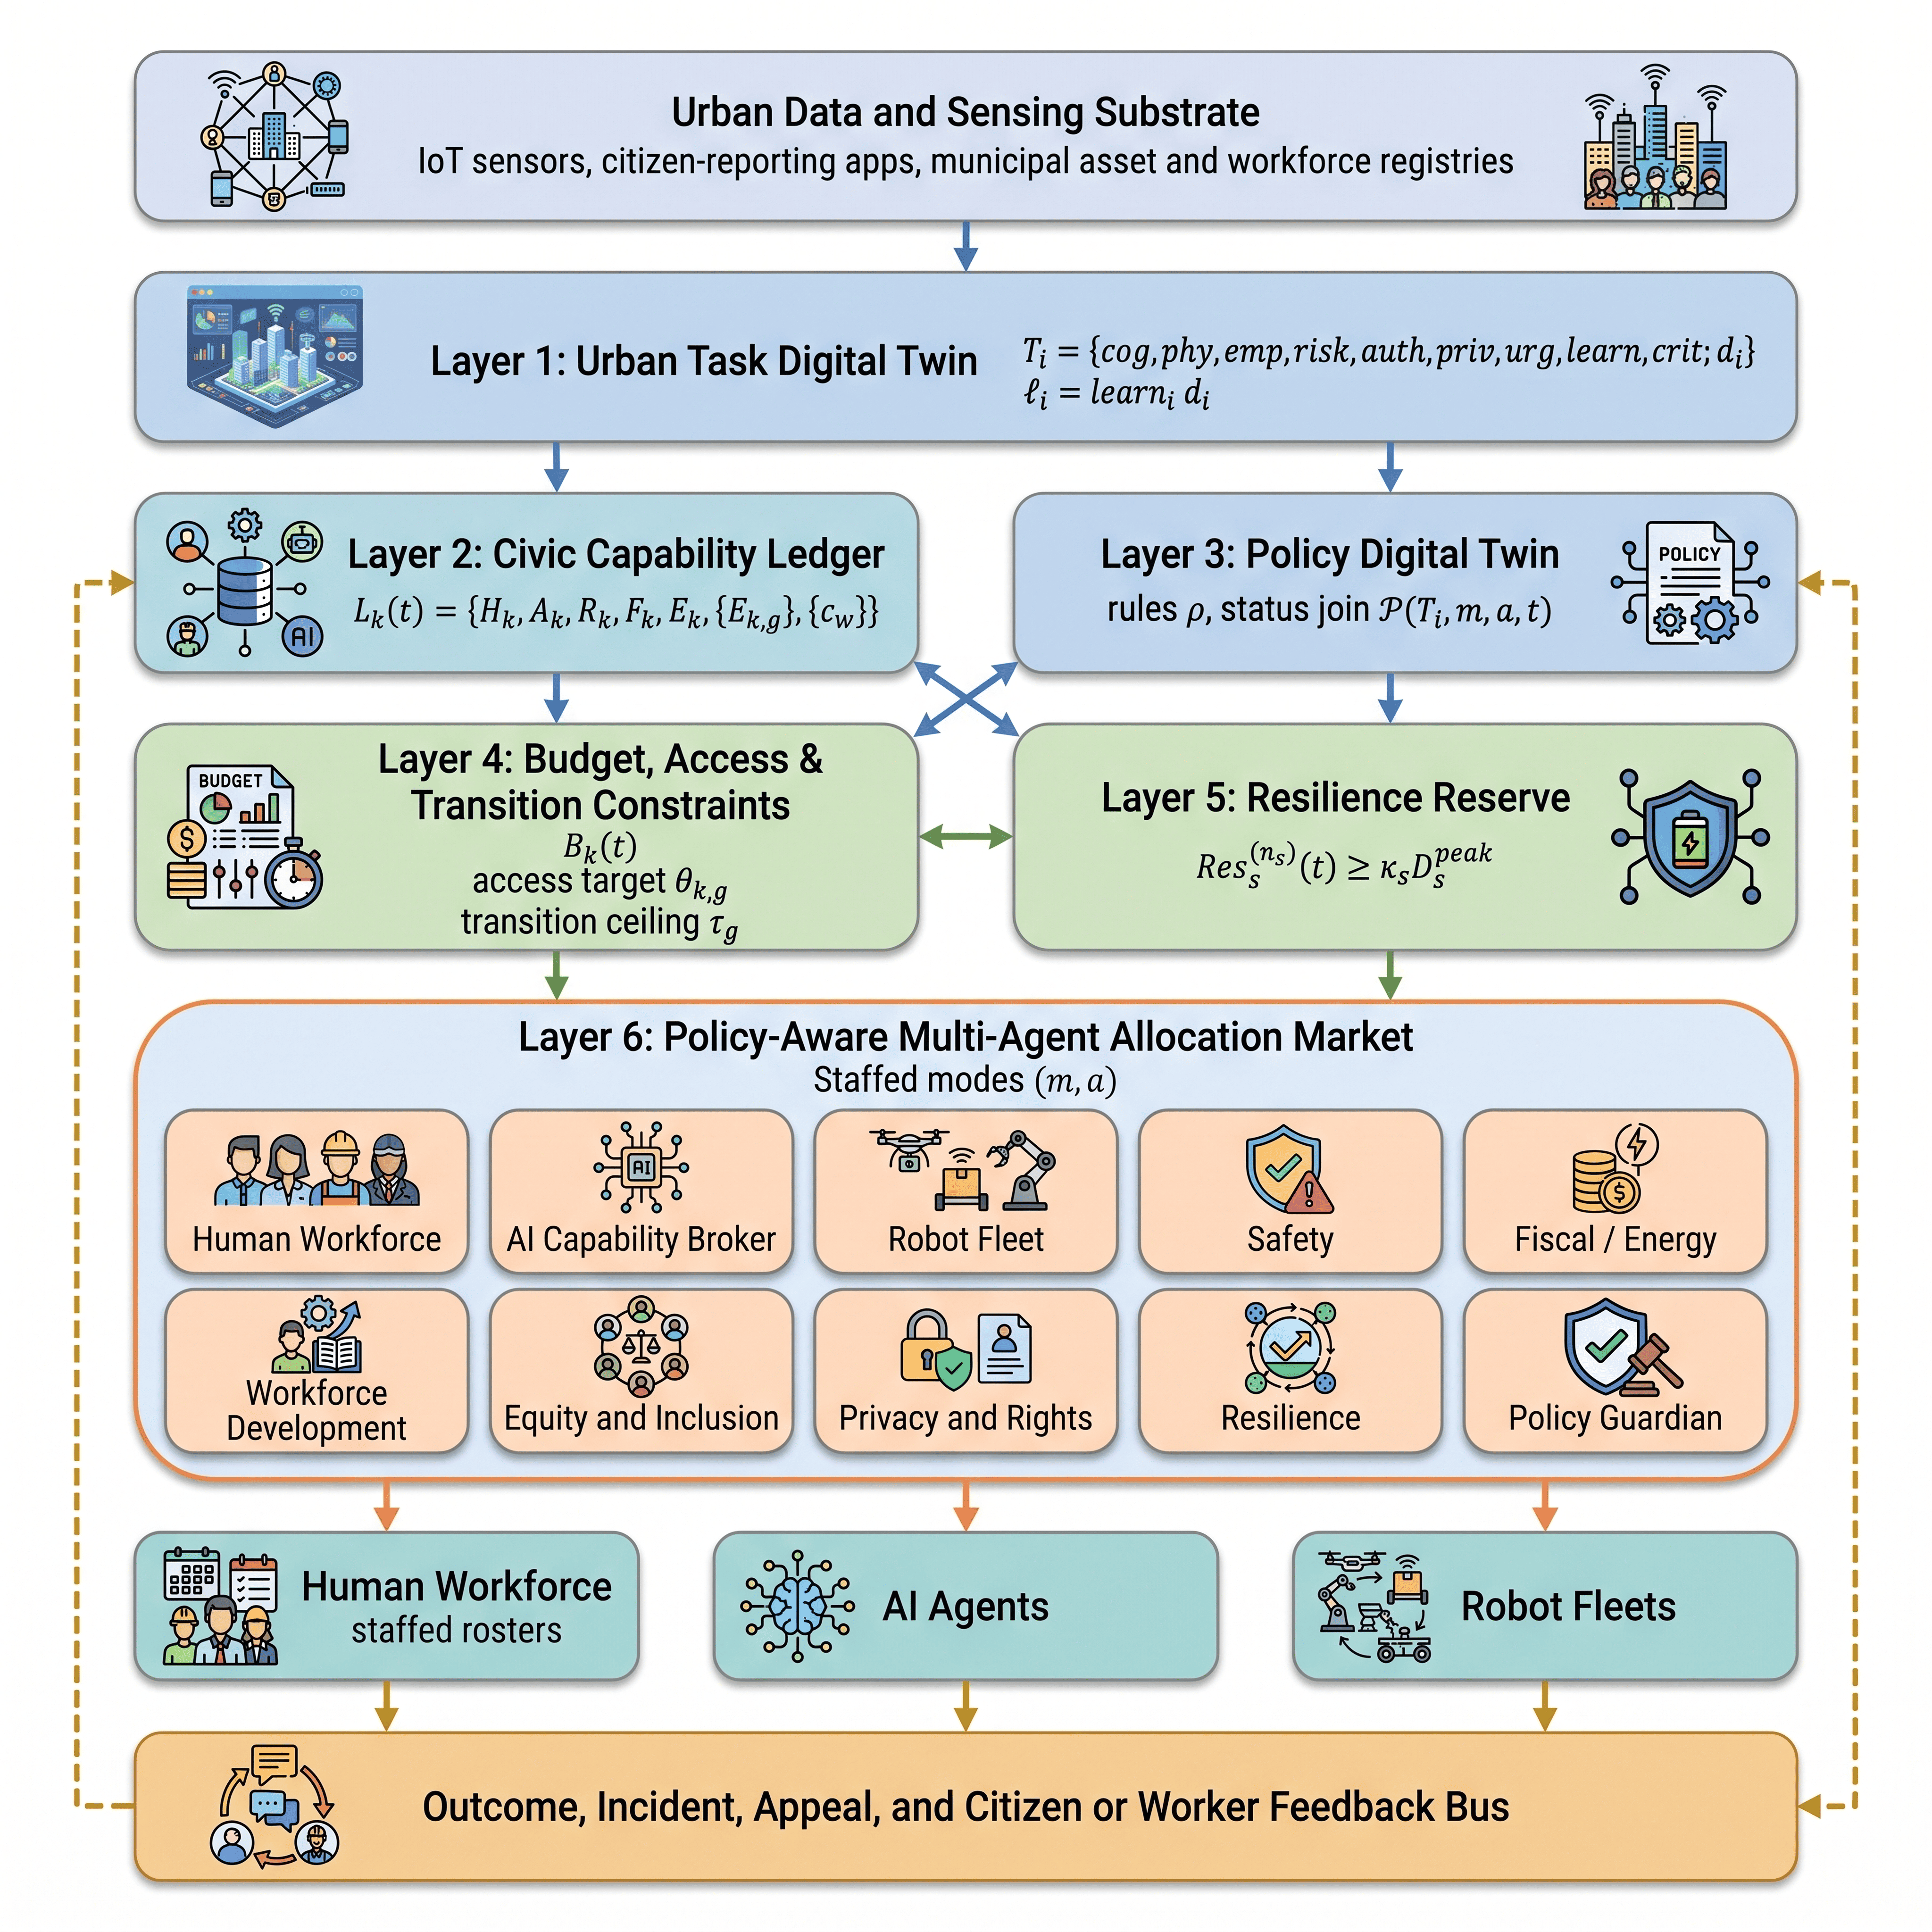
\includegraphics[width=\linewidth]{images/arch}
		\caption{Reference architecture of CivicWorkOS, read top to bottom. Solid arrows are the forward allocation path from sensed urban data through the governance layers to execution; the ten agents are drawn inside the market because they constitute it. The Ledger supplies fallback capacity $F_k$ of Equation~\eqref{eq:fallback} to the reserve through Equation~\eqref{eq:cs}, and per-practitioner practice totals $c_w$ to the career-stage test of Equation~\eqref{eq:stage}. The Policy Twin supplies the replacement factor $\eta_k$, the access target $\theta_{k,g}$, and the roster guards that restrict $\mathcal{A}_{i,m}$. Dashed arrows are the outcome-feedback path, which updates both governance services.}
		\label{fig:architecture}
	\end{figure}
	
	\subsection{Runtime Allocation Workflow}
	\label{sec:workflow}
	
	Figure~\ref{fig:workflow} shows the per-task control flow that Algorithm~\ref{alg:scv} formalizes: encode the task, query the policy twin per mode, build and prune the roster set according to the returned status, price each surviving staffed mode by~\eqref{eq:cad} and~\eqref{eq:scv}, apply the admissibility test of Section~\ref{sec:online}, and execute the arg max on the Lagrangian-augmented score. Three properties matter. Policy filtering is per mode and roster pruning is per roster, as~\eqref{eq:policy} and the \textit{restrict} status require. Either stage may empty the candidate set, in which case the task routes to Zone Z4 human-reserved execution rather than leaving the arg max undefined, and that event is counted, because its rate is the operational price of the constraint system and is one of the metrics the protocol of Appendix~\ref{app:protocol} requires to be reported. And the ledger update writes both the domain accrual $\Lambda_k$ and the per-practitioner totals $c_w$, since only the second can move a practitioner across the career-stage boundary of~\eqref{eq:stage}.
	
	\begin{figure}[!htbp]
		\centering
		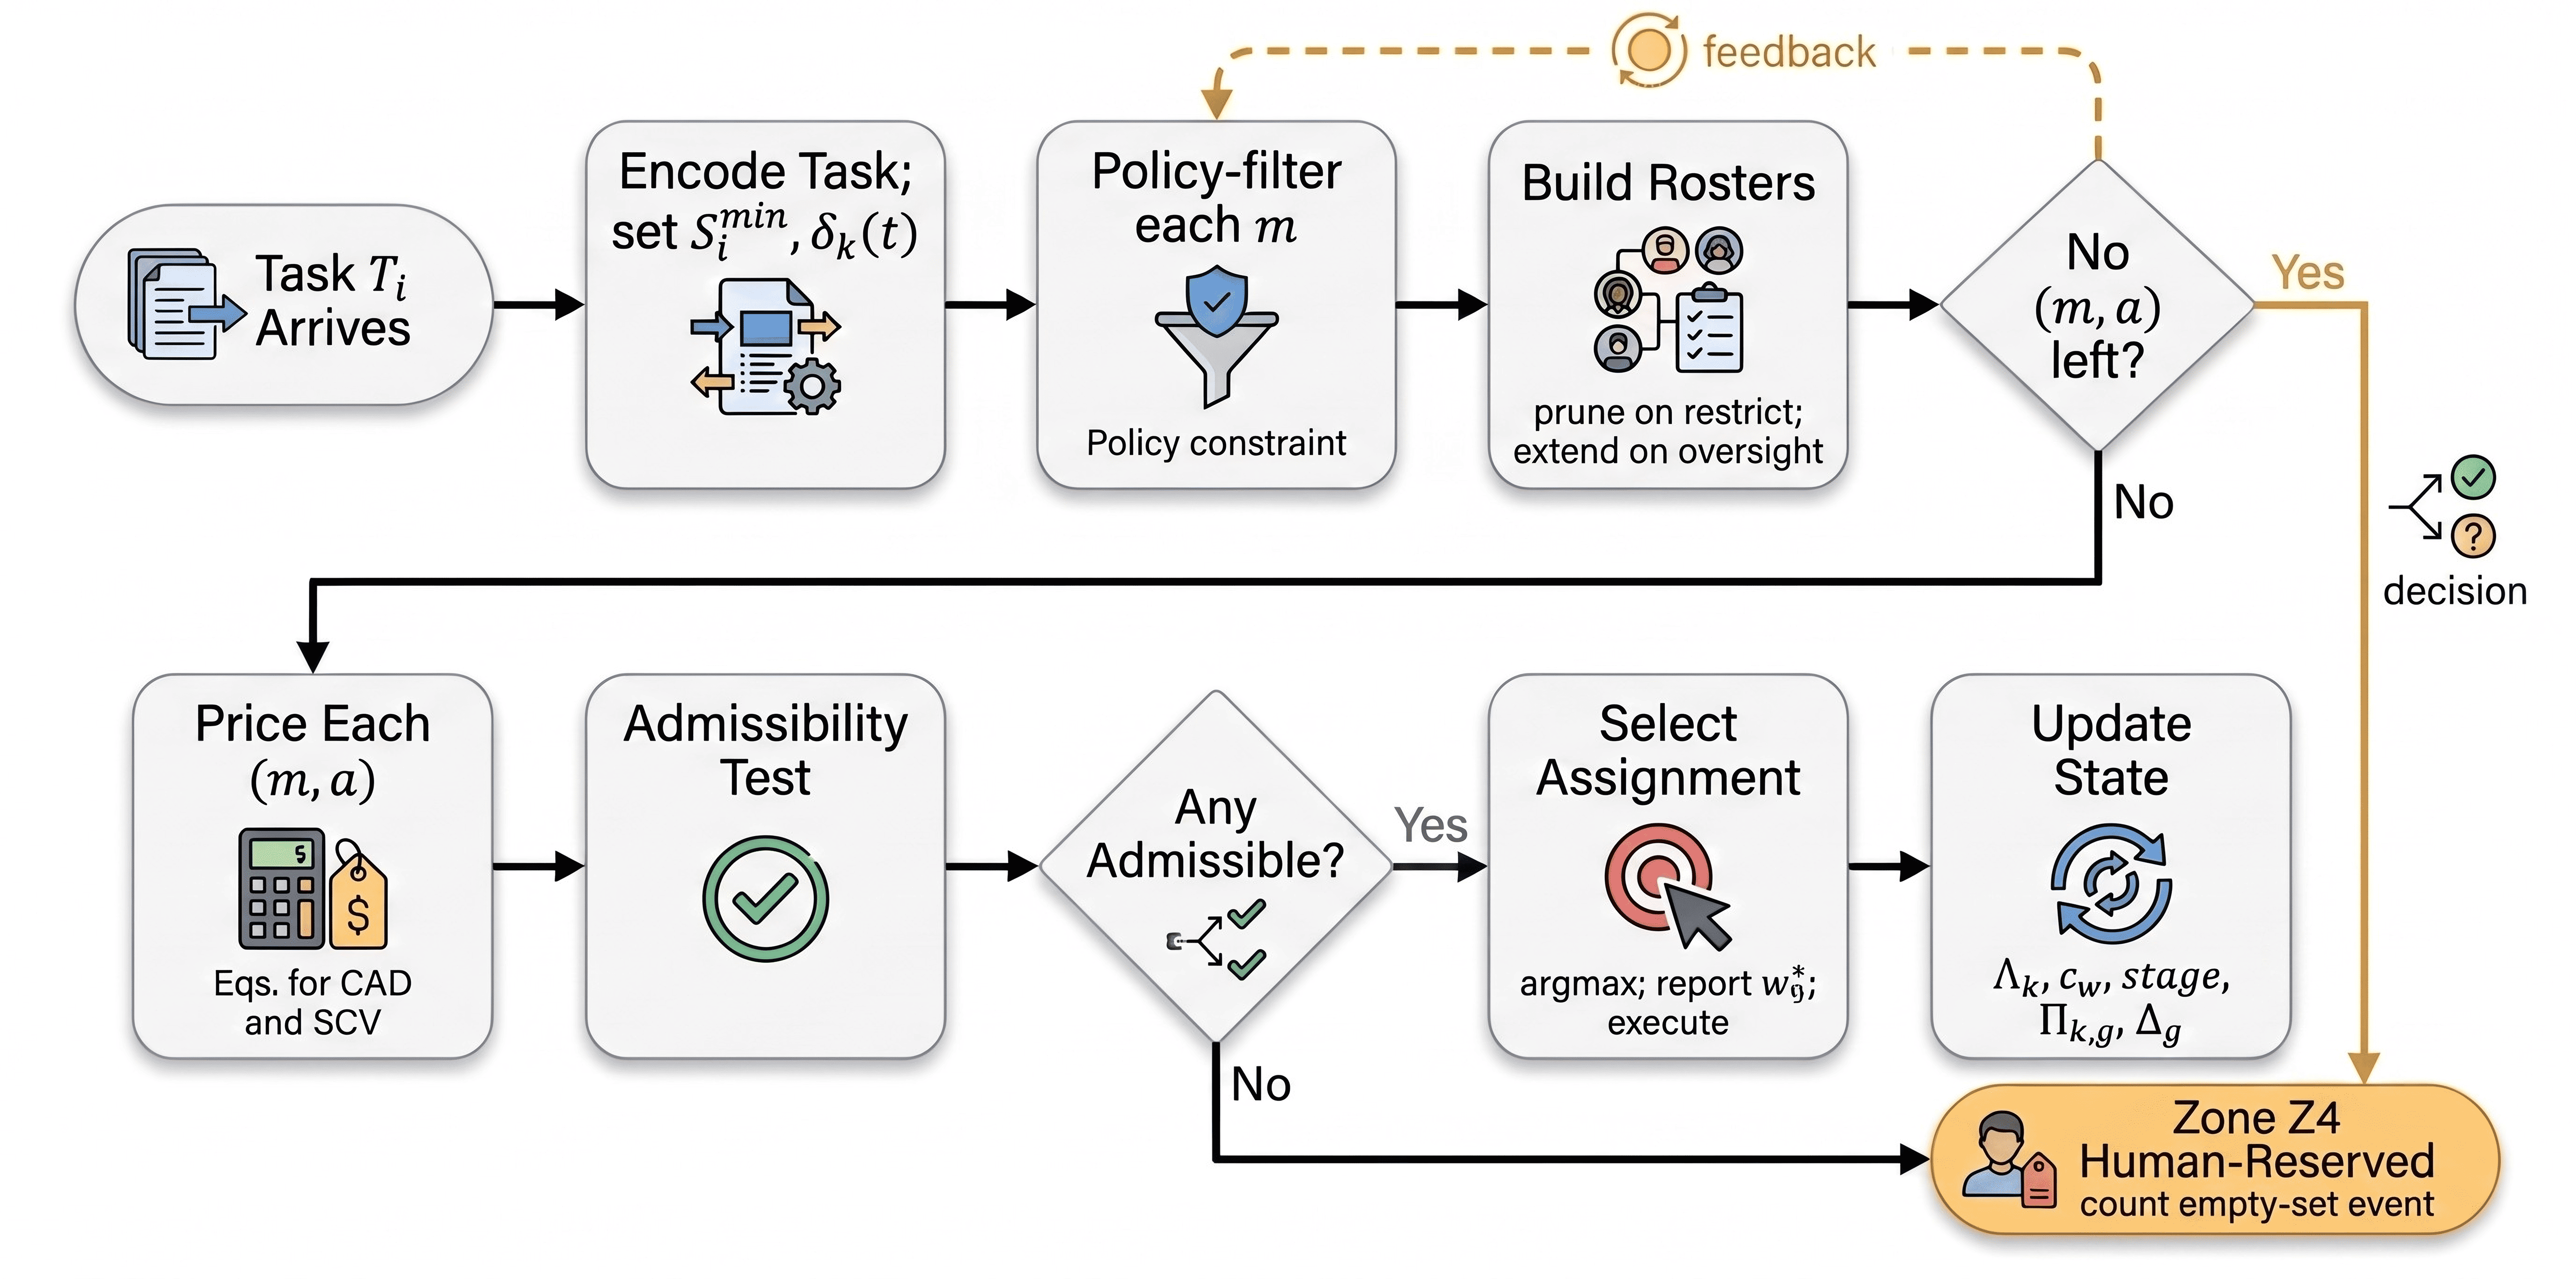
\includegraphics[width=\linewidth]{images/runtime}
		\caption{Runtime allocation workflow, matching Algorithm~\ref{alg:scv}. The upper row encodes the task, sets the safety floor and the catch-up increment, policy-filters modes, and builds the roster set, pruning it where the twin returns \textit{restrict} and extending it with a named reviewer where it returns \textit{allow-with-oversight}. The lower row prices the surviving staffed modes, applies the admissibility test~\eqref{eq:admis}, and either falls back to Zone Z4 or selects and executes. The dashed edge returns outcomes to the Policy Digital Twin, which is what makes the zone-transition predicates (Section~\ref{sec:zones}) evaluable.}
		\label{fig:workflow}
	\end{figure}
	
	\subsection{Sustainable Civic Value (SCV)}
	\label{sec:math}
	
	For each task $T_i$ and staffed mode $(m,a)$, the \textit{Sustainable Civic Value} is given by equation~\eqref{eq:scv}:
	\begin{equation}
		\begin{split}
			SCV_{i,m,a} =\;&
			w_1 Q_{i,m,a}
			+w_2 S_{i,m,a}
			+w_3 P_{i,m,a}
			+w_4 Eq^{srv}_{i,m,a}
			+w_5 Tr_{i,m,a}\\
			&-w_6 Cost_{i,m,a}
			-w_7 En_{i,m}
			-w_8 Pr_{i,m}
			-w_9 CAD_{i,m,a},
		\end{split}
		\label{eq:scv}
	\end{equation}
	where $Q$ is service quality, $S$ safety, $P$ productivity, $Eq^{srv}$ the equity of service delivery across resident groups and districts, $Tr$ agent trust, $Cost$ operating cost, $En$ energy use, $Pr$ privacy risk, and $CAD$ the debt of~\eqref{eq:cad}. The first eight terms are flows measured on the task's execution window, and the ninth is a change in municipal stocks. Six terms depend on the roster as well as the mode, because staffing a developing practitioner alongside a competent lead changes the quality, safety, productivity, trust, and cost of the execution as well as its developmental content. Section~\ref{sec:problem} argued why no capability-formation, resilience-contribution, or accountability term appears separately, and Section~\ref{sec:weights} reports the effective weight each civic construct receives once $w_9$ and the debt weights are composed.
	
	Weighting a multi-criteria score linearly trades flexibility for interpretability and tractability relative to explicit Pareto-front methods~\cite{Osika2023,ZhengRasheed2026}. One consequence must be stated here rather than deferred, because it bears on the democratic claims of Section~\ref{sec:feedback}. A linear scalarization recovers only solutions on the convex hull of the attainable set, so allocations in non-convex regions of the Pareto frontier are unreachable for \textit{every} weight vector~\cite{Osika2023}. If a socially preferred compromise lies in such a region, no deliberation over $w_1,\ldots,w_9$ can select it, and the panel would be exercising authority over a strictly smaller set of outcomes than it appears to. Section~\ref{sec:limitations} records this restriction with the alternatives that would remove it.
	
	\subsubsection*{Normalization}
	
	The nine terms have incompatible native units, so each is rescaled to $[0,1]$ before weighting, and the two families are rescaled differently. For the eight \textit{flow} terms we use min--max normalization against a trailing twelve-month, sector-specific window, refreshed so the scale adapts as practice improves. That would be wrong for the debt components: if $D^{skill}$ and $D^{fall}$ were normalized against a rolling window, then as the pipeline decayed the reference range would decay with it, normalized scores would stay comfortably mid-range, and a framework premised on a city looking efficient while its capability empties out would have built an instrument that cannot see the emptying.
	
	The five debt components therefore carry no windowed normalization at all. Each is constructed as a ratio whose denominator is fixed externally, which places each debt term in $[0,1]$ as defined in equation~\eqref{eq:anchors}:
	\begin{equation}
		\begin{aligned}
			D^{skill}_{i,m,a} &= 1-\phi_m\psi_a &&\text{against the task's own full developmental content } \ell_i,\\
			D^{fall}_{i,m} &= \min\!\Big(1,\ \Delta F_{\kappa(i)}(m)\,/\,\rho_{\sigma(i)}\Big) &&\text{against the statutory reserve } \rho_s=\kappa_s D^{peak}_s,\\
			D^{acct}_{i,m} &= crit_i \cdot n^{unacct}_{i,m}/n^{steps}_{i,m} &&\text{against the decision-step count of the task},\\
			D^{dep}_{i,m} &= n^{single}_{i,m}/n^{auto}_{i,m} &&\text{against the automated-input count of the mode},\\
			D^{trans}_{i,m} &= \textstyle\sum_{g}\varpi_{g}(i,m)\,\bigl(1-\chi_g\bigr) &&\text{against funded transition coverage } \chi_g,
		\end{aligned}
		\label{eq:anchors}
	\end{equation}
	where $\Delta F_k(m)$ is the fallback reduction mode $m$ would cause if generalized across the domain and $\varpi_g(i,m)$ is group $g$'s share of the workers whose allocated hours the mode reduces. All five denominators are external to observed performance, so a decade of decline registers as a decade of decline. Note that $D^{trans}$ is anchored to the reskilling coverage $\chi_g$ and not to the displacement ceiling $\tau_g$: the ceiling is a hard constraint on $\Delta_g$, and the priced quantity is the unfunded share of the burden.

	\subsubsection*{Default Weights and What They Actually Carry}
	\label{sec:weights}

	The illustrative CivicWorkOS weights, summing to one, are $w_1{=}0.15$ (quality), $w_2{=}0.18$ (safety), $w_3{=}0.14$ (productivity), $w_4{=}0.10$ (service equity), $w_5{=}0.05$ (trust), $w_6{=}0.08$ (cost), $w_7{=}0.03$ (energy), $w_8{=}0.05$ (privacy risk), and $w_9{=}0.22$ (Civic Automation Debt). The debt weights are $\alpha{=}0.28$ (skill formation), $\beta{=}0.22$ (fallback), $\gamma{=}0.18$ (accountability), $\delta{=}0.12$ (dependency), and $\epsilon{=}0.20$ (transition burden), also summing to one. These are design defaults for the panel of Section~\ref{sec:feedback} to revise, not fitted estimates. Appendix~\ref{app:protocol} (Table~\ref{tab:app-params}) assigns a default to every remaining parameter in the framework, because a framework that names a dozen policy parameters and assigns values to two is not implementable.

	Because a weight vector can assert a priority the arithmetic then withholds, Table~\ref{tab:weights} reports the \textit{effective} weight each construct carries once $w_9$ and the debt weights are composed. Three things are visible there. The deferred block carries 0.22 in total, the largest single block and more than productivity at 0.14, though not the largest single construct, which is safety at 0.180. Any statement that Civic Automation Debt carries the largest weight in this objective is true of the block and false of every one of its components, and we make the distinction because an earlier version of this article's abstract did not. No individual debt component outweighs a major operational term, with skill formation at 0.062 sitting between cost and trust, since a framework claiming that capability erosion dominates every other consideration would be unusable. And labor-transition burden carries 0.044. For a question about labor transition that number invites scrutiny, so we give the reasoning: an objective weight is a quantity other terms can outvote, and transition is therefore also carried by the hard constraint~\eqref{eq:justtransition}, which they cannot. Where a city judges 0.044 too low the panel raises it; where a city judges displacement unacceptable at any weight it lowers $\tau_g$ instead. Placing the strong lever in the constraint and the weak one in the objective is the design, and Proposition~\ref{prop:price} is how a city checks which of the two is actually deciding.

	\begin{table}[!htbp]
		\caption{Effective weight of each construct in the CivicWorkOS default configuration, obtained by composing $w_9=0.22$ with the debt weights. The deferred block is the largest single block of the objective; safety is the largest single construct. Column sums to 1.000.}
		\label{tab:weights}
		\begin{tabular}{@{}llc@{}}
			\toprule
			\textbf{Construct} & \textbf{Enters via} & \textbf{Effective weight}\\
			\midrule
			Safety & $w_2$ & 0.180\\
			Service quality & $w_1$ & 0.150\\
			Productivity & $w_3$ & 0.140\\
			Service equity (residents) & $w_4$ & 0.100\\
			Operating cost & $w_6$ & 0.080\\
			Skill formation & $w_9\alpha$ & 0.062\\
			Trust & $w_5$ & 0.050\\
			Privacy risk & $w_8$ & 0.050\\
			Fallback capacity & $w_9\beta$ & 0.048\\
			Labor-transition burden (workers) & $w_9\epsilon$ & 0.044\\
			Accountability & $w_9\gamma$ & 0.040\\
			Energy & $w_7$ & 0.030\\
			Vendor dependency & $w_9\delta$ & 0.026\\
			\midrule
			\textit{Deferred block total} & $w_9$ & \textit{0.220}\\
			\bottomrule
		\end{tabular}
	\end{table}

	\subsection{The City-Wide Allocation Program}
	\label{sec:program}
	
	The constraints of Sections~\ref{sec:hcpb} through~\ref{sec:layer5} couple decisions across tasks: whether one inspection may go to an unstaffed autonomous team depends on how much practice the domain's other inspections have already delivered, and to whom. A per-task rule cannot by itself guarantee feasibility, so the program it approximates must be written down. Over a rebalancing window containing task set $\mathcal{T}(\Delta T)$, CivicWorkOS solves the program formulated in equation~\eqref{eq:program} (with objective~\eqref{eq:prog-obj} and constraints~\eqref{eq:prog-assign}--\eqref{eq:prog-cap}):
	\begin{subequations}
		\label{eq:program}
		\begin{align}
			\max_{\mathbf{x},\boldsymbol{\varsigma}} \quad & \sum_{i \in \mathcal{T}(\Delta T)} \sum_{m \in \mathcal{M}} \sum_{a\in\mathcal{A}_{i,m}} x_{i,m,a}\, SCV_{i,m,a} \;-\; M \sum_{k,g}\varsigma_{k,g}
			\label{eq:prog-obj}\\
			\text{s.t.}\quad
			& \textstyle\sum_{m} \sum_{a} x_{i,m,a} = 1, && \forall i,
			\label{eq:prog-assign}\\
			& x_{i,m,a} = 0 \ \text{ if } \mathcal{P}(T_i,m,a,t)=\textit{prohibit},
			\label{eq:prog-policy}\\
			& x_{i,m,a} = 0 \ \text{ if } S_{i,m,a} < S^{min}_i,
			\label{eq:prog-safety}\\
			& \textstyle\sum_{i \in \mathcal{T}_k} \sum_{m}\sum_{a} x_{i,m,a}\,\ell_i\,\phi_m\,\psi_a \geq B_k(t), && \forall k,
			\label{eq:prog-hcpb}\\
			& \Pi_{k,g}(\mathbf{x}) + \varsigma_{k,g} \geq \theta_{k,g} - \varepsilon_k, \quad \varsigma_{k,g}\geq 0, && \forall k,g,
			\label{eq:prog-access}\\
			& \Delta_g(\mathbf{x}) \leq \tau_g, && \forall g,
			\label{eq:prog-just}\\
			& Res^{(n_s)}_s(\mathbf{x}) \geq \kappa_s D^{peak}_s, && \forall s,
			\label{eq:prog-res}\\
			& \textstyle\sum_{i}\sum_{m}\sum_{a} x_{i,m,a}\, u_{i,m,a,r} \leq U_r, && \forall r,
			\label{eq:prog-cap}\\
			& x_{i,m,a} \in \{0,1\}.
			\label{eq:prog-int}
		\end{align}
	\end{subequations}
	Here $u_{i,m,a,r}$ is the consumption of resource $r$ (human hours by grade and stage, robot-fleet hours by class, AI inference budget) that staffed mode $(m,a)$ implies for task $i$, and $U_r$ its availability. The access constraint~\eqref{eq:prog-access} carries an elastic slack $\varsigma_{k,g}$ penalized at a large $M$ in the objective, so an unattainable composition target degrades into a published shortfall rather than into infeasibility, and no individual assignment is ever compelled by the target alone. Section~\ref{sec:legality} explains why that elasticity is a legal requirement and not only a numerical convenience. The roster dimension is what makes~\eqref{eq:prog-cap} bind on individual practitioners rather than on an anonymous pool, and it is what makes~\eqref{eq:prog-access} evaluable at all. Program~\eqref{eq:program} is a binary multi-dimensional assignment problem with side constraints, NP-hard in general, since it reduces to a generalized assignment problem when only~\eqref{eq:prog-cap} binds. This is why the framework solves it periodically over a window rather than continuously. Where the window size stops being tractable is an empirical question about a particular solver and a particular city, and Appendix~\ref{app:protocol} specifies the profile that would answer it; we have not measured one, and this article makes no scalability claim.
	
	\subsection{Online Allocation, Duals, and the Admissibility Test}
	\label{sec:online}
	
	Between rebalances, tasks arrive one at a time and must be decided immediately, so CivicWorkOS approximates~\eqref{eq:program} online by Lagrangian relaxation of \textit{all five} coupling constraints. Let $\lambda_k, \mu_s, \nu_{k,g}, \varrho_g, \upsilon_r \geq 0$ be the dual prices of~\eqref{eq:prog-hcpb},~\eqref{eq:prog-res},~\eqref{eq:prog-access},~\eqref{eq:prog-just}, and~\eqref{eq:prog-cap} from the most recent solution. The online score is defined in equation~\eqref{eq:aug}:
	\begin{equation}
		\begin{split}
			\widetilde{SCV}_{i,m,a} = SCV_{i,m,a}
			&+ \lambda_{\kappa(i)}\,\ell_i\,\phi_m\,\psi_a
			+ \mu_{\sigma(i)}\,\Delta^{res}_{\sigma(i)}(m,a)
			+ \sum_{g}\nu_{\kappa(i),g}\,\ell_i\,\phi_m\,\psi_a\,\pi^{dev}_{a,g}\\
			&- \sum_{g}\varrho_g\,\delta^{disp}_g(i,m,a)
			- \sum_{r}\upsilon_r\,u_{i,m,a,r} .
		\end{split}
		\label{eq:aug}
	\end{equation}
	Earlier presentations priced only the first three, leaving the framework blind between rebalances to the very displacement it exists to bound and free to assign more human hours than the city has humans. The last two terms close that gap, and the corresponding brackets in~\eqref{eq:admis} bound the residual violation by Proposition~\ref{prop:violation}.
	
	The resilience term requires a definition that a single task can satisfy. One task's mode choice does not change a robot fleet's capacity, so $\Delta^{res}$ is defined counterfactually in equation~\eqref{eq:deltares} and scaled by the task's share of service demand:
	\begin{equation}
		\Delta^{res}_s(m,a) \;=\; \frac{d_i}{D^{tot}_s(\Delta T)}\,
		\Bigl[\,Res^{(n_s)}_s\bigl(t \,\big|\, (m,a) \text{ generalized across } s\bigr) - Res^{(n_s)}_s(t)\,\Bigr],
		\label{eq:deltares}
	\end{equation}
	where $D^{tot}_s(\Delta T)$ is the service's total task-hours in the window. The Resilience Agent maintains the mode-to-capacity map that makes the counterfactual computable, and the scaling makes the per-task term additive across the window so that summing~\eqref{eq:deltares} over the service's tasks recovers the policy-level change.
	
	\subsubsection*{Duals from a Binary Program}
	
	Program~\eqref{eq:program} is integral, and integer programs have no exact duals. We take $\lambda,\mu,\nu,\varrho,\upsilon$ from the LP relaxation solved at the root node, which is a valid subgradient of the relaxed value function and the standard construction for Lagrangian decomposition of assignment problems. The consequence is that~\eqref{eq:aug} approximates the relaxed rather than the integral program, and the approximation error is bounded by the integrality gap, which the solver reports at each rebalance and which the protocol of Appendix~\ref{app:protocol} requires to be tabulated at every cadence. In the worked case of Section~\ref{sec:worked} that gap is $7.8\times10^{-6}$ objective units per task, because a single coupling constraint plus the simplex constraint admits at most two active staffed modes at an LP vertex and the domain's task count is large enough that rounding costs almost nothing. We do not claim this holds at every scale, and the reported gap is the diagnostic that says when it stops holding.
	
	\subsubsection*{The Admissibility Test}
	
	Constraints~\eqref{eq:prog-hcpb} and~\eqref{eq:prog-res} concern the state of a domain or service, not of a staffed mode, so testing them as written inside a loop over $(m,a)$ removes either every candidate or none. Worse, a city currently \textit{below} threshold would have every candidate removed and every task routed to human-reserved execution, including the machine-assisted allocations that free the human capacity needed to climb back above threshold, so the framework would fail hardest in exactly the state it exists to prevent. We therefore evaluate the constraints on the evaluated post-execution state and add a feasibility-restoration branch. Staffed mode $(m,a)$ is \textit{admissible} for task $i$ at time $t$ if it satisfies equation~\eqref{eq:admis}:
	\begin{equation}
		\begin{aligned}
			&\mathcal{P}(T_i,m,a,t) \neq \textit{prohibit}
			\quad\text{and}\quad S_{i,m,a} \geq S^{min}_i, \quad\text{and}\\[2pt]
			&\Bigl[\,Res^{(n_s)}_s(t^{+}\!\mid\! m,a) \geq \rho_s \ \ \text{or}\ \ \bigl(Res^{(n_s)}_s(t) < \rho_s \ \wedge\ \Delta^{res}_s(m,a) \geq 0\bigr)\Bigr], \quad\text{and}\\[2pt]
			&\Bigl[\,\Lambda_k(t^{+}\!\mid\! m,a) \geq \bar{B}_k(t) \ \ \text{or}\ \ \ell_i\,\phi_m\,\psi_a \;\geq\; \delta_k(t)\Bigr], \quad\text{and}\\[2pt]
			&\Delta_g\bigl(t^{+}\!\mid\! m,a\bigr) \leq \tau_g \ \ \forall g,
			\quad\text{and}\quad
			u_{i,m,a,r} \leq U_r - U^{used}_r(t) \ \ \forall r,
		\end{aligned}
		\label{eq:admis}
	\end{equation}
	with $s=\sigma(i)$, $k=\kappa(i)$, where $\Lambda_k(t)$ is the practice accrued in domain $k$ so far in the current budget period, $\bar{B}_k(t) = B_k(t)\cdot t/\Delta T$ the pro-rated budget trajectory, and the catch-up threshold $\delta_k(t)$ is defined in equation~\eqref{eq:catchup}:
	\begin{equation}
		\delta_k(t) \;=\; \frac{\max\bigl(0,\ B_k(t)-\Lambda_k(t)\bigr)}{n^{rem}_k(t)}
		\label{eq:catchup}
	\end{equation}
	the per-task developmental increment required to close the remaining gap over the $n^{rem}_k(t)$ tasks the domain still expects in the period. The catch-up threshold~\eqref{eq:catchup} is the second substantive repair in this section. A restoration branch that admits any staffed mode with $\phi_m\psi_a > 0$ would let a domain that has fallen behind stay behind indefinitely, allocating every task to the lowest positive developmental credit and passing the test every time. Requiring $\ell_i\phi_m\psi_a \geq \delta_k(t)$ instead means the mode must carry its share of the shortfall, and as the gap grows the test becomes strictly more demanding, which is the behavior the prose always claimed and the formula did not deliver.
	
	The allocation $(m,a)^\ast_i$ is then determined by equation~\eqref{eq:argmax}:
	\begin{equation}
		(m,a)^{\ast}_i = \arg\max_{(m,a) \in \mathcal{A}(i,t)} \widetilde{SCV}_{i,m,a},
		\label{eq:argmax}
	\end{equation}
	over the admissible set $\mathcal{A}(i,t)$, with the Zone Z4 fallback when $\mathcal{A}(i,t)=\emptyset$. After execution, outcomes are folded back into policy through equation~\eqref{eq:feedback}:
	\begin{equation}
		Policy_{t+1} =
		f\bigl(Policy_t,\,Performance_t,\,Incidents_t,\,CAD_t,\,Distribution_t,\,Feedback_t\bigr),
		\label{eq:feedback}
	\end{equation}
	discussed in Section~\ref{sec:feedback} as the closed governance loop. Algorithm~\ref{alg:scv} states the per-task procedure, including the roster construction and the two intermediate policy statuses that earlier presentations described but never implemented.
	
	\begin{algorithm}[H]
		\caption{Online policy-aware allocation over staffed modes}
		\label{alg:scv}
		\begin{algorithmic}[1]
			\Require Task $T_i$; time $t$; ledger $L(t)$; policy twin $\mathcal{P}$; budgets $B(t)$; thresholds $\rho$; duals $\lambda,\mu,\nu,\varrho,\upsilon$ from the last solution of~\eqref{eq:program}
			\Ensure Selected staffed mode $(m,a)^\ast_i$
			\State Encode $T_i$ via~\eqref{eq:task}; $\ell_i \gets learn_i d_i$; $s \gets \sigma(i)$; $k \gets \kappa(i)$; $S^{min}_i \gets risk_i\,crit_i$
			\State $\mathcal{A} \gets \emptyset$; $\delta_k \gets$~\eqref{eq:catchup}
			\For{each $m \in \mathcal{M}$}
			\State $z \gets \mathcal{P}(T_i,m,\cdot,t)$ evaluated on the mode-level rules \Comment{join of~\eqref{eq:lattice}}
			\If{$z = \textit{prohibit}$} \State \textbf{continue} \EndIf
			\State $\mathcal{A}_{i,m} \gets$ feasible rosters for $m$ from available $w\in\mathcal{W}_k$, with $\psi_a$ by~\eqref{eq:psi}, $\pi^{dev}_{a,g}$ by~\eqref{eq:groupshare}
			\If{$z = \textit{restrict}$} \State prune $\mathcal{A}_{i,m}$ to rosters satisfying the firing rules' roster guards \EndIf
			\If{$z = \textit{allow-with-oversight}$} \State append the named reviewer to each roster; add reviewer time to $Cost$; raise $\phi_m$ by the assessed retained-judgment share \EndIf
			\For{each $a \in \mathcal{A}_{i,m}$}
			\State Query the ten agents for $Q,S,P,Eq^{srv},Tr,Cost,En,Pr$ and $D^{skill},D^{fall},D^{acct},D^{dep},D^{trans}$
			\State $CAD_{i,m,a} \gets$~\eqref{eq:cad}; \ $SCV_{i,m,a} \gets$~\eqref{eq:scv}; \ $\Delta^{res}_s(m,a) \gets$~\eqref{eq:deltares}
			\If{$(m,a)$ satisfies~\eqref{eq:admis}}
			\State $\widetilde{SCV}_{i,m,a} \gets$~\eqref{eq:aug}; \ $\mathcal{A} \gets \mathcal{A}\cup\{(m,a)\}$
			\EndIf
			\EndFor
			\EndFor
			\If{$\mathcal{A} = \emptyset$}
			\State $(m,a)^\ast_i \gets$ Zone Z4 human-reserved roster; record the empty-set event; update $L(t)$; \Return
			\EndIf
			\State $(m,a)^\ast_i \gets \arg\max_{(m,a) \in \mathcal{A}} \widetilde{SCV}_{i,m,a}$ \Comment{Equation~\eqref{eq:argmax}}
			\State Report $w_9^\star(i)$ by Proposition~\ref{prop:price} to the allocation record
			\State Execute; observe outcomes; $\Lambda_k \gets \Lambda_k + \ell_i \phi_{m^\ast}\psi_{a^\ast}$
			\State For each $w \in a^\ast$: $c_w \gets c_w + \ell_i \phi_{m^\ast}\omega_{a^\ast,w}$; re-evaluate $\mathrm{stage}_k(w,t)$ by~\eqref{eq:stage}
			\State Update $L(t{+}1)$, accumulated CAD, $\Pi_{k,g}$, $\Delta_g$, $U^{used}_r$; emit to the feedback bus via~\eqref{eq:feedback}
		\end{algorithmic}
	\end{algorithm}
	
	Per task, Algorithm~\ref{alg:scv} performs at most $|\mathcal{M}|=7$ policy queries and $\sum_m |\mathcal{A}_{i,m}|$ agent estimates, so the online decision scales linearly in the arrival rate and in the roster count. The periodic solution of~\eqref{eq:program}, not the online loop, is the scalability bottleneck. The relationship between the two is standard for Lagrangian decomposition: the online rule is exact when the duals are exact and the window short enough that the state has not drifted, and degrades as either assumption weakens, which is why the rebalance cadence is a tunable parameter and why Appendix~\ref{app:protocol} requires the tracking gap to be measured across cadences rather than assumed.
	
	\subsection{Feasibility of the Capability Budget and the Intake Requirement}
	\label{sec:feasibility}
	
	A capability budget that the task stream cannot supply is not a demanding constraint, it is an infeasible one, and a framework that does not say when this happens will report a failure of its own arithmetic as a failure of the city. We therefore state the condition and the response.
	
	\begin{Proposition}[Feasibility of the capability budget]
		\label{prop:feasibility}
		Let $\Phi_k(\Delta T)=\sum_{i\in\mathcal{T}_k(\Delta T)}\ell_i$ be the domain's total developmental content in the period, and let
		\begin{equation*}
			\bar\zeta_k \;=\; \max\bigl\{\phi_m\psi_a \;:\; (m,a) \text{ admissible for some } i\in\mathcal{T}_k\bigr\}
		\end{equation*}
		be the largest developmental credit any admissible staffed mode delivers. Then equation~\eqref{eq:hcpb} is satisfiable only if the condition in equation~\eqref{eq:feas} holds:
		\begin{equation}
			B_k(t) \;\leq\; \Phi_k(\Delta T)\,\bar\zeta_k .
			\label{eq:feas}
		\end{equation}
		Where the estimator~\eqref{eq:hcpb-estimator} is attained by its second argument, this is equivalent to a ceiling on attrition given by equation~\eqref{eq:rcrit}:
		\begin{equation}
			r_k(t) \;\leq\; r^{crit}_k \;=\; \frac{\Phi_k(\Delta T)\,\bar\zeta_k}{\eta_k\,N_k(t)\,h_k},
			\label{eq:rcrit}
		\end{equation}
		and symmetrically to ceilings on $\eta_k$ and $h_k$ and a floor on the task volume.
	\end{Proposition}
	
	\begin{proof}
		Every term of the left side of~\eqref{eq:hcpb} is bounded above by $\ell_i\bar\zeta_k$, and~\eqref{eq:prog-assign} selects exactly one staffed mode per task, so $\Lambda_k \leq \bar\zeta_k\sum_i \ell_i = \Phi_k\bar\zeta_k$. Substituting~\eqref{eq:hcpb-estimator} and solving for $r_k$ gives~\eqref{eq:rcrit}.
	\end{proof}
	
	Three things make~\eqref{eq:feas} bind harder than it first appears. $\bar\zeta_k$ is a product of two factors below one, so machine assistance and supervision ratios both reduce it. The safety floor $S^{min}_i$ and the policy twin's roster guards remove exactly the high-$\phi_m$ candidates on the tasks where the budget most wants them, since unaided human work on a hazardous task is what a safety floor is for. And $\bar\zeta_k$ is capped by the supervision ratio: a developing practitioner who must work under a competent lead cannot take more than $1-1/n_a$ of a roster's human work.
	
	When~\eqref{eq:feas} fails, the framework does not silently relax the constraint. It raises an infeasibility flag, clamps $B_k$ to $\Phi_k\bar\zeta_k$ so the online rule stays well defined, records the shortfall $B_k - \Phi_k\bar\zeta_k$ as an explicit capability deficit in the ledger, and reports to the panel the four actions that can restore feasibility: raise $\bar\zeta_k$ by relaxing the supervision ratio where risk permits, raise the human developmental share $\phi_m$ by procuring less autonomous tooling, expand the domain's supervised task stream $\Phi_k$, or lower $\eta_k$ as a recorded decision to let the domain shrink. The deficit is published with the allocation record, so a city that chooses to run a capability deficit does so on the record.
	
	The framework also needs a hiring lever, since $N_k$, the arrival stream, and $h_k$ are otherwise all exogenous. The following supplies it.
	
	\begin{Proposition}[Capability intake requirement]
		\label{prop:intake}
		Let $\Theta_k$ be the clock hours a developing practitioner works on domain tasks per budget period, $\bar\phi_k$ the mean human developmental share of the staffed modes the domain selects, and $\bar\omega_k$ the mean work share a developing practitioner holds in those rosters. Then the expected time for one developing practitioner to reach competence is given by equation~\eqref{eq:tau}:
		\begin{equation}
			\tau_k \;=\; \frac{h^{raw}_k}{\Theta_k} \cdot \frac{1}{\bar\phi_k\,\bar\omega_k},
			\label{eq:tau}
		\end{equation}
		and in steady state the domain must carry the intake cohort defined in equation~\eqref{eq:intake}:
		\begin{equation}
			\hat n_k \;=\; \eta_k\,N_k(t)\,r_k(t)\,\tau_k
			\label{eq:intake}
		\end{equation}
		developing practitioners for~\eqref{eq:hcpb} to be met.
	\end{Proposition}
	
	\begin{proof}
		A developing practitioner accrues $\ell_i\phi_m\omega_{a,w}=learn_i\,d_i\,\phi_m\,\omega_{a,w}$ qualified-practice hours per task while present for $d_i$ clock hours, hence $\overline{learn}_k\bar\phi_k\bar\omega_k$ hours per clock hour, hence $\Theta_k\overline{learn}_k\bar\phi_k\bar\omega_k$ per period. Dividing $h_k=\overline{learn}_k h^{raw}_k$ from~\eqref{eq:hconv} by that rate cancels $\overline{learn}_k$ and gives~\eqref{eq:tau}. The domain completes $B_k/h_k=\eta_k N_k r_k$ practitioners per period, and by Little's law a queue with that completion rate and residence time $\tau_k$ holds $\eta_k N_k r_k \tau_k$ members.
	\end{proof}
	
	Equation~\eqref{eq:tau} factorizes formation time into the solo-practice time $h^{raw}_k/\Theta_k$ that a certification scheme assumes and a \textit{dilution factor} $1/(\bar\phi_k\bar\omega_k)$ that machine assistance and shared supervision impose. The dilution factor is the quantity a city cannot see without this framework: it says how much longer it takes to form a practitioner once the work they learn on is half done by a machine and half shared with a lead. Section~\ref{sec:pipeline} evaluates it at 3.38 for the worked case, turning a 1.2-year formation into a 4.05-year one.
	
	\subsection{What the Price Does and What the Constraint Does}
	\label{sec:pricediag}
	
	A framework named after a priced construct owes the reader an honest account of how much of its behavior that price produces. The following makes the question computable rather than rhetorical.
	
	\begin{Proposition}[Price and constraint separation]
		\label{prop:price}
		For task $i$ with admissible set $\mathcal{A}(i,t)$, let $\Xi(w_9)$ denote the arg max of~\eqref{eq:scv} with the debt weight set to $w_9$ and $w_1,\ldots,w_8$ held in fixed ratio, which is without loss of generality because the arg max is invariant to positive rescaling of the objective. Define the threshold $w_9^\star(i)$ in equation~\eqref{eq:w9star}:
		\begin{equation}
			w_9^\star(i) \;=\; \inf\{\,w_9 \geq 0 \;:\; \Xi(w_9) \neq \Xi(0)\,\},
			\label{eq:w9star}
		\end{equation}
		with $w_9^\star=\infty$ when no finite weight changes the selection. Then for every $w_9 < w_9^\star(i)$ the selected staffed mode is the one an objective that ignores Civic Automation Debt entirely would select, and any difference in the realized allocation is attributable to the constraints of~\eqref{eq:program} rather than to the price.
	\end{Proposition}
	
	\begin{proof}
		Immediate from the definition of the infimum and the continuity of~\eqref{eq:scv} in $w_9$.
	\end{proof}
	
	We report $w_9^\star$ with every allocation, and treat a configuration in which $w_9 \ll w_9^\star$ across a domain as a finding rather than an embarrassment: it says the objective is describing the liability while a hard constraint is doing the work, which is precisely the division of labor the framework intends. A weight is a quantity that competing terms can outvote, and preservation is not something a city should leave to a vote it might lose. Section~\ref{sec:pricing} computes $w_9^\star=0.313$ for the worked case against a default $w_9=0.22$, and shows that the priced term narrows the gap between the developmental and non-developmental roster by 70\% without closing it. A city that wanted the price alone to carry the decision would have to set $w_9$ above 0.313, and the diagnostic tells it so.
	
	\begin{Proposition}[Between-rebalance violation bound]
		\label{prop:violation}
		Suppose the online rule of~\eqref{eq:argmax} runs on a window of $n$ arrivals with the admissibility test~\eqref{eq:admis} evaluated on the post-execution state, and let $\bar\delta_g=\max_{i,m,a}\delta^{disp}_g(i,m,a)$ and $\bar u_r=\max_{i,m,a}u_{i,m,a,r}$. Then at the end of the window the bounds in equation~\eqref{eq:violbound} hold:
		\begin{equation}
			\Delta_g \leq \tau_g + \bar\delta_g \quad \forall g,
			\qquad
			\sum_i\sum_{m,a} x_{i,m,a}\,u_{i,m,a,r} \leq U_r \quad \forall r,
			\label{eq:violbound}
		\end{equation}
		independently of $n$, and the resource bound is exact.
	\end{Proposition}
	
	\begin{proof}
		The resource bracket of~\eqref{eq:admis} rejects any staffed mode whose consumption exceeds the remaining availability, so the running total never exceeds $U_r$ and the bound is exact. For displacement the bracket tests $\Delta_g(t^+)\leq\tau_g$ on the post-execution state, so no accepted task can leave $\Delta_g$ above $\tau_g$, and the tightest bound on the final value is therefore $\tau_g$ itself. Where the estimate $\delta^{disp}_g$ used at decision time is revised after execution by at most $\bar\delta_g$, the realized value can exceed $\tau_g$ by at most that revision, which is one task's worth and does not accumulate because every subsequent task is tested against the updated state.
	\end{proof}
	
	Proposition~\ref{prop:violation} is what allows the just-transition and resource constraints to be enforced online rather than only at rebalance. It is a weak guarantee, a single task of overshoot, but it is the guarantee the earlier formulation did not have at all, where those two constraints were absent from the online rule entirely and the between-rebalance violation was unbounded.
	
	\subsection{Adaptive Oversight Zones}
	\label{sec:zones}
	
	Rather than imposing one automation policy across all services, task classes are assigned to the four oversight zones of Table~\ref{tab:zones}, which also fixes the zone-to-mode mapping that makes a zone change operative.
	
	\begin{table}[!htbp]
		\caption{Adaptive Oversight Zones and the staffed modes each admits. Zone membership is evidence-conditioned by the predicates of Table~\ref{tab:zonetrans}, not a fixed sector label. $\phi^{Z3}$ defaults to 0.5.}
		\label{tab:zones}
		\small
		\begin{tabularx}{\textwidth}{p{2.0cm}p{4.7cm}X}
			\toprule
			\textbf{Zone} & \textbf{Allocation principle} & \textbf{Admitted staffed modes}\\
			\midrule
			Z1 Autonomous & High-confidence, low-rights-impact tasks may be performed autonomously. & All $m\in\mathcal{M}$; any feasible roster including the null roster.\\
			Z2 Augmented & AI or robots perform substantial work while a human remains meaningfully involved. & $m$ with $\phi_m>0$; any feasible roster.\\
			Z3 Human Authority & AI may advise, but a designated human authority makes or validates the decision. & $m$ with $\phi_m\geq\phi^{Z3}$; roster must name a competent decision-maker of record who may depart from the recommendation.\\
			Z4 Human Reserved & Automation is restricted for reasons of dignity, democratic authority, capability preservation, or unacceptable systemic risk. & $m\in\{H,\,H{+}R\}$ with the robot as a tool under direct human control; roster must contain a competent practitioner.\\
			\bottomrule
		\end{tabularx}
	\end{table}
	
	We have renamed this mechanism from ``adaptive automation zones'' because that phrase already denotes something else: adaptive automation in human factors means dynamic reallocation of function between operator and machine in response to operator state or workload, a line running from Sheridan and Verplank~\cite{SheridanVerplank1978} through Parasuraman et al.~\cite{Parasuraman2000}, whereas our zones classify \textit{task classes} for governance. The four tiers formalize, for a citywide mechanism, the human-in-the-loop, on-the-loop, and out-of-the-loop taxonomy echoed in the EU AI Act~\cite{EUAIAct2024}, and map onto the two-dimensional framing of Shneiderman~\cite{Shneiderman2020} by moving along the control axis while the mode choice sets the automation axis.
	
	The contribution is not the tiering, which is old, but the coupling, and a coupling is only a contribution if it is specified. Table~\ref{tab:zonetrans} gives the transition predicates. Promotion toward Z1 requires every condition to hold across a rolling window $W$ \textit{and} an affirmative panel decision. Demotion toward Z4 fires automatically on any single condition. The asymmetry is deliberate: evidence that automation is working should not by itself expand automation without a political act, while evidence that it is failing should contract it immediately.
	
	\begin{table}[!htbp]
		\caption{Zone transition predicates. $W$ is a rolling window, four budget quarters by default. Promotion requires all promotion conditions plus an affirmative panel decision; demotion fires on any single demotion condition and is recorded as a versioned policy update. Thresholds are panel-set; the values shown are the defaults listed in Appendix~\ref{app:protocol} (Table~\ref{tab:app-params}).}
		\label{tab:zonetrans}
		\small
		\begin{tabularx}{\textwidth}{p{0.7cm}p{5.6cm}X}
			\toprule
			& \textbf{Promotion (one zone toward Z1), all required} & \textbf{Demotion (one zone toward Z4), any sufficient}\\
			\midrule
			1 & No incident of severity 3 or above in $W$, and incident rate below the class baseline. & One incident of severity 3 or above, or incident rate above $1.5\times$ the class baseline.\\
			2 & Upheld-appeal rate $\leq 0.02$ over $W$. & Upheld-appeal rate $> 0.05$ over $W$ (the systemic trigger of Section~\ref{sec:contest}).\\
			3 & Accumulated $CAD$ for the class non-increasing over $W$. & Accumulated $CAD$ for the class rising for two consecutive quarters.\\
			4 & $Res^{(n_s)}_s \geq 1.15\,\rho_s$ throughout $W$. & $Res^{(n_s)}_s < \rho_s$ at any evaluation.\\
			5 & $\Lambda_k \geq B_k$ in the last closed budget period. & $\Lambda_k < \bar B_k(t)$ for two consecutive quarters, or the infeasibility flag of Proposition~\ref{prop:feasibility} is raised.\\
			6 & Affirmative Weight Review Panel decision. & Input-distribution drift on the class exceeding a population stability index of 0.25, or a new \textit{restrict} or \textit{prohibit} rule entering the twin.\\
			\bottomrule
		\end{tabularx}
	\end{table}
	
	Because a zone change alters which staffed modes the Policy Digital Twin will allow, it is a policy act, recorded as a versioned update rather than a silent parameter adjustment. Restoration to a previously held zone after an automatic demotion requires an affirmative panel decision and cannot occur automatically, even when every promotion condition is met.
	
	\subsection{Notation}
	\label{sec:notation}
	
	Table~\ref{tab:notation} summarizes the symbols of Sections~\ref{sec:problem} through~\ref{sec:zones}. Two collisions present in earlier presentations have been removed: the resilience \textit{contribution} term formerly written $Res_{i,m}$ no longer exists, since resilience enters only through $D^{fall}$ and constraint~\eqref{eq:res3r}, leaving $Res^{(n)}_s(t)$ as the unique bearer of that symbol, and safety is written $S_{i,m,a}$ throughout with no separate $Safety$. The single-assignee function of earlier presentations, written inconsistently as $\mathrm{assignee}(i,m)$ and $g(i,m)$, is replaced throughout by the roster group shares $\pi_{a,g}$ of~\eqref{eq:groupshare}.
	
	\begin{table}[!htbp]
		\caption{Notation. Indices: $i$ task, $m$ execution mode, $a$ roster, $w$ practitioner, $k$ capability domain, $s$ critical service, $g$ worker group, $r$ resource, $t$ time.}
		\label{tab:notation}
		\footnotesize
		\begin{tabularx}{\textwidth}{lX}
			\toprule
			\textbf{Symbol} & \textbf{Meaning}\\
			\midrule
			$x_{i,m,a}$ & Binary decision variable: task $i$ executed in mode $m$ with roster $a$, Equation~\eqref{eq:decisionvar}\\
			$\mathcal{M}$; $\mathcal{A}_{i,m}$; $\mathcal{A}(i,t)$ & Mode set; feasible rosters; admissible staffed modes after test~\eqref{eq:admis}\\
			$T_i$; $d_i$ & Task requirement vector and expected duration in hours, Equation~\eqref{eq:task}\\
			$\ell_i$ & Developmental content $learn_i d_i$ in qualified-practice hours, Equation~\eqref{eq:ell}\\
			$c_w(t)$; $\mathrm{stage}_k(w,t)$ & Practitioner $w$'s accrued practice and career stage, Equation~\eqref{eq:stage}\\
			$\omega_{a,w}$; $\psi_a$; $\pi_{a,g}$, $\pi^{dev}_{a,g}$ & Roster work split; developmental eligibility~\eqref{eq:psi}; group shares~\eqref{eq:groupshare}\\
			$\phi_m$ & Share of $\ell_i$ experienced by a human under mode $m$, Equation~\eqref{eq:phi}\\
			$\sigma(i)$, $\kappa(i)$ & Maps from task $i$ to its critical service and capability domain\\
			$L_k(t)$; $F_k(t)$; $E_{k,g}$ & Ledger entry~\eqref{eq:ledger}; fallback capacity~\eqref{eq:fallback}; pipeline by group\\
			$\rho$; $\mathcal{P}(T_i,m,a,t)$ & Policy rule~\eqref{eq:rule}; status join over firing rules~\eqref{eq:policy}\\
			$B_k(t)$; $\Lambda_k(t)$; $\bar B_k(t)$; $\delta_k(t)$ & Budget, accrued practice, pro-rated trajectory, catch-up increment~\eqref{eq:catchup}\\
			$\eta_k, r_k, N_k, N^{dev}_k, h_k, h^{raw}_k, B^{min}_k$ & Replacement factor, attrition, competent and developing headcount, competence hours (weighted and raw), budget floor\\
			$\Phi_k$; $\bar\zeta_k$; $r^{crit}_k$; $\tau_k$; $\hat n_k$ & Developmental content supply, maximum credit, critical attrition~\eqref{eq:rcrit}, formation time~\eqref{eq:tau}, intake requirement~\eqref{eq:intake}\\
			$\Pi_{k,g}$, $\theta_{k,g}$, $\varepsilon_k$, $n^{min}$ & Realized share, target share, tolerance, minimum group cell size\\
			$\Delta_g$, $\tau_g$, $\chi_g$, $\chi^{min}$ & Group displacement, ceiling, funded reskilling coverage and its floor\\
			$Res^{(n)}_s$, $\rho_s$, $\kappa_s$, $D^{peak}_s$, $n_s$, $\xi_{s,k}$ & Surviving capacity~\eqref{eq:res-def}, threshold, demand share, peak demand, contingency order, domain draw share\\
			$Q,S,P,Eq^{srv},Tr,Cost,En,Pr$ & Flow terms of $SCV$, all in $[0,1]$, Equation~\eqref{eq:scv}\\
			$D^{skill},D^{fall},D^{acct},D^{dep},D^{trans}$ & Stock-change components of $CAD$, all in $[0,1]$, Equations~\eqref{eq:cad} and~\eqref{eq:anchors}\\
			$w_1,\ldots,w_9$; $\alpha,\ldots,\epsilon$; $w_9^\star$ & Objective weights, debt weights, and the flip threshold of Proposition~\ref{prop:price}\\
			$\lambda_k,\mu_s,\nu_{k,g},\varrho_g,\upsilon_r$ & Dual prices of~\eqref{eq:prog-hcpb},~\eqref{eq:prog-res},~\eqref{eq:prog-access},~\eqref{eq:prog-just},~\eqref{eq:prog-cap}\\
			$u_{i,m,a,r}$, $U_r$; $S^{min}_i$ & Resource consumption and availability; safety floor $risk_i\,crit_i$\\
			\bottomrule
		\end{tabularx}
	\end{table}
	
	\section{Governance, Contestability, Lawfulness, and Data Protection}
	\label{sec:governance}
	
	\subsection{Policy Feedback and Weight Legitimacy}
	\label{sec:feedback}
	
	CivicWorkOS treats governance as a closed loop. Allocation outcomes are continuously evaluated for service quality, incidents, displacement and skill formation by group, citizen complaints, and accumulated debt, following~\eqref{eq:feedback}, and aggregated citizen and worker feedback then modifies policy parameters through authorized processes. The system does not decide society's values but operationalizes values defined through legitimate governance mechanisms, and it fails visibly rather than silently when those mechanisms have not spoken, because an unset $\theta_{k,g}$ or $\tau_g$ leaves its constraint unbound and flagged rather than quietly defaulted.
	
	The weights, budgets $B_k(t)$, access targets $\theta_{k,g}$, group coarsening and minimum cell size, transition ceilings $\tau_g$, zone thresholds, and contingency parameters are set and periodically revised by a standing \textit{Weight Review Panel} meeting quarterly and after any stress event of the kind enumerated in Appendix~\ref{app:protocol}. Earlier presentations proposed an annual cadence, which is too slow for parameters that the zone-transition predicates of Table~\ref{tab:zonetrans} evaluate on a quarterly window. The panel combines a deliberative-polling or citizen-assembly process for the rights- and distribution-facing parameters ($Eq^{srv}$, $Pr$, $D^{acct}$, $\theta_{k,g}$, $\tau_g$) with technical review by municipal domain experts for the operational ones, following co-creation designs shown elsewhere to raise measured trust in municipal AI decisions~\cite{Phothong2026,NechesovRuponen2024}. Every decision is recorded as a versioned update to the Policy Digital Twin, so any allocation traces to the configuration that authorized it.
	
	Three categories of actor must sit on that panel, and naming them is part of the design rather than a courtesy. Organized labor has a direct stake in $\phi_m$, $\psi_a$, $B_k(t)$, $\theta_{k,g}$, and $\tau_g$, consistent with the worker-resilience concerns in the ethical human--robot collaboration literature~\cite{Callari2024} and the social-dialogue provisions of the ILO guidelines~\cite{ILO2015}. A panel that sets a displacement ceiling without the workers it will displace is not exercising legitimacy but performing it. Representatives of workers outside the municipal payroll~\cite{DeStefano2016,Wood2019} must be included separately, because $N_k(t)$ does not see them and no incumbent representative has an incentive to raise their exclusion. And a municipal procurement and legal office must own the currency of the Policy Digital Twin's rule encoding as law and collective agreements change, since machine-checkable governance is only as current as the legal-engineering effort maintaining it, which is a recurring compliance cost rather than a one-time setup.
	
	Liability follows the accountability structure the oversight zones establish, and Table~\ref{tab:zones} fixes it more precisely than earlier presentations did. In Z3 and Z4 the human decision-maker of record, with the Policy Guardian Agent's recorded approval, forms a traceable chain. In Z1, where no human is in the loop, harms trace to the vendor or municipal unit that certified the automated component. Z2 is the shared case and cannot be assigned to either pole: a human remains meaningfully involved by definition, so liability is apportioned between the certifying unit and the involved practitioner's employing service according to the evidentiary record of which decision steps each actually controlled. Assigning Z2 harms wholly to the vendor, as an earlier version of this article did, contradicts both the zone definition and the human-oversight logic of the EU AI Act~\cite{EUAIAct2024}. Detailed statutory liability schedules depend on municipal jurisdiction, and the zone structure and versioned parameter record supply the traceability that any of them requires.
	
	\subsection{The Contestability Procedure}
	\label{sec:contest}
	
	Contestability in public-sector algorithms must be a first-class design requirement rather than an audit afterthought~\cite{MoonGuha2026,Alfrink2023}. Declaring it a principle does not meet that bar, and a system reporting an appeal-resolution rate without specifying an appeal procedure is measuring something it has not built. We specify four elements, set out in full in Appendix~\ref{app:contest}, and position each against the element of the contestable-AI literature it implements.
	
	\textit{Standing} extends to affected residents, to any worker whose allocation, developmental access, or displacement is at issue, and to their representatives including recognized trade unions, and is deliberately independent of contract status so that a contracted or platform-mediated worker may appeal though $N_k(t)$ does not count them. The municipal ombudsman may act on its own motion where a pattern rather than a single decision is at issue, which is the systemic-challenge route that Vaccaro et al.~\cite{Vaccaro2019} find missing from most deployed systems.
	
	\textit{Windows} are twenty working days to lodge and twenty to resolve for routine decisions. Where $auth_i$ or $priv_i$ exceeds a rights-affecting threshold the resolution window halves to ten and the outcome is suspended pending resolution, while the lodgement window stays at twenty. Worker appeals concerning developmental access or displacement carry forty working days to lodge and thirty to resolve, because a worker may not observe the pattern of allocations affecting their access until a budget period has closed, and displacement is suspended pending resolution. Table~\ref{tab:app-windows} in Appendix~\ref{app:contest-windows} is the operative specification and these figures reproduce it exactly.
	
	An \textit{evidentiary record} written by every allocation holds the task profile, the roster set before and after policy filtering, each candidate staffed mode's term vector and $CAD$ decomposition, the binding constraint, the duals in force, the flip threshold $w_9^\star$ of Proposition~\ref{prop:price}, the configuration version, and the accountable human where designated. It is disclosable in full to an appellant with standing, subject only to redaction of third-party personal data. This is the technological-due-process requirement of Citron~\cite{Citron2008} made operational, and the inclusion of the configuration version and the panel decision that authorized it is what makes an appeal about a \textit{policy} rather than about a single decision possible, which is the capability Almada~\cite{Almada2019} argues a right to human intervention is empty without.
	
	The \textit{remedy} is re-decision under Zone Z3 by a designated human who may depart from the mechanism's recommendation on the record, coupled to a systemic trigger: when a task class's upheld-appeal rate exceeds 0.05 over the rolling window, the class is automatically demoted one oversight zone by predicate 2 of Table~\ref{tab:zonetrans} and referred to the panel. Restoration requires an affirmative panel decision and cannot occur automatically. This is the distinction between an operational appeals procedure and a passive complaints log.
	
	The evidentiary record and the appeals procedure are separable from the optimizer, and we think this is the framework's most immediately deployable component. A municipality could implement the evidentiary record of Appendix~\ref{app:contest-record} against its existing allocation practice, with no optimization at all, and obtain most of the accountability benefit while the harder machinery is still being built.
	
	\subsection{Lawfulness of the Capability Access Constraint}
	\label{sec:legality}
	
	A mechanism that allocates scarce developmental work against a composition target defined over gender or district is making a decision that equality law regulates, and a paper that invokes the EU AI Act three times owes the same scrutiny to its own central mechanism. We give the analysis for EU law, which is the most developed, and state what transfers.
	
	Directive 2000/78/EC~\cite{EUEmployment2000} and Directive 2006/54/EC~\cite{EUGender2006} prohibit direct discrimination in access to employment, vocational training, and working conditions, and both contain a positive-action provision permitting measures to prevent or compensate for disadvantages linked to a protected ground. The Court of Justice has drawn the boundary in a line of cases beginning with \textit{Kalanke} (C-450/93), which held unlawful a rule giving automatic and unconditional priority to women where candidates were equally qualified, and \textit{Marschall} (C-409/95), which upheld a materially similar rule that carried a saving clause requiring individual assessment and allowing reasons specific to a male candidate to prevail. \textit{Abrahamsson} (C-407/98) confirmed that preference given to a candidate who is merely sufficiently rather than equally qualified exceeds the exemption. \textit{Badeck} (C-158/97) is the closest authority to our case, because it concerned the reservation of \textit{training places} rather than posts, and the Court accepted such a measure where it did not deprive the other group of the opportunity to train elsewhere.
	
	Four design features of the Capability Access Constraint are chosen against that boundary rather than assumed past it.
	
	\begin{enumerate}
		\item \textit{The constraint binds an aggregate, not an assignment.} Equation~\eqref{eq:access} constrains the share of a domain's protected practice hours over a full budget period. No individual task is assigned to a practitioner because of a protected characteristic, and no practitioner is excluded from a task by the constraint.
		\item \textit{The online channel is a tie-break, not a priority rule.} Between rebalances the target reaches the decision only through the dual $\nu_{k,g}$ in~\eqref{eq:aug}, which adds a term to a score that operational terms can outvote. Where two rosters differ materially on merit the merit term dominates, which is the \textit{Marschall} saving clause expressed numerically rather than in prose.
		\item \textit{The constraint is elastic.} The slack $\varsigma_{k,g}$ in~\eqref{eq:prog-access} means an unattainable target produces a published shortfall, not a forced assignment. A city can never be placed in the position where the only feasible solution requires an unlawful allocation.
		\item \textit{Targets on non-protected grounds carry no such exposure.} The framework's most consequential distributional concern, the exclusion of contracted and platform-mediated practitioners, is a target on \textit{contract status}, which is not a protected ground under either directive. So is career stage. A municipality unwilling to set a gender or district target can still set the ones that address the framework's own worst failure mode.
	\end{enumerate}
	
	Two limits remain, and we state them rather than resolving them. Whether a given $\theta_{k,g}$ is proportionate is a fact-specific judgment on the evidence of under-representation in that domain, which a municipality's legal office must make and which no framework can make for it. And outside the EU the analysis differs: some jurisdictions permit outcome targets that EU law does not, and others prohibit measures EU law permits. What the framework contributes is that the target, its provenance, its tolerance band, and its realized shortfall are versioned, published, and disclosable under Section~\ref{sec:contest}, so the proportionality judgment can be made on evidence and challenged on the record. A composition-blind budget makes the same distributional choice invisibly and cannot be challenged at all.
	
	\subsection{Data Protection and the Civic Capability Ledger}
	\label{sec:dpia}
	
	The ledger of~\eqref{eq:ledger} holds per-practitioner practice totals $c_w(t)$ indexed to worker groups defined over gender, contract status, and district of residence, retained across a ten-year planning horizon, and used to allocate work. Under the GDPR~\cite{GDPR2016} that is a high-risk processing operation: it is systematic monitoring of employees, it evaluates personal aspects to make decisions producing legal or similarly significant effects, and gender is special-category data under Article 9 only in combination with certain inferences but is in every case a protected attribute whose processing for allocation requires an explicit lawful basis. A data protection impact assessment under Article 35 is mandatory before deployment, not optional, and we set out the four measures the design assumes it will contain.
	
	\textit{Minimization by aggregation.} The constraints need $\Pi_{k,g}$ and $\Lambda_k$, which are aggregates. Only the career-stage test~\eqref{eq:stage} and the roster construction need per-practitioner data, and both need only the boolean $c_w(t) < h_k$ and the practitioner's availability, not the full practice history. The ledger therefore stores $c_w$ at the granularity certification already requires and exposes only the boolean to the allocator.
	
	\textit{Separation of the protected attribute from the allocator.} Group membership is held by the Equity and Inclusion Agent and returned to the market only as the aggregate share $\pi^{dev}_{a,g}$ for a candidate roster. The optimizer never receives an individual's protected attributes.
	
	\textit{Small-cell suppression.} The $n^{min}$ rule of Section~\ref{sec:problem} is a disclosure control as much as a statistical one. Publishing per-cell practice shares for a cell of three people identifies those three people, which is why cells below $n^{min}$ are reported descriptively with sample sizes and are not the subject of a binding constraint.
	
	\textit{Article 22 and the human decision.} An allocation decided by~\eqref{eq:argmax} without human involvement is a decision based solely on automated processing where it significantly affects the worker, which developmental access and displacement do. The contestability procedure of Section~\ref{sec:contest} supplies the Article 22(3) safeguards, namely the right to obtain human intervention, to express a point of view, and to contest the decision, and the Z3 re-decision remedy is that human intervention in operational form. Zone assignment is therefore not only a safety mechanism but a data-protection one, and a city that places worker-affecting classes in Z1 should expect to defend that under Article 22 rather than only under the AI Act.
	
	None of this makes the ledger unproblematic. It makes it a processing operation whose risks are documented, bounded, and challengeable, which is the most a design can offer and less than a worker might reasonably want.
	
	\section{A Worked Allocation: Municipal Bridge Inspection}
	\label{sec:worked}
	
	This section carries one allocation through the framework end to end. Every number in Sections~\ref{sec:pricing} through~\ref{sec:sensitivity} is exact deterministic arithmetic on the stated inputs and requires no simulation. The inputs themselves are illustrative expert estimates rather than measurements, which is the limitation Section~\ref{sec:sensitivity} addresses by mapping the region of input space over which each conclusion survives.
	
	\subsection{The Task, the Domain, and the Candidate Set}
	\label{sec:workedsetup}
	
	$T_i$ is one cycle of fatigue-crack assessment on a steel girder span, with profile $cog=0.80$, $phy=0.60$, $emp=0.10$, $risk=0.70$, $auth=0.90$, $priv=0.20$, $urg=0.40$, $learn=0.80$, $crit=0.90$ and $d_i=10$ hours, so by~\eqref{eq:ell} its developmental content is $\ell_i = 0.80 \times 10 = 8$ qualified-practice hours. A structural determination of this kind carries a statutory sign-off requirement, so the Policy Digital Twin returns \textit{prohibit} for every mode lacking a licensed human under the encoding of Section~\ref{sec:policytwin}, leaving $\mathcal{M}' = \{H,\ H{+}A,\ H{+}R,\ H{+}A{+}R\}$.
	
	The safety floor of Algorithm~\ref{alg:scv} is $S^{min}_i = risk_i\,crit_i = 0.70\times 0.90 = 0.63$. This removes unaided human inspection ($S=0.55$) and human plus AI ($S=0.60$) from the candidate set. Earlier presentations of this example never assigned $S^{min}_i$ a value and consequently produced an optimum that sent a fifth of all fatigue-crack assessments to unaided two-person human teams on a fracture-critical structure, which is a governance failure the safety floor exists to prevent. Assigning the floor is the correction, and the resulting candidate set is $\{H{+}R,\ H{+}A{+}R\}$.
	
	Two rosters are feasible for each surviving mode. Roster $a_0$ staffs a single competent licensed inspector, so $\psi_{a_0}=0$. Roster $a_1$ staffs a competent licensed lead alongside one developing inspector with an equal work split, so $\psi_{a_1}=0.5$. The policy twin's roster guard for this task class permits at most one developing practitioner per competent lead because $risk_i = 0.70$, which caps $\bar\zeta_k$ at $\phi_{H+R}\times 0.5 = 0.35$ and is the binding term in Proposition~\ref{prop:feasibility} below.
	
	The domain is structural inspection of bridges and major structures: a portfolio on a routine cycle plus fracture-critical and in-depth inspections, generating $n_k = 2{,}100$ inspection events per year of mean duration 10 hours and mean learning value 0.80, so $\Phi_k = 2100 \times 8 = 16{,}800$ qualified-practice hours per year. The workforce is $N_k = 24$ competent practitioners with annual attrition $r_k = 0.12$.
	
	\subsection{Pricing the Staffed Modes}
	\label{sec:pricing}
	
	Table~\ref{tab:worked-terms} gives the market agents' normalized estimates for the eight staffed modes, the roster adjustments, the credited developmental share $\phi_m\psi_a$, and the five debt components. Applying $(\alpha,\beta,\gamma,\delta,\epsilon)=(0.28,0.22,0.18,0.12,0.20)$ to~\eqref{eq:cad} and $(w_1,\ldots,w_9)=(0.15,0.18,0.14,0.10,0.05,0.08,0.03,0.05,0.22)$ to~\eqref{eq:scv} gives the last two rows.
	
	\begin{table}[!htbp]
		\caption{Worked bridge-inspection allocation. Normalized term valuations for the eight staffed modes, resulting Civic Automation Debt from Equation~\eqref{eq:cad}, and Sustainable Civic Value from Equation~\eqref{eq:scv}. Roster $a_0$ is a competent lead alone; roster $a_1$ adds one developing inspector at an equal work split. Shading marks the four staffed modes that survive the safety floor $S^{min}_i=0.63$. Only $D^{skill}$ depends on the roster; the other four debt components are mode-level.}
		\label{tab:worked-terms}
		\footnotesize
		\setlength{\tabcolsep}{2.5pt}
		\begin{tabularx}{\textwidth}{@{}Xcccccccc@{}}
			\toprule
			& \multicolumn{2}{c}{\textbf{H}} & \multicolumn{2}{c}{\textbf{H\,+\,A}} & \multicolumn{2}{c}{\textbf{H\,+\,R}} & \multicolumn{2}{c}{\textbf{H\,+\,A\,+\,R}}\\
			\cmidrule(lr){2-3}\cmidrule(lr){4-5}\cmidrule(lr){6-7}\cmidrule(lr){8-9}
			\textbf{Term} & $a_0$ & $a_1$ & $a_0$ & $a_1$ & $a_0$ & $a_1$ & $a_0$ & $a_1$\\
			\midrule
			\multicolumn{9}{@{}l}{\textit{Flow terms, measured on this execution window}}\\
			$Q$ service quality & 0.72 & 0.69 & 0.86 & 0.83 & 0.80 & 0.77 & 0.91 & 0.88\\
			$S$ safety & 0.55 & 0.53 & 0.60 & 0.58 & 0.88 & 0.86 & 0.90 & 0.88\\
			$P$ productivity & 0.40 & 0.35 & 0.62 & 0.57 & 0.70 & 0.65 & 0.88 & 0.83\\
			$Eq^{srv}$ service equity & 0.70 & 0.70 & 0.72 & 0.72 & 0.70 & 0.70 & 0.74 & 0.74\\
			$Tr$ trust & 0.80 & 0.78 & 0.74 & 0.72 & 0.72 & 0.70 & 0.68 & 0.66\\
			$Cost$ operating cost & 0.85 & 0.95 & 0.62 & 0.72 & 0.58 & 0.68 & 0.50 & 0.60\\
			$En$ energy & 0.20 & 0.20 & 0.28 & 0.28 & 0.55 & 0.55 & 0.60 & 0.60\\
			$Pr$ privacy risk & 0.10 & 0.10 & 0.25 & 0.25 & 0.30 & 0.30 & 0.38 & 0.38\\
			\midrule
			\multicolumn{9}{@{}l}{\textit{Stock-change terms, settled later}}\\
			$\phi_m$ human share & 1.00 & 1.00 & 0.75 & 0.75 & 0.70 & 0.70 & 0.55 & 0.55\\
			$\psi_a$ developmental eligibility & 0.00 & 0.50 & 0.00 & 0.50 & 0.00 & 0.50 & 0.00 & 0.50\\
			$\phi_m\psi_a$ credited share & 0.000 & 0.500 & 0.000 & 0.375 & 0.000 & 0.350 & 0.000 & 0.275\\
			$D^{skill}=1-\phi_m\psi_a$ & 1.00 & 0.50 & 1.00 & 0.625 & 1.00 & 0.650 & 1.00 & 0.725\\
			$D^{fall}$ fallback erosion & 0.00 & 0.00 & 0.15 & 0.15 & 0.25 & 0.25 & 0.35 & 0.35\\
			$D^{acct}$ accountability dilution & 0.00 & 0.00 & 0.07 & 0.07 & 0.05 & 0.05 & 0.13 & 0.13\\
			$D^{dep}$ vendor dependency & 0.00 & 0.00 & 0.30 & 0.30 & 0.35 & 0.35 & 0.50 & 0.50\\
			$D^{trans}$ transition burden & 0.00 & 0.00 & 0.10 & 0.10 & 0.20 & 0.20 & 0.30 & 0.30\\
			\midrule
			$CAD_{i,m,a}$ from~\eqref{eq:cad} & 0.2800 & 0.1400 & 0.3816 & 0.2766 & 0.4260 & 0.3280 & 0.5004 & 0.4234\\
			$SCV_{i,m,a}$ from~\eqref{eq:scv} & 0.2324 & 0.2391 & 0.2783 & 0.2773 & 0.3108 & 0.3082 & \textbf{0.3426} & 0.3355\\
			\midrule
			Survives $S^{min}_i=0.63$? & no & no & no & no & yes & yes & yes & yes\\
			\bottomrule
		\end{tabularx}
	\end{table}
	
	Read alone, Table~\ref{tab:worked-terms} says the city should send a fully hybrid team staffed by a lead alone. Among the four staffed modes that survive the safety floor, $H{+}A{+}R/a_0$ has the best quality, safety, and productivity, the lowest cost, and the highest $SCV$ at 0.3426, winning even though its debt of 0.5004 is the largest of the eight. Pricing debt inside the objective does not by itself change this decision, and Proposition~\ref{prop:price} says exactly how far it is from doing so. Sweeping $w_9$ with the other weights in fixed ratio, the arg max first changes at the threshold in equation~\eqref{eq:w9worked}:
	\begin{equation}
		w_9^\star = 0.313,
		\label{eq:w9worked}
	\end{equation}
	where $H{+}A{+}R/a_1$ overtakes $H{+}A{+}R/a_0$, against a default $w_9 = 0.22$. The priced term is not inert. At $w_9=0$ the gap between the two rosters is 0.0241 objective units, and at $w_9 = 0.22$ it is 0.0072, so the price closes 70\% of the distance. It does not close all of it, and on these inputs the reversal is produced by the hard constraint, not by the price. The framework reports $w_9^\star$ with the allocation so that a panel wanting the objective to carry the decision by itself knows the weight at which it would.
	
	\subsection{The Capability Constraint Binds}
	\label{sec:binds}
	
	Certification for independent competence at inspector grade requires $h^{raw}_k = 1{,}800$ supervised clock hours, roughly one year of field practice. The conversion~\eqref{eq:hconv} gives $h_k = 0.80 \times 1800 = 1{,}440$ qualified-practice hours. We take independent competence at inspector grade as the budget's target because statutory team-leader authority is a separate legal threshold with its own multi-year experience requirement that a practice budget feeds but does not confer, and we state this scoping choice because $h_k$ is the single parameter to which the example is most sensitive.
	
	With $\eta_k = 1.2$ and $B_k^{min} = 2{,}000$ hours, Equation~\eqref{eq:hcpb-estimator} yields the target in equation~\eqref{eq:bkworked}:
	\begin{equation}
		B_k = \max\bigl(2000,\ 1.2 \times 24 \times 0.12 \times 1440\bigr) = 4{,}976.64 \ \text{qualified-practice hours per year}.
		\label{eq:bkworked}
	\end{equation}
	Against $\Phi_k = 16{,}800$, constraint~\eqref{eq:hcpb} requires a mean credited share of at least $4976.64/16800 = 0.2962$. Proposition~\ref{prop:feasibility} is satisfied with room: $\bar\zeta_k = 0.35$ and $\Phi_k\bar\zeta_k = 5{,}880 \geq 4{,}976.64$, so the domain can supply the budget, but only just, and Section~\ref{sec:sensitivity} shows how narrow that margin is.
	
	The unconstrained allocation delivers nothing at all. Every inspection sent to $H{+}A{+}R/a_0$ credits $\phi_m\psi_a = 0$, so $\Lambda_k = 0$ and the shortfall is the whole budget. This is the substantive difference from earlier presentations of this example, which credited an incumbent working alone with the full developmental content of the task and therefore reported a 1{,}496-hour delivery where the correct figure is zero. A domain staffed entirely by its incumbents forms no successors, and the repaired constraint says so.
	
	\subsection{Solving the Program and Reading Its Price}
	\label{sec:solving}
	
	Program~\eqref{eq:program}, restricted to this domain and this single binding constraint, has an optimum with at most two active staffed modes, because a single coupling constraint plus the simplex constraint~\eqref{eq:prog-assign} admits at most two nonzero variables at an LP vertex. Table~\ref{tab:worked-mix} enumerates every admissible pair that reaches the required mean credited share.
	
	\begin{table}[!htbp]
		\caption{All two-mode mixes of admissible staffed modes reaching the required mean credited share $\phi_m\psi_a = 0.2962$. The enumeration is complete: no pair excluding roster $a_1$ can reach a positive credited share at all, and a single coupling constraint admits at most two active modes at an LP vertex. Bold marks the optimum.}
		\label{tab:worked-mix}
		\small
		\begin{tabular}{@{}llcc@{}}
			\toprule
			\textbf{Mix} & \textbf{Shares of tasks} & \textbf{Mean $\phi_m\psi_a$} & \textbf{Mean $SCV$}\\
			\midrule
			$H{+}R/a_1$ with $H{+}A{+}R/a_1$ & 28.30\% / 71.70\% & 0.2962 & \textbf{0.3277}\\
			$H{+}R/a_1$ with $H{+}A{+}R/a_0$ & 84.64\% / 15.36\% & 0.2962 & 0.3135\\
			$H{+}R/a_1$ with $H{+}R/a_0$ & 84.64\% / 15.36\% & 0.2962 & 0.3086\\
			\bottomrule
		\end{tabular}
	\end{table}
	
	The optimum sends 28.30\% of inspections to robot-assisted human teams and 71.70\% to fully hybrid teams, and staffs a developing inspector on \textit{every} one of them. At that optimum the capability constraint's dual price follows from the tie between the two active staffed modes in equation~\eqref{eq:lambdaworked}:
	\begin{equation}
		0.3082 + 8\,\lambda_k(0.350) = 0.3355 + 8\,\lambda_k(0.275)
		\;\Longrightarrow\;
		\lambda_k = \frac{0.0273}{0.6} = 0.0454 ,
		\label{eq:lambdaworked}
	\end{equation}
	so one additional qualified-practice hour in structural inspection costs the city 0.0454 objective units at the margin. The interpretation matters and earlier presentations inverted it. For a binding inequality constraint in a maximization, the dual is the marginal \textit{opportunity cost} of tightening the constraint, the rate at which achievable objective value falls as $B_k$ rises. It is not what an hour of practice is worth to the city, which is a quantity the framework does not estimate and does not need to: the panel's job is to decide whether 0.0454 units per hour is a price worth paying, and the framework's job is to compute it and publish it.
	
	Substituting into equation~\eqref{eq:aug} reproduces the program's ranking in equation~\eqref{eq:augworked} without solving it:
	\begin{equation}
		\begin{split}
			\widetilde{SCV}_{H+R/a_1} = \widetilde{SCV}_{H+A+R/a_1} &= 0.4352\\
			\;>\;\widetilde{SCV}_{H+A+R/a_0} &= 0.3426\\
			\;>\;\widetilde{SCV}_{H+R/a_0} &= 0.3108 .
		\end{split}
		\label{eq:augworked}
	\end{equation}
	The capability price reverses the winner. Without it the city buys a fully hybrid team staffed by a lead working alone. With it, the same objective, the same estimates, and the same weights select a trainee-staffed team, and move more than a quarter of the domain's inspections from the fully hybrid mode to robot-assisted human inspection. The reversal falls first on \textit{who is on the team} and only second on \textit{which machines are used}, which is a more informative result than earlier presentations produced and follows directly from repairing the constraint.
	
	The LP solution is fractional and the task count is not. Realizing 28.30\% of 2{,}100 tasks requires 594.3 tasks in $H{+}R/a_1$; 594 tasks deliver 4{,}976.40 qualified-practice hours and miss the budget by 0.24 hours, while 595 deliver 4{,}977.00 and satisfy it. The integer optimum is therefore 595 tasks, and its mean $SCV$ of 0.327742 sits $7.8\times10^{-6}$ objective units below the LP value of 0.327750. That gap is the integrality gap discussed in Section~\ref{sec:online}, and it is small here because the domain's task count is large relative to the number of active modes.
	
	\subsection{What Preservation Costs and What It Buys}
	\label{sec:costs}
	
	Unconstrained allocation yields a mean $SCV$ of 0.3426 per task, or 719.5 objective units a year over 2{,}100 tasks. The constrained optimum yields 0.3277, or 688.3 units. The constraint costs 31.2 units a year, a reduction of 4.34\%, and over the 4{,}976.64 practice hours it purchases the average price is 0.0063 units per hour, below the marginal 0.0454 as convexity requires. Table~\ref{tab:worked-decomp} decomposes which terms absorbed that cost, because an aggregate figure hides whether a city bought its pipeline with money, with quality, or with safety.
	
	\begin{table}[!htbp]
		\caption{Term-by-term decomposition of the cost of preservation in the worked domain: the unconstrained allocation (all tasks to $H{+}A{+}R/a_0$) against the constrained optimum. Cost, energy, and privacy risk are penalties in Equation~\eqref{eq:scv}, so a fall is an improvement for those three rows.}
		\label{tab:worked-decomp}
		\small
		\begin{tabular}{@{}lccc@{}}
			\toprule
			\textbf{Term} & \textbf{Unconstrained} & \textbf{Constrained optimum} & \textbf{Change}\\
			\midrule
			$Q$ service quality & 0.9100 & 0.8489 & $-6.72\%$\\
			$S$ safety & 0.9000 & 0.8743 & $-2.85\%$\\
			$P$ productivity & 0.8800 & 0.7791 & $-11.47\%$\\
			$Eq^{srv}$ service equity & 0.7400 & 0.7287 & $-1.53\%$\\
			$Tr$ trust & 0.6800 & 0.6713 & $-1.28\%$\\
			$Cost$ operating cost & 0.5000 & 0.6226 & $+24.53\%$\\
			$En$ energy & 0.6000 & 0.5858 & $-2.36\%$\\
			$Pr$ privacy risk & 0.3800 & 0.3574 & $-5.96\%$\\
			$CAD$ civic automation debt & 0.5004 & 0.3964 & $-20.78\%$\\
			\midrule
			Credited share $\phi_m\psi_a$ & 0.0000 & 0.2962 & from zero\\
			$SCV$ & 0.3426 & 0.3277 & $-4.34\%$\\
			\bottomrule
		\end{tabular}
	\end{table}
	
	The city pays mainly in operating cost, which rises 24.5\% because every inspection now carries a second person, and in productivity, which falls 11.5\% for the same reason plus the shift toward robot-assisted human work. It pays 6.7\% of service quality and 2.9\% of safety, both of which remain above the floor by construction. Reporting this decomposition is not optional detail. A city that learns preservation costs 4.3\% of aggregate objective value has learned much less than one that learns it costs a quarter of its inspection budget, and only the second figure is the one a finance committee will contest.
	
	What the city buys is a change of sign. Under the constraint the domain delivers $B_k = 4{,}976.64$ practice hours, generating $4976.64/1440 = 3.456$ competent-equivalents a year against attrition of $24 \times 0.12 = 2.88$, a net gain of 0.576 practitioners a year. Without it the domain delivers zero practice hours, generates zero competent-equivalents, and loses 2.88 practitioners a year with nothing replacing them. One configuration replenishes the inspection cadre and the other empties it, for 4.3\% of annual objective value. The identity $B_k/h_k = \eta_k N_k r_k$ makes the replenishment rate independent of $h_k$, which is worth noting because it means the \textit{rate} of formation is robust to the parameter the example is otherwise most sensitive to, even though feasibility is not.
	
	\subsection{Pipeline Arithmetic and the Intake Requirement}
	\label{sec:pipeline}
	
	The optimum staffs a developing inspector on all 2{,}100 inspections, consuming $2100 \times 10 = 21{,}000$ trainee clock hours a year. Each of those hours accrues $4976.64/21000 = 0.237$ qualified-practice hours, because the practice is diluted by machine assistance ($\bar\phi_k = 0.5925$ at the optimum) and by sharing the human work with a competent lead ($\bar\omega_k = 0.5$). Proposition~\ref{prop:intake} converts this into two numbers a workforce planner can act on. At $\Theta_k = 1{,}500$ domain clock hours per trainee-year, Equation~\eqref{eq:tau} gives the duration in equation~\eqref{eq:tauworked}:
	\begin{equation}
		\tau_k \;=\; \frac{1800}{1500}\cdot\frac{1}{0.5925 \times 0.5} \;=\; 1.20 \times 3.376 \;=\; 4.05 \ \text{years},
		\label{eq:tauworked}
	\end{equation}
	and Equation~\eqref{eq:intake} gives the intake requirement in equation~\eqref{eq:intakeworked}:
	\begin{equation}
		\hat n_k \;=\; 1.2 \times 24 \times 0.12 \times 4.05 \;=\; 14.0 \ \text{developing practitioners}.
		\label{eq:intakeworked}
	\end{equation}
	Both cross-check independently. The domain's 21{,}000 trainee clock hours divided by 1{,}500 hours per trainee-year is exactly 14.0 trainee posts, and Little's law applied to a completion rate of 3.456 per year with a residence time of 4.05 years gives the same figure. The agreement is not a coincidence but an identity, since both routes divide the same delivered practice by the same accrual rate, and it is worth stating because it means a city can compute its intake requirement from its task stream without modeling its pipeline at all.
	
	The dilution factor is the finding here. Certification assumes 1{,}800 supervised hours, which at 1{,}500 hours a year is 1.2 years of solo practice. Under the optimal machine-assisted supervised mix the same practitioner takes 4.05 years, a factor of 3.38 longer, and a workforce plan built on the certification figure would size its intake at four trainees where fourteen are needed. Nothing in a conventional headcount plan surfaces this, because the dilution lives in $\bar\phi_k$ and $\bar\omega_k$, which are properties of the \textit{allocation} rather than of the workforce. A city that automates more aggressively does not merely form fewer practitioners, it forms each one more slowly, and it will not see the second effect until the first has already happened.
	
	\subsection{Who Receives the Protected Work}
	\label{sec:whoworked}
	
	The 4{,}976.64 protected hours must go to someone, and~\eqref{eq:hcpb} does not say to whom. Suppose the 24 incumbent inspectors are 21 men and three women, 87.5\% to 12.5\%, while the qualified local labor pool stands at 68\% to 32\%. A composition-blind budget recruits developing practitioners through the same channels that produced the incumbents and distributes protected practice in proportion, sending $0.125 \times 4976.64 = 622$ hours a year to the under-represented group, which is $622/1440 = 0.432$ competent-equivalents annually against a domain-wide formation rate of 3.456. At that rate the cadre's composition is not merely preserved but re-founded, one replacement cycle at a time, and a mechanism introduced to protect a workforce has quietly protected a particular workforce.
	
	Constraint~\eqref{eq:access} intervenes on the distribution rather than the size. Setting $\theta_{k,g}$ to the labor-pool composition of 0.32 with $\varepsilon_k = 0.05$ requires $\Pi_{k,g} \geq 0.27$, or at least $0.27 \times 4976.64 = 1{,}344$ hours a year, equal to 0.933 competent-equivalents. That is 2.16 times the composition-blind formation rate, achieved without changing $B_k$, the weights, or any estimate in Table~\ref{tab:worked-terms}. In headcount terms it means 3.8 of the 14 developing posts of~\eqref{eq:intakeworked} rather than 1.8. The point is not the multiplier, which follows from the illustrative composition figures, but that who wins is set by a published parameter a panel chose and can be asked to defend, subject to the lawfulness analysis of Section~\ref{sec:legality}, rather than by an unexamined property of headcount arithmetic.

	Table~\ref{tab:dist} sets out the whole distribution both ways. Because protected practice is scarce at the optimum, the access constraint binds with equality, so the composition-blind and constrained shares are not estimates of an outcome but determinate consequences of $B_k$ and of the panel's choice of $\theta_{k,g}$ and $\varepsilon_k$. Every cell is exact arithmetic on the values already stated.

	\begin{table}[!htbp]
		\caption{Distribution of the $B_k = 4{,}976.64$ protected practice hours in structural inspection, derived by exact arithmetic. ``Composition-blind'' distributes protected practice in proportion to the incumbent composition; ``Under~\eqref{eq:access}'' applies the binding floor $\Pi_{k,g} \geq \theta_{k,g} - \varepsilon_k$ with $\theta_{k,g} = 0.32$ and $\varepsilon_k = 0.05$. Competent-equivalents are hours divided by $h_k = 1{,}440$. Groups are the marginal partition on gender and contract status, with the intersection suppressed under the $n^{min}$ rule. The contracted row is not a result and not a modelling choice: its share is structurally zero for any $\theta_{k,g}$, because non-payroll practitioners are absent from $N_k$ and ineligible as roster members under~\eqref{eq:accessshare}.}
		\label{tab:dist}
		\footnotesize
		\setlength{\tabcolsep}{3pt}
		\begin{tabularx}{\textwidth}{@{}Xcc ccc ccc@{}}
			\toprule
			& & & \multicolumn{3}{c}{\textbf{Composition-blind}} & \multicolumn{3}{c}{\textbf{Under~\eqref{eq:access}}}\\
			\cmidrule(lr){4-6}\cmidrule(lr){7-9}
			\textbf{Group} & \textbf{Incumbent} & \textbf{$\theta_{k,g}$}
			& \textbf{$\Pi_{k,g}$} & \textbf{h/yr} & \textbf{c.eq.}
			& \textbf{$\Pi_{k,g}$} & \textbf{h/yr} & \textbf{c.eq.}\\
			\midrule
			Men, permanent & 0.875 & 0.680 & 0.875 & 4{,}354.56 & 3.024 & 0.730 & 3{,}632.95 & 2.523\\
			Women, permanent & 0.125 & 0.320 & 0.125 & 622.08 & 0.432 & 0.270 & 1{,}343.69 & 0.933\\
			Contracted, any gender & --- & unset & 0.000 & 0.00 & 0.000 & 0.000 & 0.00 & 0.000\\
			\midrule
			Total on payroll & 1.000 & --- & 1.000 & 4{,}976.64 & 3.456 & 1.000 & 4{,}976.64 & 3.456\\
			\bottomrule
		\end{tabularx}
	\end{table}

	One group is invisible in these numbers, and the third row of Table~\ref{tab:dist} is the only honest way to show it. If 40\% of this domain's inspection hours were delivered by contracted rope-access technicians off the municipal payroll, they would not appear in $N_k$, so $B_k$ would be computed from 60\% of the practitioner base. They would not be eligible roster members, so $\Pi_{k,g}$ for their group would be structurally zero whatever $\theta_{k,g}$ is, and their displacement would not be recorded at all. That is a property of the data substrate rather than of the allocation, which is why no setting of the access constraint reaches it. Sections~\ref{sec:whowins} and~\ref{sec:limitations} treat this as the framework's most consequential distributional limitation.
	
	\subsection{Sensitivity and the Feasibility Frontier}
	\label{sec:sensitivity}
	
	Every conclusion above rests on parameters that are expert estimates rather than measurements, so the question is not whether they are right but over what region they can be wrong without changing the answer. Table~\ref{tab:sensitivity} sweeps the six load-bearing parameters one at a time, holding the rest at their baseline, and reports the optimum, the dual, the cost of preservation, and whether Proposition~\ref{prop:feasibility} still holds. Every row is exact arithmetic on the model, not a simulation.
	
	\begin{table}[!htbp]
		\caption{One-at-a-time sensitivity of the worked allocation. Baseline row in bold. ``Infeasible'' means Proposition~\ref{prop:feasibility} fails, so the budget exceeds what the task stream can supply and the escalation of Section~\ref{sec:feasibility} is triggered. ``No reversal'' means the constrained optimum retains the unconstrained lead-only roster on some tasks, so the capability price does not change the staffing decision.}
		\label{tab:sensitivity}
		\footnotesize
		\begin{tabularx}{\textwidth}{@{}llXccc@{}}
			\toprule
			\textbf{Parameter} & \textbf{Value} & \textbf{Optimum} & \textbf{$\lambda_k$} & \textbf{Cost} & \textbf{Status}\\
			\midrule
			\multirow{6}{*}{$h^{raw}_k$ (clock h)}
			& 1200 & 28.2\% $H{+}A{+}R/a_0$ + 71.8\% $H{+}A{+}R/a_1$ & 0.0033 & 1.50\% & no reversal\\
			& 1500 & 10.2\% $H{+}A{+}R/a_0$ + 89.8\% $H{+}A{+}R/a_1$ & 0.0033 & 1.88\% & no reversal\\
			& \textbf{1800} & \textbf{28.3\% $H{+}R/a_1$ + 71.7\% $H{+}A{+}R/a_1$} & \textbf{0.0454} & \textbf{4.34\%} & \textbf{baseline}\\
			& 2127 & boundary of Proposition~\ref{prop:feasibility} & --- & --- & critical\\
			& 2400 & --- & --- & --- & infeasible\\
			& 3000 & --- & --- & --- & infeasible\\
			\midrule
			\multirow{5}{*}{$r_k$ (per year)}
			& 0.06 & 46.1\% $H{+}A{+}R/a_0$ + 53.9\% $H{+}A{+}R/a_1$ & 0.0033 & 1.13\% & no reversal\\
			& 0.09 & 19.2\% $H{+}A{+}R/a_0$ + 80.8\% $H{+}A{+}R/a_1$ & 0.0033 & 1.69\% & no reversal\\
			& \textbf{0.12} & \textbf{28.3\% $H{+}R/a_1$ + 71.7\% $H{+}A{+}R/a_1$} & \textbf{0.0454} & \textbf{4.34\%} & \textbf{baseline}\\
			& 0.14 & 94.1\% $H{+}R/a_1$ + 5.9\% $H{+}A{+}R/a_1$ & 0.0454 & 9.57\% & near-critical\\
			& 0.1418 & boundary of Proposition~\ref{prop:feasibility} & --- & --- & critical\\
			\midrule
			\multirow{4}{*}{$\eta_k$}
			& 0.8 & 28.2\% $H{+}A{+}R/a_0$ + 71.8\% $H{+}A{+}R/a_1$ & 0.0033 & 1.50\% & no reversal\\
			& \textbf{1.2} & \textbf{28.3\% $H{+}R/a_1$ + 71.7\% $H{+}A{+}R/a_1$} & \textbf{0.0454} & \textbf{4.34\%} & \textbf{baseline}\\
			& 1.4 & 94.1\% $H{+}R/a_1$ + 5.9\% $H{+}A{+}R/a_1$ & 0.0454 & 9.57\% & near-critical\\
			& 1.6 & --- & --- & --- & infeasible\\
			\midrule
			\multirow{4}{*}{$\phi_{H+R}$}
			& 0.55 & --- & --- & --- & infeasible\\
			& 0.60 & 84.9\% $H{+}R/a_1$ + 15.1\% $H{+}A{+}R/a_1$ & 0.1515 & 9.60\% & reversal\\
			& \textbf{0.70} & \textbf{28.3\% $H{+}R/a_1$ + 71.7\% $H{+}A{+}R/a_1$} & \textbf{0.0454} & \textbf{4.34\%} & \textbf{baseline}\\
			& 0.85 & 14.2\% $H{+}R/a_1$ + 85.8\% $H{+}A{+}R/a_1$ & 0.0188 & 3.02\% & reversal\\
			\midrule
			\multirow{4}{*}{$\phi_{H+A+R}$}
			& 0.45 & 57.0\% $H{+}R/a_1$ + 43.0\% $H{+}A{+}R/a_1$ & 0.0241 & 7.00\% & reversal\\
			& \textbf{0.55} & \textbf{28.3\% $H{+}R/a_1$ + 71.7\% $H{+}A{+}R/a_1$} & \textbf{0.0454} & \textbf{4.34\%} & \textbf{baseline}\\
			& 0.60 & 1.3\% $H{+}A{+}R/a_0$ + 98.7\% $H{+}A{+}R/a_1$ & 0.0023 & 1.62\% & no reversal\\
			& 0.70 & 15.4\% $H{+}A{+}R/a_0$ + 84.6\% $H{+}A{+}R/a_1$ & 0.0009 & 0.63\% & no reversal\\
			\midrule
			\multirow{4}{*}{$\psi_{a_1}$ (supervision)}
			& 0.40 & --- & --- & --- & infeasible\\
			& 0.4232 & boundary of Proposition~\ref{prop:feasibility} & --- & --- & critical\\
			& \textbf{0.50} & \textbf{28.3\% $H{+}R/a_1$ + 71.7\% $H{+}A{+}R/a_1$} & \textbf{0.0454} & \textbf{4.34\%} & \textbf{baseline}\\
			& 0.67 & 19.6\% $H{+}A{+}R/a_0$ + 80.4\% $H{+}A{+}R/a_1$ & 0.0005 & 0.33\% & no reversal\\
			\bottomrule
		\end{tabularx}
	\end{table}
	
	Four things follow, and two of them are uncomfortable.
	
	The staffing reversal, that the constraint forces a developing practitioner onto essentially every task, is robust. It survives every feasible value of all six parameters, because no lead-only roster delivers any credit at all and the budget is strictly positive. This is the paper's central claim and it does not depend on the estimates.
	
	The \textit{mode} reversal, the shift of 28.3\% of inspections from the fully hybrid mode to robot-assisted human work, is not robust. It requires $\phi_{H+A+R} \leq 0.55$ and $\psi_{a_1} \leq 0.5$. Raise the fully hybrid mode's developmental share to 0.60, or allow two developing practitioners per lead, and the fully hybrid mode alone nearly satisfies the budget, the dual collapses by an order of magnitude, and the cost of preservation falls below 2\%. This is the correct behavior rather than a defect, since a mode that develops people is one a capability budget should not penalize, but it means the headline mode shift is a statement about a specific estimate of $\phi_{H+A+R}$ and should be read as such.
	
	Feasibility is fragile. The baseline sits at 85\% of the critical value on all three of the axes Proposition~\ref{prop:feasibility} bounds: attrition, replacement factor, and certification requirement. Raising $h^{raw}_k$ from 1{,}800 to 2{,}400 hours, which is well within the range a stricter licensing regime would impose, makes the budget unattainable. So does an attrition rate of 0.16, which a retirement wave produces easily. The framework's response is specified in Section~\ref{sec:feasibility} and carried through in arithmetic in Section~\ref{sec:shocks}, but the honest summary is that this domain has roughly 15\% headroom on three separate axes, and a city with a stricter certification regime or an older workforce will hit the boundary rather than the optimum.
	
	The cost of preservation ranges from 0.33\% to 9.60\% across the swept region, so a single headline figure of 4.34\% understates the uncertainty by more than an order of magnitude at the low end. Wherever this article quotes 4.34\%, Table~\ref{tab:sensitivity} is the range that should accompany it.

	\subsection{Two Parameter Shocks: Stability and Infeasibility}
	\label{sec:shocks}

	The sweep of Section~\ref{sec:sensitivity} varies one parameter at a time around the operating point. Two particular displacements are worth carrying through in full, because they are the two regimes Proposition~\ref{prop:feasibility} separates and because a city will meet both. Everything in this subsection is exact arithmetic on the model at the stated parameter values. Nothing here is a simulation output, and the behaviour of an implementation under stochastic arrivals is a separate question that Section~\ref{sec:protocol} specifies and this article does not answer.

	\textit{Shock one: a retirement wave inside the feasible region.} Raise attrition from $r_k = 0.12$ to $0.14$, which is inside the critical rate of $0.1418$ at which Proposition~\ref{prop:feasibility} fails for this domain. Equation~\eqref{eq:hcpb-estimator} expands the budget from 4{,}976.64 to $1.2 \times 24 \times 0.14 \times 1440 = 5{,}806.08$ hours, so the required mean credited share rises from 0.2962 to 0.3456. The two active staffed modes are unchanged, so the tie condition of~\eqref{eq:lambdaworked} is unchanged and $\lambda_k$ remains 0.0454: the price of an hour does not move, because the same pair of modes still brackets the requirement. What moves is the mix. The optimum shifts from 28.3\% to 94.1\% robot-assisted human work, since $H{+}R/a_1$ is the only admissible mode whose credited share exceeds the new requirement, and the cost of preservation rises from 4.34\% to 9.56\%. The domain is then operating at $5806.08/5880 = 98.7\%$ of the ceiling Proposition~\ref{prop:feasibility} sets. This is the stabilizing direction the capability feedback is designed to have, and it is worth naming what the arithmetic does \textit{not} establish: that an implementation updating duals at a finite rebalance cadence converges to this point rather than oscillating around it. Proposition~\ref{prop:violation} bounds the drift between rebalances by one task's worth; it does not bound the trajectory, and no result in this article does.

	\textit{Shock two: a retirement wave outside it.} Raise attrition to $r_k = 0.25$. The budget becomes $B_k = 10{,}368$ hours against the domain ceiling $\Phi_k\bar\zeta_k = 5{,}880$, so the deficit is 4{,}488 hours, or $4488/1440 = 3.12$ competent-equivalents a year that cannot be formed under \textit{any} allocation of this task stream. The required mean credited share of $10368/16800 = 0.6171$ exceeds both the roster-guard ceiling $\bar\zeta_k = 0.35$ for the admissible modes and the absolute supervision ratio of 0.50 that one developing practitioner per lead implies. Proposition~\ref{prop:feasibility} is violated by arithmetic before any dynamics arise, and the escalation of Section~\ref{sec:feasibility} is what the framework has to offer. Its four options are computable and we state each with its magnitude: permitting two developing practitioners per lead raises $\bar\zeta_k$ to $0.70 \times 2/3 = 0.467$ and leaves a residual deficit of 2{,}528 hours; expanding the supervised stream to $10368/(8 \times 0.35) = 3{,}703$ inspections a year closes it; lowering $\eta_k$ to $5880/(24 \times 0.25 \times 1440) = 0.68$ closes it by deciding not to replace the full cadre, which is a structural contraction and should be recorded as one; and accepting the deficit logs a 3.12-practitioner annual shortfall against a named decision-maker.

	The second shock carries the more useful lesson, and it is a lesson about task structure rather than about recruitment. The binding quantity is $\Phi_k\bar\zeta_k$, the practice the task stream can carry, not the number of people a city is willing to hire. A municipality facing this attrition shock could recruit thirty trainees and still fail to avert the shortfall, because the inspection stream supports at most $21{,}000/1{,}500 = 14$ supervised trainee posts at the prevailing automation level. When a capability budget becomes infeasible, the remedy is in the allocation or in the scope of the cadre the city intends to replace. It is not in the intake alone, and a workforce plan that treats it as a hiring problem will spend a recruitment budget and still lose the capability.
	
	\section{Discussion}
	\label{sec:discussion}
	
	\subsection{An Analytic Model of Debt Accumulation}
	\label{sec:cadmodel}
	
	The five debt components of~\eqref{eq:cad} are per-task quantities. What a city experiences is their accumulation, and the shape of that accumulation distinguishes a strategy that replenishes a stock from one that does not. Let $\pi_j(t)\in[0,1]$ be the fraction of component $j$'s required replenishment actually delivered at time $t$, let debt in that component accrue at a rate proportional to the unmet fraction, and let each component approach its own asymptote with its own time constant as modeled in equation~\eqref{eq:cadode}:
	\begin{equation}
		\dot{C}_j(t) = c_j\,[1-\pi_j(t)], \qquad
		\pi_j(t) = \pi_{j,\infty}\bigl(1 - e^{-t/\tau_j}\bigr).
		\label{eq:cadode}
	\end{equation}
	Integrating from $\pi_j(0)=0$ and weighting by the debt weights of~\eqref{eq:cad} gives the total debt trajectory in equation~\eqref{eq:cadmodel}:
	\begin{equation}
		C(t) = \sum_{j} w_j\, c_j \Bigl[(1-\pi_{j,\infty})\,t \;+\; \pi_{j,\infty}\,\tau_j\,\bigl(1-e^{-t/\tau_j}\bigr)\Bigr],
		\qquad w_j\in\{\alpha,\beta,\gamma,\delta,\epsilon\}.
		\label{eq:cadmodel}
	\end{equation}
	Earlier presentations modeled a single scalar $\pi(t)$ described as ``the fraction of required developmental practice delivered'', which is $D^{skill}$ and nothing else, then plotted the result as though it were CAD. Equation~\eqref{eq:cadmodel} models all five, and the reason that matters is visible as soon as one asks which mechanism drives each $\pi_{j,\infty}$. Skill formation is driven to one by the hard constraint~\eqref{eq:hcpb}, with $\tau_{skill}=\tau_k=4.05$ years taken from Proposition~\ref{prop:intake} rather than assumed. Fallback is driven to one by~\eqref{eq:res3r}. Accountability is driven high but not to one by the oversight zones, which are revisable. Transition burden is driven high by~\eqref{eq:justtransition}. \textit{vendor dependency has no mechanism in this framework at all}, so $\pi_{dep,\infty}$ stays low and $D^{dep}$ keeps accruing linearly. Figure~\ref{fig:cad-trend} plots Equation~\eqref{eq:cadmodel} for the six strategies at the parameters its caption lists.
	
	\begin{figure}[!htbp]
		\centering
		\begin{tikzpicture}
			\begin{axis}[
				width=0.80\linewidth, height=6.6cm,
				xlabel={Year $t$}, ylabel={Accumulated debt index $C(t)$},
				xlabel style={font=\small}, ylabel style={font=\small},
				x tick label style={font=\footnotesize}, y tick label style={font=\footnotesize},
				xmin=0, xmax=10, ymin=0, ymax=118,
				legend style={font=\tiny, at={(0.02,0.98)}, anchor=north west, draw=none, fill=none},
				legend cell align=left, axis line style={civicgray}, tick style={civicgray},
				grid=major, grid style={civicgray!18}
				]
				\addplot[civicgray, thick, dashed] coordinates {(0,0.00)(1,11.09)(2,22.18)(3,33.27)(4,44.36)(5,55.45)(6,66.54)(7,77.63)(8,88.72)(9,99.81)(10,110.90)};
				\addlegendentry{Cost/Performance}
				\addplot[civicgray, thick] coordinates {(0,0.00)(1,10.00)(2,20.00)(3,30.00)(4,40.00)(5,50.00)(6,60.00)(7,70.00)(8,80.00)(9,90.00)(10,100.00)};
				\addlegendentry{Automation-First}
				\addplot[civicblue, thick, dashdotted] coordinates {(0,0.00)(1,9.66)(2,18.81)(3,27.62)(4,36.21)(5,44.65)(6,53.00)(7,61.29)(8,69.53)(9,77.75)(10,85.94)};
				\addlegendentry{Capability Matching}
				\addplot[civicblue, thick, dotted] coordinates {(0,0.00)(1,9.54)(2,18.37)(3,26.76)(4,34.85)(5,42.74)(6,50.51)(7,58.20)(8,65.83)(9,73.42)(10,80.98)};
				\addlegendentry{Ergonomics-Aware Role Allocation}
				\addplot[civicamber, thick, densely dotted] coordinates {(0,0.00)(0.5,4.37)(1,7.77)(1.5,10.52)(2,12.83)(2.5,14.83)(3,16.61)(3.5,18.24)(4,19.76)(4.5,21.20)(5,22.57)(5.5,23.91)(6,25.21)(6.5,26.49)(7,27.75)(7.5,28.99)(8,30.23)(8.5,31.45)(9,32.67)(9.5,33.88)(10,35.08)};
				\addlegendentry{Human-First}
				\addplot[civicteal, very thick] coordinates {(0,0.00)(0.5,4.50)(1,8.18)(1.5,11.27)(2,13.91)(2.5,16.20)(3,18.22)(3.5,20.03)(4,21.66)(4.5,23.14)(5,24.51)(5.5,25.77)(6,26.95)(6.5,28.07)(7,29.12)(7.5,30.12)(8,31.08)(8.5,32.01)(9,32.90)(9.5,33.76)(10,34.60)};
				\addlegendentry{CivicWorkOS}
				\addplot[civicgray, thin, mark=*, mark size=1.4pt, only marks] coordinates {(9.34,33.49)};
				\node[font=\tiny, anchor=west, civicgray] at (axis cs:8.0,42) {crossover $t=9.34$};
				\draw[civicgray, thin, ->] (axis cs:8.9,41) -- (axis cs:9.3,34.7);
			\end{axis}
		\end{tikzpicture}
		\caption{Accumulated Civic Automation Debt under Equation~\eqref{eq:cadmodel} with per-component replenishment. Automation-First is normalized to 100 at year ten by setting $c_j=10$ for every component. Cost/Performance carries elevated accountability and dependency accrual rates. CivicWorkOS drives skill formation and fallback to full replenishment through hard constraints, with $\tau_{skill}=4.05$ years derived from Proposition~\ref{prop:intake}, but has no mechanism for vendor dependency, so its curve does not saturate. Human-First accumulates less debt than CivicWorkOS until year 9.34 and more thereafter, because its residual slope of 2.38 index units per year, almost all of it unformed skill, exceeds CivicWorkOS's 1.37, most of which is vendor dependency.}
		\label{fig:cad-trend}
	\end{figure}
	
	Three things follow from Figure~\ref{fig:cad-trend}, and one of them is unfavourable to the framework.
	
	\textit{No strategy here bounds debt, CivicWorkOS included.} Its saturating components reach a ceiling of 13.5 index units, but the linear residual from vendor dependency and the unreplenished part of accountability and transition burden accrues at 1.37 units a year without limit. The qualitative claim a capability budget supports is narrower than earlier presentations of this framework asserted: it converts \textit{skill} debt from unbounded to bounded, and says nothing about the other four components except through weights that competing terms can outvote. Vendor dependency is the honest gap. It is a procurement variable, the allocation mechanism does not control it, and pretending a capability constraint disciplines it would be a category error of exactly the kind Section~\ref{sec:access} corrects for reskilling coverage.
	
	\textit{Human-First beats CivicWorkOS on this metric for nine years.} That is not an artifact and we do not want it buried. A strategy that keeps humans on everything accrues less total debt early, because it replenishes fallback, accountability, dependency, and transition immediately while CivicWorkOS is still filling its pipeline over a 4.05-year time constant. The curves cross at $t=9.34$ and diverge afterwards, because Human-First never closes its skill-formation gap: maximizing human share is not the same thing as forming practitioners, and a strategy that assigns work on availability alone drives $\pi_{skill,\infty}$ nowhere near one. A city choosing on a five-year horizon and on accumulated debt alone should prefer Human-First on this one index, and would then pay for it in the operational terms of~\eqref{eq:scv} that this index does not contain. That is why debt is one construct among thirteen in Table~\ref{tab:weights} rather than the objective itself.
	
	\textit{The ordering of the curves is not evidence.} It follows analytically from the $\pi_{j,\infty}$ values, which follow in turn from which mechanisms each strategy enforces, so Figure~\ref{fig:cad-trend} is a statement about the debt accounting and not a finding about cities. What it does not settle is the empirical question underneath it: whether $\pi_{skill,\infty}$ can be driven to one across heterogeneous task streams without excessive Zone Z4 fallback, and whether the onboarding horizon $\tau_k$ is stable when attrition and automation share move together. Those are the questions the protocol of Section~\ref{sec:protocol} is designed to answer and this article does not.
	
	\subsection{What the Framework Establishes, and What It Does Not}
	\label{sec:whatworked}
	
	Section~\ref{sec:worked} establishes four things by arithmetic rather than by claim: that the constraint system is computable on a realistic domain, that its constraints bind non-trivially, that the price of the binding constraint is legible and publishable, and that the distributional question has a determinate answer with~\eqref{eq:access} and none without it. Section~\ref{sec:sensitivity} establishes the boundaries of those results, and Propositions~\ref{prop:feasibility} through~\ref{prop:violation} establish when the constraint system is satisfiable, what the domain must do when it is not, how much of the behavior the price produces, and how far the online rule can drift between rebalances.
	
	What none of that establishes is that any of the input estimates is correct. Table~\ref{tab:worked-terms} is twelve rows of expert judgment with no instrument behind it, and the same is true of $\phi_m$, $learn_i$, and $h^{raw}_k$. Appendix~\ref{app:elicit} specifies the elicitation protocol, including the anchored rating scales and the inter-rater reliability target, but that protocol has not been run and the values in this article are the authors' own structured estimates. Sensitivity analysis is what we offer in place of measurement, and it is a weaker thing.
	
	A property of the construction should also not be mistaken for a finding. Because $-w_9 CAD$ enters the same weighted sum as $P$ and $-Cost$, and because~\eqref{eq:hcpb} and~\eqref{eq:res3r} are hard constraints, any strategy maximizing $SCV$ under them will sacrifice some productivity and cost for capability formation and resilience. That is a tautology about the objective, not a discovery about cities, and it applies to hypotheses P2, P3, P5, and P9 as much as to the general claim. The non-tautological content is in the magnitudes: whether the sacrifice is 4\% or 40\%, whether the constraint system is satisfiable at municipal scale, whether the price is stable enough to publish, and which parameters move the answer. Section~\ref{sec:sensitivity} answers the last of those for one domain and bounds the first between 0.33\% and 9.60\%. The other two are not settled by anything in this article, and Section~\ref{sec:protocol} specifies what would settle them.
	
	\subsection{A Specified Evaluation Protocol}
	\label{sec:protocol}

	The protocol described in this subsection is specified in full and \textit{has not been executed}. It is stated here so that the evaluation this framework requires is reproducible by others and auditable against a plan fixed in advance, rather than against one assembled after outcomes are known. Nothing in this article reports an outcome of it. Appendix~\ref{app:protocol} gives the complete specification, including the sector table, the parameter defaults, the statistical plan, and the ten hypotheses with their refutation criteria.

	What it specifies is a multi-agent discrete-event testbed over six municipal sectors, 803{,}100 tasks a year for a metropolitan authority of roughly 1.5 million residents, run for ten years so that retirement waves and pipeline decay fall inside the horizon. Six strategies are compared: Automation-First, Cost/Performance Optimization, Human-First, and full CivicWorkOS, which are configurations of~\eqref{eq:scv} and its constraints, together with the capability-fit criterion of \cite{Ranz2017} and the ergonomics-aware role allocation of \cite{Merlo2023}, reimplemented against the task representation of~\eqref{eq:task}. Fourteen metrics are tracked, twelve of them comparable across strategies, and comparisons are paired on a common seed stream and tested with the Wilcoxon signed-rank test under Holm--Bonferroni control over a declared family of sixty tests. Seven stress scenarios address resilience and the framework's own self-test, whose two arms Section~\ref{sec:shocks} works out by exact arithmetic.

	Two limits of the design belong here rather than in a report of its outcomes. The first is the comparator set. An evaluation in which four of six strategies are configurations of the proposed objective can show that the mechanism does what it was designed to do; it cannot show that it outperforms an independently designed alternative. The two external baselines are specified for exactly that reason, and the comparison is incomplete until they are implemented and run; neither is implemented at the time of writing. The second is calibration. Five of the six sectors draw arrival rates and volume distributions from named open municipal series and one, emergency logistics, has no comparable source and is specified parametrically over a swept range. All five portals belong to high-income cities with mature open-data programs. That is not a conservative bias, and an earlier version of this article was wrong to describe it as one: the framework's central weakness is that it cannot see non-payroll workers, and the calibration cities are the ones with fewest of them, so the calibration would understate the size of the population the framework fails.

	The hypotheses are \textit{pre-specified}, not pre-registered. Pre-registration means a timestamped third-party registry entry made before data collection, and stating hypotheses in a manuscript is not that. The set in Appendix~\ref{app:protocol} will be lodged on the Open Science Framework before the evaluation is executed, and the registration identifier will be cited in whichever article reports the outcome. A further qualification is owed on the thresholds themselves: each was checked against the worked example of Section~\ref{sec:worked} before being fixed, so they were set with arithmetic in hand. Setting a threshold against arithmetic one already holds is a weaker form of pre-specification than setting it against data one does not, and we claim no more than the weaker form.

	\subsection{Who Wins and Who Loses}
	\label{sec:whowins}
	
	The distributional question has four answers in this framework, and they are not equally comfortable.
	
	The clearest winners are residents of a city whose critical services retain human fallback. Constraint~\eqref{eq:res3r}, with human capacity properly inside $C_s$ through~\eqref{eq:cs}, makes an AI-service outage a degradation rather than an interruption, and its beneficiaries are everyone who needs a service on the day the vendor's platform fails. The size of that benefit is not something this article measures; the four acute scenarios of Appendix~\ref{app:protocol} are specified to measure it. Its shape, however, follows from the constraint itself and is worth stating: \eqref{eq:res3r} reserves capacity against the loss of a contributor, so it substitutes for a failed component and has nothing to substitute for aggregate demand. A reserve sized for an outage is not a reserve sized for a surge, and a city should not read the one guarantee as the other.
	
	The second group is workers who receive budget-protected developmental work, provided the target composition $\theta_{k,g}$ is deliberately calibrated rather than inherited. A capability budget is a rationing rule for a scarce good, and rationing rules produce losers by construction. Under a composition-blind budget the losers are precisely the groups currently under-represented in the domain, who receive protected practice in proportion to a headcount that already excludes them. Section~\ref{sec:whoworked} makes this concrete at 622 hours a year against a possible 1{,}344.
	
	The third group is the one the framework serves worst. Workers outside the municipal payroll, whether contracted, agency, informal, or platform-mediated~\cite{DeStefano2016,Wood2019}, are unrecorded in $N_k(t)$, ineligible as roster members under~\eqref{eq:accessshare}, and unprotected by~\eqref{eq:justtransition} because their baseline hours are not recorded. Where such workers perform much of a city's sanitation, inspection, and logistics labor, CivicWorkOS as specified would preserve the permanent workforce's capability while the contracted workforce absorbed the displacement, and would report a satisfied access constraint while doing so. Table~\ref{tab:dist} prints the structurally zero row rather than omitting it. This does not yield to parameter tuning, because it follows from a data substrate that presumes formal employment, and Section~\ref{sec:protocol} notes that the calibration cities available for the specified evaluation are the ones with fewest such workers, so that evaluation would understate the problem as well. Extending the ledger to non-payroll practitioners is technically straightforward and institutionally hard, and would most widen the framework's applicability beyond the municipalities that need it least.
	
	The fourth answer concerns automation as such. CivicWorkOS legitimates it as much as it constrains it. A city that adopts the framework can point to a documented $SCV$ computation, a satisfied capability budget, and a versioned panel decision to justify displacing workers, so the machinery that prices civic costs also authorizes the automation once the price is paid. Whether that is a feature or a hazard depends entirely on who sets the weights, which is why Section~\ref{sec:feedback} treats panel composition as a design parameter rather than an implementation detail, and why Proposition~\ref{prop:price} exists: a city whose $w_9$ sits well below $w_9^\star$ is running an objective that describes its values and a constraint set that determines its decisions, and it should know which is which. A framework of this kind is not neutral between contested outcomes. It is a device for making a political choice explicit and traceable, and should be evaluated as such rather than as a technical optimization.
	
	\subsection{Threats to Validity}
	\label{sec:threats}
	
	\textit{Construct validity.} The framework measures capability formation as qualified-practice hours accrued by below-competence practitioners, which is a proxy. Hours are not learning, and a trainee shadowing a lead for eight hours has not necessarily learned eight hours' worth. The skill-decay literature~\cite{Arthur1998,TatelAckerman2025} supplies retention functions that would let $c_w$ depreciate between practice episodes, which the current model does not do, so the ledger overstates retained competence for a practitioner whose practice is intermittent.
	
	\textit{Internal validity.} Six of the nine flow terms and three of the five debt components are supplied by agents whose institutional interest depends on the value they report, and $\phi_m$ and $\psi_a$ are supplied by the Workforce Development Agent, whose interest is a larger budget. This is a worse principal--agent problem than the one on $Q$ and $Tr$ that Section~\ref{sec:limitations} flags, because $\phi_m$ enters four channels rather than one. The design response is cross-validation against independently observed outcomes, and it is a partial response.
	
	\textit{External validity.} One city scale, one European-and-North-American calibration base, and six sectors of which one is uncalibrated. Nothing here establishes that the formalism transfers to a municipality whose workforce is majority informal, which is where the underlying problem is most severe.
	
	\textit{Statistical validity.} This threat is prospective rather than realized, because the evaluation has not been run. The design specified in Appendix~\ref{app:protocol} compares six strategies on twelve metrics with 30 paired seeds under Holm--Bonferroni control over sixty tests, which admits a minimum detectable standardized effect of $d=0.76$. Differences smaller than that would be invisible to it, and the ablation contrasts are the ones most likely to fall near that boundary, which is why the plan fixes in advance the rule for raising seed counts rather than leaving it to be decided once outcomes are visible.
	
	\subsection{Limitations}
	\label{sec:limitations}
	
	\begin{itemize}
		\item \textit{No measured inputs.} Every term in Table~\ref{tab:worked-terms}, and the parameters $\phi_m$, $learn_i$, $h^{raw}_k$, and $\eta_k$, are structured expert estimates by the authors. Section~\ref{sec:sensitivity} maps where the conclusions survive, and Appendix~\ref{app:elicit} specifies the elicitation protocol that would replace them, but that protocol has not been executed.
		\item \textit{Weight legitimacy and panel cadence.} The weights, budgets, access targets, transition ceilings, zone thresholds, and contingency parameters encode normative trade-offs. Section~\ref{sec:feedback} proposes a quarterly panel and names its membership, but that proposal requires structured deliberative processes a municipality would have to build, and some parameters change on shorter timescales than any panel can meet.
		\item \textit{Structural limits of linear scalarization.} A linear weighted sum reaches only the convex hull of the attainable set, so socially preferred allocations in non-convex regions of the Pareto frontier are unreachable for any weight vector, and the panel's authority is bounded by the aggregation function rather than by its mandate. Chebyshev scalarization or an $\varepsilon$-constraint reformulation would remove the restriction at the cost of a less interpretable objective.
		\item \textit{No theoretical guarantee for the online rule.} Proposition~\ref{prop:violation} bounds the between-rebalance violation of two constraints by one task's worth. There is no regret bound for~\eqref{eq:argmax} against the offline optimum, no condition under which the duals provably track, and no approximation guarantee for the MILP. The constrained-MDP and safe-reinforcement-learning literatures~\cite{Altman1999,GarciaFernandez2015} contain the machinery for such results on primal--dual schemes with constraint violation during learning, and connecting~\eqref{eq:aug} to it is the most valuable piece of theory this framework is missing.
		\item \textit{Tractability is asserted, not measured.} Program~\eqref{eq:program} is a binary multi-dimensional assignment problem with side constraints and is NP-hard in general, which is why the framework solves it over a window rather than continuously and why a sector decomposition that drops the cross-sector coupling of~\eqref{eq:prog-cap} is available as a fallback. Where the window size stops being tractable, what the decomposition costs in optimality gap, and whether a city can have a single coherent annual plan are all empirical questions about a solver and a city. We have measured none of them. Appendix~\ref{app:protocol} specifies the profile that would, and no claim in this article depends on its outcome.
		\item \textit{No envy or proportionality guarantee.} The access constraint is a share constraint against an external target, not a fair-division mechanism in the sense of Bouveret et al.~\cite{Bouveret2016}. It offers no guarantee that any individual practitioner is free of envy, and two practitioners in the same group can receive very different practice under a satisfied constraint.
		\item \textit{Data requirements, privacy, and metric gaming.} A comprehensive ledger requires granular per-practitioner tracking. Section~\ref{sec:dpia} sets out the data-protection measures the design assumes, and none of them removes the underlying exposure. Deployed systems require audit safeguards to ensure agents and vendors optimize substantive capability rather than proxy metrics, and $\phi_m$ is the most gameable quantity in the framework.
		\item \textit{Machine-checkability and jurisdiction.} Equation~\eqref{eq:policy} assumes governance rules are expressible as decidable predicates, which holds for procedural rules and fails for discretionary judgment, which is much of what Lipsky~\cite{Lipsky2010} shows a public service actually is. Legal frameworks also vary: Section~\ref{sec:legality} gives the EU analysis, and other jurisdictions require their own.
		\item \textit{Formal-employment presumption.} The data substrate assumes a payroll workforce with HR records, pension data, and collective agreements. Where much urban labor is contracted, informal, or platform-mediated, the framework preserves the visible workforce and cannot see the rest. This is the limitation we would fix first.
	\end{itemize}
	
	\FloatBarrier
	
	\section{Conclusions}
	\label{sec:conclusion}
	
	The AI era requires a richer question than whether humans, agents, or robots work better. Different actors are superior under different conditions, and the allocation itself changes what a city will be able to do, and who will be able to do it. CivicWorkOS treats urban automation as a governed portfolio rather than a sequence of independent efficiency decisions.
	
	Its central proposition is that human expertise, fallback competence, accountability, and democratic control are renewable but depletable civic resources, and that automation decisions consuming them without replenishment create Civic Automation Debt. The underlying concern connects to established lineages: Bainbridge~\cite{Bainbridge1983} articulated individual-level automation ironies, Cunningham~\cite{Cunningham1992} supplied the debt accounting metaphor, and the personnel-scheduling literature~\cite{Burke2004,VandenBergh2013} has long treated training hours as a hard constraint. The contribution is a decision variable that names who performs the work, a capability constraint that accrues only to the people it is sized to form, an access constraint that makes the resulting distribution an explicit and contestable choice, and the formal results that say when the whole system is satisfiable and what to do when it is not.
	
	The worked allocation shows what this buys in an end-to-end municipal case. A capability price of 0.0454 objective units per practice hour reverses the winning staffed mode, costs 4.34\% of annual objective value, and turns a domain that would have formed nobody into one that generates 3.46 competent-equivalents a year against attrition of 2.88. An access constraint more than doubles the share of that formation reaching an under-represented group, from 622 to 1{,}344 hours a year, without changing the budget, the weights, or any input estimate. And the framework's own arithmetic produces a result no headcount plan surfaces: machine-assisted supervised practice stretches time to competence by a factor of 3.38, from 1.2 years to 4.05, so a city automating its junior work does not merely form fewer practitioners, it forms each remaining one more slowly, and will not see the second effect until the first has already happened.
	
	Three limits are worth restating at the end rather than only in Section~\ref{sec:limitations}. The framework bounds skill debt and does not bound vendor-dependency debt, so Figure~\ref{fig:cad-trend} does not saturate. Its feasibility margin in the worked domain is roughly 15\% on three separate axes, so a stricter certification regime or an older workforce reaches the boundary rather than the optimum. And it cannot see workers who are not on a payroll, which is the population the automation-exposure literature identifies as most exposed.
	
	Future work proceeds along five trajectories: executing the elicitation protocol of Appendix~\ref{app:elicit} so the inputs are measured rather than estimated; connecting the online rule to the constrained-MDP literature to obtain a regret and violation bound rather than the single-task guarantee of Proposition~\ref{prop:violation}; extending the ledger to contracted and platform-mediated practitioners, which is the change that would most widen the framework's applicability; adding a depreciation model to $c_w$ so that intermittent practice does not count as retained competence; and piloting the evidentiary record and contestability procedure of Section~\ref{sec:contest} against an existing municipal allocation practice, which is the component a city could adopt tomorrow without adopting the optimizer at all.
	

	\section*{Abbreviations}
	
	
	\section*{Acknowledgment}
	The research work was funded by Umm Al-Qura University, Saudi Arabia under code number: 26UQU(Staff number)(track name)xx.
	
	\section*{Data Availability Statement}

	No new datasets were created or analyzed in this study. All parameter values, the worked allocation of Section~\ref{sec:worked}, the sensitivity sweep of Section~\ref{sec:sensitivity}, the parameter shocks of Section~\ref{sec:shocks}, and the debt trajectory of Section~\ref{sec:cadmodel} are fully specified in this article and can be reproduced from the reported values by direct arithmetic. The author-provided reference implementation, which recomputes every checkable number this article publishes and reports the agreement check by check, is available at \url{https://github.com/aliakarma/CivicWorkOS}. Code under \texttt{sim/} in that repository runs on clearly labelled synthetic demonstration data; it exercises the software shape of the protocol specified in Section~\ref{sec:protocol} and Appendix~\ref{app:protocol}, and it must not be cited as empirical municipal validation. The evaluation protocol of Section~\ref{sec:protocol} has not been executed.

	\section*{Author Contributions}

	TAS and AA conceptualized the study and developed the research methodology. RMA supervised the study and provided guidance on the research design and interpretation of the findings. MTN and AA contributed to the investigation, data analysis, and validation. TAS and AA conducted the implementation, experiments, and visualization. TAS prepared the initial manuscript. All authors contributed to the revision and editing of the manuscript, critically reviewed the final version, and approved the submitted version.

	\section*{Funding}

	The research work was funded by Umm Al-Qura University, Saudi Arabia under code number: 26UQU(Staff number)(track name)xx.

	\section*{Conflict of Interest}

	The authors declare that the research was conducted in the absence of any commercial or financial relationships that could be construed as a potential conflict of interest.



	\bibliographystyle{Frontiers-Harvard}
	\bibliography{references}

\end{document}
